% ---------------------------------------------------------------------
%                   MEMORIA DEL TRABAJO DE FIN DE GRADO
% ---------------------------------------------------------------------

\documentclass[tfg, rm, castellano]{tfgepsa}

% Opciones de la clase 'tfgepsa'
%
% tfg		  - Formato TFG para subir a Ebrón (no se incluye la portada, la genera Ebrón)
% imprimir    - Doble cara márgenes horizontales asimétricos (parar imprimir)
% ebookpdf    - Formato PDF para tabletas
%
% rm          - Tipo de letra roman
% sf          - Tipo de letra sanserif
%
% nomathskip  - No se modifican las distancias de las ecuaciones 
%
% castellano  - El TFG está escrito en castellano
% valencia    - El TFG està escrit en valencià
% english     - El TFG está escrito en inglés

% ---------------------------------------------------------------------
% Configuraciones presonalizadas 

\input{./configuraciones/preambulo}
\input{./configuraciones/preambulo_listings}

% ---------------------------------------------------------------------
% Configuración de la bibliografía

\bibliography{./bibliografia.bib}

% ---------------------------------------------------------------------
% Las carpetas para los gráficos

\graphicspath{
	{./figuras/}
	{./logos/}
	}

% ---------------------------------------------------------------------
% ---------------------------------------------------------------------
% ---------------------------------------------------------------------

% Asegúrate de que el título del TFG coincide con la información que se introdujo en la aplicación Ebrón al darlo de alta. La información del título solo se imprimirá en las opciones 'imprimir' y 'ebookpdf'. En la versión tfg para subir a Ebrón no se incluye la portada.

\Titulo{Diseño e Integración de un Dron para Navegación Autónoma Basada en Visión}
\Alumnoa{Julio de la Peñita Mateo}
\Tutores{Pau Seguí Gascó}
\Titulacion{GRADO EN INFORMÁTICA INDUSTRIAL Y ROBÓTICA}
\Convocatoria{Septiembre 2026}

%\Titulo{\huge Cuando el título del TFG es muy muy muy largo, utiliza este comando para conseguir que la información de la portada esté contenida en una sola página. De lo contrario se genera una salida no deseada: una página en blanco y el título del TFG está en una página diferente a la información del autor y tutores}

% ---------------------------------------------------------------------
% ---------------------------------------------------------------------
% ---------------------------------------------------------------------

\begin{document}

% -------------------------------------------------------

\frontmatter

% -------------------------------------------------------
% Página de título

% ATENCIÓN: Con la nueva normativa aprobada en mayo de 2022, la memoria del TFG se debe subir sin portada ya que es la aplicación Ebrón la que la añade de forma automática.

% Se mantiene el comando \maketitle debido a que el alumno puede optar por la versión impresa en la que sí que aparece la portada. Asegúrate de que el título del TFG coincide con la información que se introdujo en la aplicación Ebrón al darlo de alta

\maketitle

% -------------------------------------------------------
% Resumen, prólogo o prefacio

% El documento debe empezar con la página del resumen y las palabras clave

\cleardoublepage
\thispagestyle{empty}
\phantomsection
\addcontentsline{toc}{chapter}{\abstractname}

% ---------------------------------------------------------------------
% Resumen y palabras clave
% ---------------------------------------------------------------------

\section*{Resumen}

\noindent\textbf{Título original}: Diseño e Integración de un Dron para Navegación Autónoma Basada en Visión.

La dependencia de los drones respecto a los sistemas de posicionamiento satelital (GNSS) supone una vulnerabilidad crítica en su operatividad. Como alternativa, la navegación basada en visión, como la Geolocalización Visual Cruzada (CVGL), permite estimar la posición de la aeronave emparejando imágenes de a bordo con bases de datos georeferenciadas (satelitales, aéreas). Sin embargo, la integración práctica de estas soluciones en equipos ligeros supone un reto complejo debido a las restricciones de hardware, peso y energía.

Este Trabajo de Fin de Grado se centra en el diseño, ensamblaje e integración de un dron personalizado, concebido como banco de pruebas para aplicar un algoritmo de localización por visión. El proyecto abarca el montaje de los componentes físicos, la configuración del controlador de vuelo y su intercomunicación con una computadora de borde. Para comprobar la viabilidad del sistema, se llevarán a cabo experimentos de vuelo reales orientados a la captura de datos. Posteriormente, se evaluará el algoritmo de CVGL sobre las imágenes obtenidas para analizar su precisión y rendimiento computacional, explorando su ejecución en tiempo real a bordo si las capacidades del hardware lo permiten. El objetivo es validar la integración del hardware y el software, estudiando la viabilidad técnica del sistema para asistir en la navegación en escenarios sin señal GPS.

\textbf{Palabras clave}: Integración de Sistemas; Vehículos Aéreos No Tripulados; Computación de Borde; Navegación Basada en Visión; Geolocalización Visual Cruzada.

% ---------------------------------------------------------------------
\clearpage

\section*{\textit{Abstract}}

\begin{ParrafoIngles}

\noindent\textbf{Title}: Design and Integration of a Drone for Vision-Based Autonomous Navigation.

The reliance of drones on satellite positioning systems (GNSS) poses a critical vulnerability in their operability. As an alternative, vision-based navigation, such as Cross-View Geo-Localization (CVGL), allows for estimating the aircraft's position by matching onboard images with georeferenced databases (satellite, aerial). However, the practical integration of these solutions into lightweight equipment presents a complex challenge due to hardware, weight, and power constraints.

This Bachelor's Thesis focuses on the design, assembly, and integration of a custom drone, conceived as a testbed to apply a vision-based localization algorithm. The project encompasses the assembly of the physical components, the configuration of the flight controller, and its communication with an edge computer. To verify the system's viability, real-world flight experiments will be conducted aimed at data capture. Subsequently, the CVGL algorithm will be evaluated on the acquired images to analyze its accuracy and computational performance, exploring its real-time onboard execution if hardware capabilities permit. The objective is to validate the hardware and software integration, studying the technical feasibility of the system to assist navigation in GPS-denied environments.

\textbf{Keywords}: System Integration; Unmanned Aerial Vehicles; Edge Computing; Vision-Based Navigation; Cross-View Geo-localization.

\end{ParrafoIngles}

% ---------------------------------------------------------------------
\clearpage

\section*{Resum}

\begin{otherlanguage}{catalan}

\noindent\textbf{Títol}: Disseny i Integració d'un Dron per a Navegació Autònoma Basada en Visió.

La dependència dels drons respecte als sistemes de posicionament satel·lital (GNSS) suposa una vulnerabilitat crítica en la seua operativitat. Com a alternativa, la navegació basada en visió, com la Geolocalització Visual Creuada (CVGL), permet estimar la posició de l'aeronau aparellant imatges de a bord amb bases de dades georeferenciades (satel·litals, aèries). No obstant això, la integració pràctica d'aquestes solucions en equips lleugers suposa un repte complex a causa de les restriccions de maquinari, pes i energia.

Aquest Treball de Fi de Grau se centra en el disseny, muntatge i integració d'un dron personalitzat, concebut com a banc de proves per a aplicar un algorisme de localització per visió. El projecte comprén el muntatge dels components físics, la configuració del controlador de vol i la seua intercomunicació amb una computadora de vora. Per a comprovar la viabilitat del sistema, es duran a terme experiments de vol reals orientats a la captura de dades. Posteriorment, s'avaluarà l'algorisme de CVGL sobre les imatges obtingudes per a analitzar la seua precisió i rendiment computacional, explorant la seua execució en temps real a bord si les capacitats del maquinari ho permeten. L'objectiu és validar la integració del maquinari i el programari, estudiant la viabilitat tècnica del sistema per a assistir en la navegació en escenaris sense senyal GPS.

\textbf{Paraules clau}: Integració de Sistemes; Vehicles Aeris No Tripulats; Computació de Vora; Navegació Basada en Visió; Geolocalització Visual Creuada.

\end{otherlanguage}

\medskip
\rule{\textwidth}{0.5pt}

\section*{Títulos registrados}

\begin{tabularx}{\textwidth}{>{\bfseries}p{0.23\textwidth}X}
Castellano & Diseño e Integración de un Dron para Navegación Autónoma Basada en Visión.\\
Inglés & Design and Integration of a Drone for Vision-Based Autonomous Navigation.\\
Valenciano & Disseny i Integració d'un Dron per a Navegació Autònoma Basada en Visió.\\
\end{tabularx}

% ---------------------------------------------------------------------


% -------------------------------------------------------
% Índice: tabla de contenidos

\cleardoublepage
\phantomsection
\addcontentsline{toc}{chapter}{\contentsname}

\tableofcontents

% -------------------------------------------------------
% Lista de figuras
\cleardoublepage
\phantomsection
\addcontentsline{toc}{chapter}{\listfigurename}

\listoffigures

% -------------------------------------------------------
% Lista de tablas
\cleardoublepage
\phantomsection
\addcontentsline{toc}{chapter}{\listtablename}

\listoftables

% -------------------------------------------------------
% Numeración de páginas números arábicos
% Primer capítulo en página 1

\mainmatter

% -------------------------------------------------------
% -------------------------------------------------------
% -------------------------------------------------------
% Capítulos de la publicación

% ---------------------------------------------------------------------
% Introducción
% ---------------------------------------------------------------------

\chapter{Introducción}
\label{cap:introduccion}

\begin{Resumen}
Este capítulo presenta el contexto del Trabajo de Fin de Grado, la motivación técnica del proyecto y el alcance inicial de la memoria. El trabajo se plantea como la construcción e integración de una plataforma aérea propia para capturar datos reales y estudiar la viabilidad de una navegación asistida por visión en escenarios en los que la señal GNSS no sea fiable o no esté disponible.
\end{Resumen}

\section{Contexto}
\label{sec:introduccion-contexto}

Los vehículos aéreos no tripulados han pasado de ser plataformas principalmente orientadas al pilotaje remoto a convertirse en sistemas robóticos capaces de ejecutar misiones semiautónomas. Esta evolución se apoya en controladores de vuelo cada vez más completos, sensores de bajo coste, enlaces de comunicación robustos y computadoras de borde que permiten procesar información a bordo.

En la mayoría de aplicaciones civiles, la navegación de un dron depende de sistemas GNSS para estimar su posición global. Esta dependencia es suficiente para tareas de inspección, cartografía o seguimiento de rutas en condiciones normales, pero representa una limitación cuando la señal se degrada, se bloquea o sufre interferencias. En estos casos, disponer de una fuente alternativa de localización puede aumentar la robustez del sistema y permitir operaciones más seguras.

Una de las alternativas más prometedoras es la navegación basada en visión. En lugar de depender únicamente de coordenadas satelitales, el dron puede utilizar imágenes capturadas durante el vuelo y compararlas con una base de datos georreferenciada. Esta idea se conoce como Geolocalización Visual Cruzada o \textit{Cross-View Geo-Localization} (CVGL), ya que compara imágenes tomadas desde puntos de vista diferentes, por ejemplo una cámara embarcada y un mosaico satelital.

\section{Motivación}
\label{sec:introduccion-motivacion}

La motivación principal del proyecto es construir una plataforma real que permita pasar de la teoría de la geolocalización visual a un banco de pruebas operativo. El interés del trabajo no se limita al algoritmo de visión, sino que incluye la integración completa del sistema: estructura del dron, propulsión, controlador de vuelo, cámara, computadora de borde, comunicaciones, captura de datos y flujo de evaluación.

El uso de un dron construido manualmente permite controlar las decisiones de diseño y comprender las limitaciones prácticas que aparecen en una plataforma ligera: vibraciones, autonomía, distribución de masas, alimentación eléctrica, latencia de captura, carga computacional y fiabilidad de los enlaces de comunicación. Estas limitaciones son especialmente importantes cuando se pretende ejecutar procesamiento visual a bordo.

\section{Problema planteado}
\label{sec:introduccion-problema}

El problema que aborda este trabajo puede formularse como la integración de un sistema aéreo capaz de capturar imágenes georreferenciadas durante una misión real y utilizar esas imágenes para estimar la posición del dron mediante comparación visual con un mapa de referencia. Para ello es necesario resolver tres subproblemas:

\begin{itemize}
\item diseñar y ensamblar una plataforma aérea estable y suficientemente capaz para transportar cámara, computadora de borde y comunicaciones;
\item configurar el controlador de vuelo y el enlace MAVLink para obtener telemetría sincronizada con las imágenes;
\item preparar un flujo de CVGL que permita comparar los fotogramas de vuelo con una galería satelital y medir el error de localización.
\end{itemize}

\section{Alcance del trabajo}
\label{sec:introduccion-alcance}

El alcance inicial del proyecto se centra en la integración y validación experimental de la plataforma. El dron se ha construido a partir de un chasis tipo F450, motores brushless, hélices de 10 pulgadas, batería LiPo 4S, controlador de vuelo H743 con ESC, módulo GPS con brújula, cámara USB de obturador global y una Raspberry Pi 3 B+ como computadora de borde (ver \autoref{fig:dron-general}).

En la versión actual, la Raspberry Pi se utiliza principalmente para capturar imágenes y guardar telemetría asociada. La ejecución completa de la geolocalización visual se plantea inicialmente fuera de bordo, en un ordenador con más capacidad de cálculo, debido a que el procesamiento con descriptores visuales y emparejamiento local resulta demasiado pesado para la Raspberry Pi disponible. Esta decisión permite validar primero la adquisición de datos y el algoritmo de localización antes de abordar una optimización para tiempo real embarcado.

\begin{figure}[htbp]
\centering
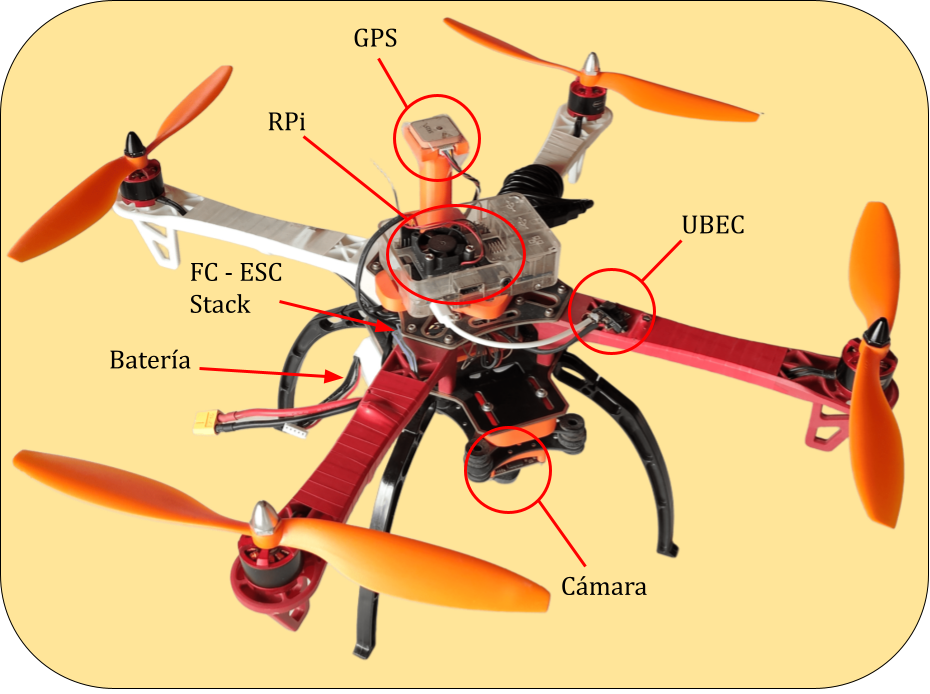
\includegraphics[width=0.75\textwidth]{dron_general_anotado.png}
\caption{Vista general de la plataforma aérea desarrollada, con los componentes principales señalados: GPS, Raspberry Pi, stack FC/ESC, BEC, batería y cámara.}
\label{fig:dron-general}
\end{figure}

\section{Metodología general}
\label{sec:introduccion-metodologia}

La metodología seguida en el proyecto se estructura en fases. En primer lugar se seleccionan los componentes y se monta la plataforma aérea. A continuación se configura el controlador de vuelo mediante herramientas de estación de tierra, se calibra la electrónica principal y se comprueba la estabilidad del sistema. Después se integra la Raspberry Pi con la cámara y con el flujo de telemetría MAVLink, de forma que cada sesión de vuelo genere un conjunto de imágenes y un archivo CSV con la información temporal y de navegación.

Una vez obtenidos los datos de vuelo, se descarga un mosaico satelital de la zona, se divide en parches georreferenciados y se construye una galería visual. Cada imagen capturada por el dron se compara con esta galería mediante una fase de recuperación global y una fase posterior de emparejamiento local. Finalmente se calcula la posición estimada y se compara con la telemetría GNSS registrada durante el vuelo, que se utiliza como referencia para cuantificar el error.

\section{Estructura de la memoria}
\label{sec:introduccion-estructura}

La memoria se organiza de la siguiente forma. El \autoref{cap:objetivos-competencias} (\nameref{cap:objetivos-competencias}) recoge los objetivos y competencias asociadas. El \autoref{cap:estado-arte} (\nameref{cap:estado-arte}) resume los conceptos necesarios sobre navegación de drones, MAVLink y geolocalización visual. El \autoref{cap:diseno-sistema} (\nameref{cap:diseno-sistema}) describe la arquitectura general del sistema. Los capítulos \ref{cap:integracion-hardware} (\nameref{cap:integracion-hardware}) y \ref{cap:integracion-software} (\nameref{cap:integracion-software}) detallan la integración física y lógica de la plataforma. El \autoref{cap:geolocalizacion-visual} (\nameref{cap:geolocalizacion-visual}) presenta el flujo de CVGL utilizado. El \autoref{cap:experimentos-resultados} (\nameref{cap:experimentos-resultados}) documenta los vuelos, métricas y resultados obtenidos. El \autoref{cap:planificacion-presupuesto} (\nameref{cap:planificacion-presupuesto}) incluye la planificación y el presupuesto, y por último el \autoref{cap:conclusiones} (\nameref{cap:conclusiones}) recoge las conclusiones y líneas futuras.

% ---------------------------------------------------------------------

% ---------------------------------------------------------------------
% Objetivos y competencias
% ---------------------------------------------------------------------

\chapter{Objetivos y competencias}
\label{cap:objetivos-competencias}

\begin{Resumen}
En este capítulo se definen el objetivo general, los objetivos específicos y la relación del trabajo con las competencias de la titulación. También se delimitan las restricciones técnicas que condicionan el desarrollo del sistema.
\end{Resumen}

\section{Objetivo general}
\label{sec:objetivo-general}

El objetivo general del Trabajo de Fin de Grado es diseñar, ensamblar e integrar un dron personalizado que sirva como banco de pruebas para navegación autónoma basada en visión, permitiendo capturar imágenes y telemetría en vuelo real y evaluar posteriormente un algoritmo de Geolocalización Visual Cruzada.

\section{Objetivos específicos}
\label{sec:objetivos-especificos}

Para alcanzar el objetivo general se plantean los siguientes objetivos específicos:

\begin{enumerate}
\item Seleccionar e integrar los componentes mecánicos, eléctricos y electrónicos necesarios para construir una plataforma aérea funcional.
\item Configurar el controlador de vuelo, el módulo GPS con brújula y los parámetros básicos de seguridad y estabilidad.
\item Integrar una Raspberry Pi con una cámara USB de obturador global para capturar imágenes durante el vuelo.
\item Establecer un enlace de telemetría basado en MAVLink que permita registrar actitud, rumbo, altitud y posición durante la misión.
\item Preparar un flujo de trabajo para ejecutar misiones mediante estación de tierra y mantener acceso remoto mediante Tailscale y sesiones persistentes con \texttt{tmux}.
\item Construir una base de datos georreferenciada a partir de imágenes satelitales de la zona de vuelo.
\item Evaluar un pipeline de CVGL basado en recuperación global y emparejamiento local sobre las imágenes reales capturadas.
\item Analizar las limitaciones de ejecutar el procesamiento visual a bordo y proponer mejoras futuras para acercar el sistema al tiempo real.
\end{enumerate}

\section{Restricciones de diseño}
\label{sec:restricciones-diseno}

El diseño del sistema está condicionado por las restricciones propias de una plataforma aérea ligera. Las más relevantes son:

\begin{itemize}
\item \textbf{Peso}: todos los elementos embarcados reducen la autonomía y afectan a la estabilidad del dron.
\item \textbf{Energía}: la batería principal debe alimentar el sistema de propulsión y, mediante reguladores adecuados, la electrónica auxiliar.
\item \textbf{Cómputo}: la Raspberry Pi permite captura y comunicaciones, pero tiene capacidad limitada para ejecutar modelos de visión pesados.
\item \textbf{Vibraciones}: la cámara y la electrónica deben montarse minimizando vibraciones para no degradar la calidad de imagen.
\item \textbf{Comunicaciones}: el enlace remoto debe ser robusto frente a desconexiones puntuales durante la misión.
\item \textbf{Seguridad}: las pruebas deben realizarse de forma incremental, validando primero el sistema en tierra y después en vuelos controlados.
\end{itemize}

\section{Competencias relacionadas}
\label{sec:competencias-relacionadas}

El trabajo se relaciona directamente con varias competencias de la titulación. La \autoref{tab:competencias} resume la contribución prevista de cada una.

\begin{table}[htbp]
\centering
\caption{Relación entre competencias y actividades del proyecto.}
\label{tab:competencias}
\begin{tabularx}{\textwidth}{>{\bfseries}p{0.15\textwidth}X}
\toprule
Competencia & Aplicación en el TFG \\
\midrule
CE10 & Integración de una computadora de borde, cámara, telemetría y controlador de vuelo en un sistema empotrado embarcado. \\
CE14 & Uso de imágenes capturadas por una cámara para estimar localización y evaluar correspondencias visuales con mapas de referencia. \\
CE26 & Aplicación de descriptores visuales y técnicas de aprendizaje automático para reconocimiento visual de lugares. \\
CE34 & Estudio de técnicas de estimación de localización y soporte a la navegación de un robot móvil aéreo. \\
CE42 & Uso de herramientas y sistemas específicos de robótica, estaciones de tierra y protocolos de comunicación para integrar dispositivos externos. \\
\bottomrule
\end{tabularx}
\end{table}

\section{Criterios de éxito}
\label{sec:criterios-exito}

Se considerará que la integración básica del sistema es satisfactoria si el dron puede realizar vuelos controlados, capturar imágenes con marcas temporales, registrar telemetría asociada y generar un conjunto de datos utilizable por el pipeline de CVGL. En una segunda fase, el sistema se evaluará mediante métricas de error de localización, número de correspondencias geométricamente válidas y tiempo de procesamiento por imagen.

% ---------------------------------------------------------------------

% ---------------------------------------------------------------------
% Estado del arte
% ---------------------------------------------------------------------

\chapter{Estado del arte}
\label{cap:estado-arte}

\begin{Resumen}
Este capítulo introduce los conceptos técnicos que sustentan el proyecto: navegación de drones, protocolos de comunicación, computación de borde y geolocalización visual cruzada. El objetivo no es realizar una revisión exhaustiva, sino fijar el marco necesario para justificar las decisiones de diseño adoptadas.
\end{Resumen}

\section{Navegación en drones multirrotor}
\label{sec:estado-navegacion-drones}

Un dron multirrotor mantiene el vuelo mediante el control coordinado de varios motores eléctricos. En un cuadricóptero, la variación de empuje de cada motor permite controlar alabeo, cabeceo, guiñada y empuje vertical. El controlador de vuelo fusiona información de sensores inerciales, barómetro, brújula y GNSS para estabilizar la aeronave y ejecutar modos de vuelo asistidos o autónomos.

Las plataformas basadas en ArduPilot permiten configurar parámetros de vuelo, calibrar sensores, cargar misiones y comunicar telemetría mediante MAVLink \parencite{ardupilot_docs,mavlink_docs}. Esta arquitectura resulta adecuada para un TFG de integración porque separa el control de bajo nivel, ejecutado por el controlador de vuelo, del procesamiento de alto nivel, que puede ejecutarse en una computadora externa.

\section{Limitaciones de la navegación GNSS}
\label{sec:estado-limitaciones-gnss}

El GNSS proporciona una estimación global de posición, pero puede degradarse por multitrayecto, pérdida de visibilidad de satélites, interferencias o ataques de suplantación. En un contexto de navegación autónoma, estas limitaciones justifican el estudio de fuentes de localización complementarias. La visión artificial es especialmente atractiva porque muchas plataformas ya incorporan cámaras para inspección, grabación o percepción del entorno.

\section{Computación de borde en plataformas aéreas}
\label{sec:estado-edge}

La computación de borde consiste en procesar datos cerca del sensor que los genera. En un dron, esto reduce la dependencia de un enlace permanente con tierra y permite tomar decisiones con menor latencia. No obstante, la capacidad de cálculo embarcada está limitada por peso, consumo y disipación térmica. En este proyecto se emplea una Raspberry Pi para captura, almacenamiento y comunicaciones, pero el procesamiento visual completo se evalúa inicialmente fuera de bordo.

\section{Geolocalización Visual Cruzada}
\label{sec:estado-cvgl}

La Geolocalización Visual Cruzada compara una imagen tomada desde una vista determinada con una base de datos georreferenciada capturada desde otra vista. En el caso de un dron, la imagen de consulta procede de la cámara embarcada y la base de datos puede generarse a partir de mapas satelitales o aéreos. El problema es complejo porque existen cambios de escala, orientación, iluminación, estación del año, perspectiva y resolución.

Un enfoque habitual divide el problema en dos etapas. Primero se realiza una recuperación global, en la que cada imagen se representa mediante un descriptor compacto y se buscan candidatos visualmente similares. Después se aplica una verificación local, que calcula correspondencias entre la imagen de consulta y los candidatos seleccionados para estimar una transformación geométrica consistente.

\section{Descriptores globales y emparejamiento local}
\label{sec:estado-descriptores-matching}

Los modelos visuales auto-supervisados como DINOv2 han demostrado capacidad para producir características robustas y transferibles a tareas para las que no fueron entrenados explícitamente \parencite{oquab2023dinov2}. AnyLoc explota precisamente esta propiedad para el reconocimiento visual de lugares (\textit{Visual Place Recognition}, VPR): en vez de entrenar una red específica para cada dominio (interior, urbano, carretera, aéreo\ldots), propone extraer los tokens de parche de un backbone auto-supervisado ya entrenado como DINOv2 --sin ajustarlo a ningún dominio concreto-- y agregarlos en un único descriptor global mediante VLAD, mostrando que este enfoque \textit{zero-shot} generaliza razonablemente bien entre entornos muy distintos entre sí \parencite{keetha2023anyloc}. Este proyecto adopta la misma filosofía --backbone auto-supervisado congelado más agregación, sin entrenar nada específico para el par dron-satélite-- pero comparando explícitamente sus variantes (backbone y agregación) sobre la escena propia, en vez de asumir directamente la configuración del trabajo original (\autoref{sec:estado-alternativas-no-adoptadas}).

DINOv3 es la evolución del backbone anterior, entrenada sobre un conjunto de datos mayor y disponible en variantes especializadas por dominio \parencite{simeoni2025dinov3}. En particular, Meta AI publica una variante entrenada específicamente sobre imágenes de satélite (SAT-493M), que resulta especialmente adecuada para este proyecto porque la galería de referencia es, precisamente, satelital: aunque el dominio \enquote{vista de dron} no esté cubierto por el preentrenamiento, comparte mucha más estructura visual con imágenes de satélite que un backbone entrenado sobre fotografía web genérica.

Como alternativa a la agregación GeM, VLAD (\textit{Vector of Locally Aggregated Descriptors}) construye un vocabulario visual mediante \textit{k-means} sobre los propios parches de la galería y agrega los tokens de cada imagen como residuos respecto a ese vocabulario \parencite{arandjelovic2016netvlad}. El repositorio de referencia de AnyLoc trata VLAD, no GeM, como su variante principal, por lo que en este trabajo se ha comparado empíricamente ambas agregaciones sobre los dos backbones (DINOv2 y DINOv3) en vez de asumir directamente cuál rendiría mejor sobre esta escena concreta (ver \autoref{sec:resultados-recuperacion-global}).

Para la verificación local, LoFTR propone un emparejamiento sin detectores clásicos de puntos clave, basado en transformadores, que puede ser útil cuando las imágenes presentan baja textura o cambios importantes de punto de vista \parencite{sun2021loftr}. Sobre las correspondencias que produce LoFTR, la estimación robusta de la transformación geométrica (homografía) se realiza con MAGSAC++, una variante de RANSAC que no requiere fijar a mano un umbral de error fijo para clasificar inliers/outliers, sino que marginaliza sobre un rango de umbrales, lo que la hace más robusta cuando la proporción de correspondencias erróneas varía mucho de una imagen a otra \parencite{barath2020magsac++}. En este trabajo se emplea esta combinación (LoFTR + MAGSAC++) para validar geométricamente los candidatos obtenidos en la fase global y estimar una posición final sobre el mosaico satelital.

\subsection{Alternativas evaluadas y no adoptadas}
\label{sec:estado-alternativas-no-adoptadas}

Varias decisiones de diseño del pipeline final (\autoref{cap:geolocalizacion-visual}) se tomaron tras comparar empíricamente varias alternativas, no por adopción directa de lo propuesto en la literatura:

\begin{itemize}
\item \textbf{GeM+DINOv2 frente a VLAD+DINOv3-SAT}: la configuración originalmente prevista (GeM sobre DINOv2, siguiendo el enfoque más simple de AnyLoc) obtenía una precisión de recuperación global muy baja sobre la escena real de vuelo. Cambiar a VLAD+DINOv3-SAT mejoró sustancialmente el \textit{ranking} del parche correcto (ver \autoref{sec:resultados-recuperacion-global}).
\item \textbf{Calibración de la cámara}: se calibró la cámara (parámetros intrínsecos y distorsión, método de Zhang) y se probó a corregir la distorsión de las imágenes antes de la recuperación y el emparejamiento. El resultado fue una ligera pérdida de precisión, no una mejora, atribuible a un artefacto de deformación en los bordes introducido por \texttt{cv2.undistort} con un campo de visión tan amplio ($\approx$\ang{120}). Se descartó esta corrección en la versión final (ver \autoref{sec:problemas-hardware}).
\item \textbf{\textit{Batching} de LoFTR}: procesar varios pares candidato-consulta en el mismo lote de LoFTR ofrecía una mejora de tiempo modesta a cambio de un mayor riesgo de agotar memoria de GPU; se descartó en favor de la estrategia de \textit{early-exit} (parar en cuanto un candidato supera un umbral de \textit{inliers}).
\item \textbf{EfficientLoFTR}: una variante más ligera de LoFTR no superó en la práctica al LoFTR ya optimizado con \textit{early-exit}, precisión FP16 y tamaño de imagen reducido.
\end{itemize}

\section{Herramientas de estación de tierra}
\label{sec:estado-estaciones-tierra}

Las estaciones de tierra facilitan la configuración y operación de la aeronave. En este proyecto se utiliza Mission Planner para configurar y calibrar el dron, mientras que QGroundControl se emplea para cargar misiones de forma más cómoda durante las pruebas \parencite{qgroundcontrol_docs}. Esta combinación permite separar la fase de parametrización del controlador de vuelo de la planificación operativa de misiones.

% ---------------------------------------------------------------------

% ---------------------------------------------------------------------
% Diseño general del sistema
% ---------------------------------------------------------------------

\chapter{Diseño general del sistema}
\label{cap:diseno-sistema}

\begin{Resumen}
Este capítulo describe la arquitectura global del sistema desarrollado. Se identifican los bloques funcionales, los componentes seleccionados y los flujos de energía, datos y control que permiten convertir el dron en un banco de pruebas para navegación visual.
\end{Resumen}

\section{Arquitectura funcional}
\label{sec:arquitectura-funcional}

El sistema se divide en seis bloques funcionales, cada uno con una responsabilidad delimitada:

\begin{description}
\item[Plataforma mecánica.] Estructura física del dron: chasis, brazos y tren de aterrizaje, junto con las piezas impresas en 3D diseñadas a medida para fijar el resto de componentes sobre ella (\autoref{sec:modelos-3d}).
\item[Propulsión.] Motores brushless y hélices; generan el empuje necesario para el vuelo.
\item[Alimentación.] Distribuye la energía de la batería principal en dos líneas separadas: una directa hacia el ESC y los motores, y otra regulada mediante un BEC hacia la electrónica auxiliar (\autoref{sec:flujo-energia}).
\item[Control de vuelo.] El controlador de vuelo (FC) estabiliza la aeronave, ejecuta la misión y centraliza la lectura de los sensores de navegación (GPS, brújula, IMU).
\item[Percepción.] Cámara USB conectada a la Raspberry Pi; captura las imágenes que usa el pipeline de geolocalización visual (\autoref{cap:geolocalizacion-visual}).
\item[Comunicaciones.] Dongle LTE combinado con Tailscale (\autoref{sec:que-es-tailscale}); permite monitorizar el sistema y acceder de forma remota a la Raspberry Pi durante las pruebas de vuelo.
\end{description}

Estos bloques se relacionan entre sí mediante dos flujos independientes, detallados en las siguientes secciones: el flujo de energía (\autoref{sec:flujo-energia}), que reparte la potencia de la batería entre propulsión y electrónica auxiliar, y el flujo de datos (\autoref{sec:flujo-datos}), que lleva la telemetría del controlador de vuelo y las imágenes de la cámara desde la Raspberry Pi hasta el ordenador de procesado.

\section{Componentes principales}
\label{sec:componentes-principales}

La \autoref{tab:componentes} resume los componentes utilizados en la plataforma. Los nombres se mantienen cercanos a la denominación comercial para facilitar su trazabilidad durante la redacción final.

\begin{longtable}{p{0.28\textwidth}p{0.30\textwidth}p{0.34\textwidth}}
\caption{Componentes principales del sistema.}\label{tab:componentes}\\
\toprule
\textbf{Bloque} & \textbf{Componente} & \textbf{Función} \\
\midrule
\endfirsthead
\toprule
\textbf{Bloque} & \textbf{Componente} & \textbf{Función} \\
\midrule
\endhead
Estructura & Chasis F450 negro con tren de aterrizaje & Soporte mecánico de la plataforma cuadricóptero. \\
Propulsión & Motores brushless Readytosky 2212 920KV & Generación de empuje en cada brazo del dron. \\
Propulsión & Hélices 1045 de 10x4,5 pulgadas CW/CCW & Conversión del par de los motores en empuje vertical. \\
Alimentación & Batería LiPo 4S 5200 mAh 60C con conector XT60 & Fuente principal de energía del sistema. \\
Alimentación & BEC QITN ajustable 6--60 V a 5/9/12 V & Regulación de tensión para electrónica auxiliar. \\
Control & Stack H743 6S con ESC de 55 A & Controlador de vuelo y etapa de potencia para motores. \\
Navegación & Módulo GPS M10 10 Hz con brújula & Posicionamiento GNSS y referencia de rumbo. \\
Seguridad & Receptor de radiocontrol FlySky FS-i6X & Permite tomar el control manual del dron durante la misión ante un comportamiento anómalo o para cancelar el vuelo. \\
Percepción & Cámara USB Svpro 2 MP global shutter AR0234 & Captura de imágenes para geolocalización visual. \\
Procesamiento & Raspberry Pi & Captura, almacenamiento de datos, telemetría y acceso remoto. \\
Comunicaciones & Dongle LTE y Tailscale & Enlace remoto para monitorización y acceso al sistema. \\
Aislamiento & Placa antivibración de fibra de carbono & Reducción de vibraciones en cámara o elementos sensibles. \\
\bottomrule
\end{longtable}

\section{Flujo de energía}
\label{sec:flujo-energia}

La batería LiPo 4S alimenta el sistema principal de potencia. Desde esta fuente se suministra energía al ESC integrado en el stack para accionar los motores. La electrónica auxiliar requiere tensiones reguladas, por lo que se utiliza un BEC ajustable para alimentar los dispositivos que no pueden conectarse directamente a la batería principal. Esta separación evita someter la Raspberry Pi, la cámara y otros periféricos a tensiones o ruidos eléctricos no adecuados.

\section{Flujo de datos}
\label{sec:flujo-datos}

El controlador de vuelo genera telemetría MAVLink con información de actitud, altitud, posición y rumbo. Esta telemetría se reenvía mediante MAVProxy hacia el ordenador de tierra y hacia la Raspberry Pi. La cámara USB envía imágenes a la Raspberry Pi, donde se almacenan junto con un archivo CSV de telemetría sincronizada. Posteriormente, los datos se transfieren al ordenador de procesado para ejecutar el pipeline de CVGL.

\section{Decisiones de diseño}
\label{sec:decisiones-diseno}

Se ha optado por una arquitectura modular para facilitar la depuración. El controlador de vuelo mantiene la responsabilidad de estabilización y seguridad, mientras que la Raspberry Pi se encarga de tareas no críticas como captura, registro y comunicaciones. Esta separación reduce el riesgo de que una sobrecarga de procesamiento visual afecte al control de vuelo.

La ejecución de la geolocalización visual se deja inicialmente fuera de bordo. Esta decisión responde a la carga computacional de los modelos de visión empleados y permite validar el flujo completo con imágenes reales antes de optimizarlo. Una futura versión podría sustituir la Raspberry Pi por una computadora con aceleración GPU o adaptar los modelos para inferencia ligera.

% ---------------------------------------------------------------------

% ---------------------------------------------------------------------
% Integración hardware
% ---------------------------------------------------------------------

\chapter{Integración hardware}
\label{cap:integracion-hardware}

\begin{Resumen}
Este capítulo documenta el montaje físico y eléctrico de la plataforma. Se describen la estructura, el sistema de propulsión, la alimentación, el controlador de vuelo, el módulo de navegación, la cámara y la computadora de borde.
\end{Resumen}

\section{Montaje de la estructura}
\label{sec:montaje-estructura}

La plataforma se basa en un chasis tipo F450, adecuado para un cuadricóptero de tamaño medio. Este formato ofrece suficiente espacio para distribuir la batería, el controlador de vuelo, el GPS, la Raspberry Pi y el sistema de cámara, manteniendo una estructura relativamente sencilla de montar y reparar.

Durante el montaje se debe prestar especial atención a la orientación de los brazos, el sentido de giro de cada motor, la fijación de las hélices y la ubicación del centro de gravedad (Figuras \ref{fig:vista-planta-helices} y \ref{fig:vista-lateral}). Una distribución equilibrada reduce el esfuerzo de control y mejora la estabilidad durante el vuelo.

\begin{figure}[htbp]
\centering
\begin{minipage}[b]{0.48\textwidth}
\centering
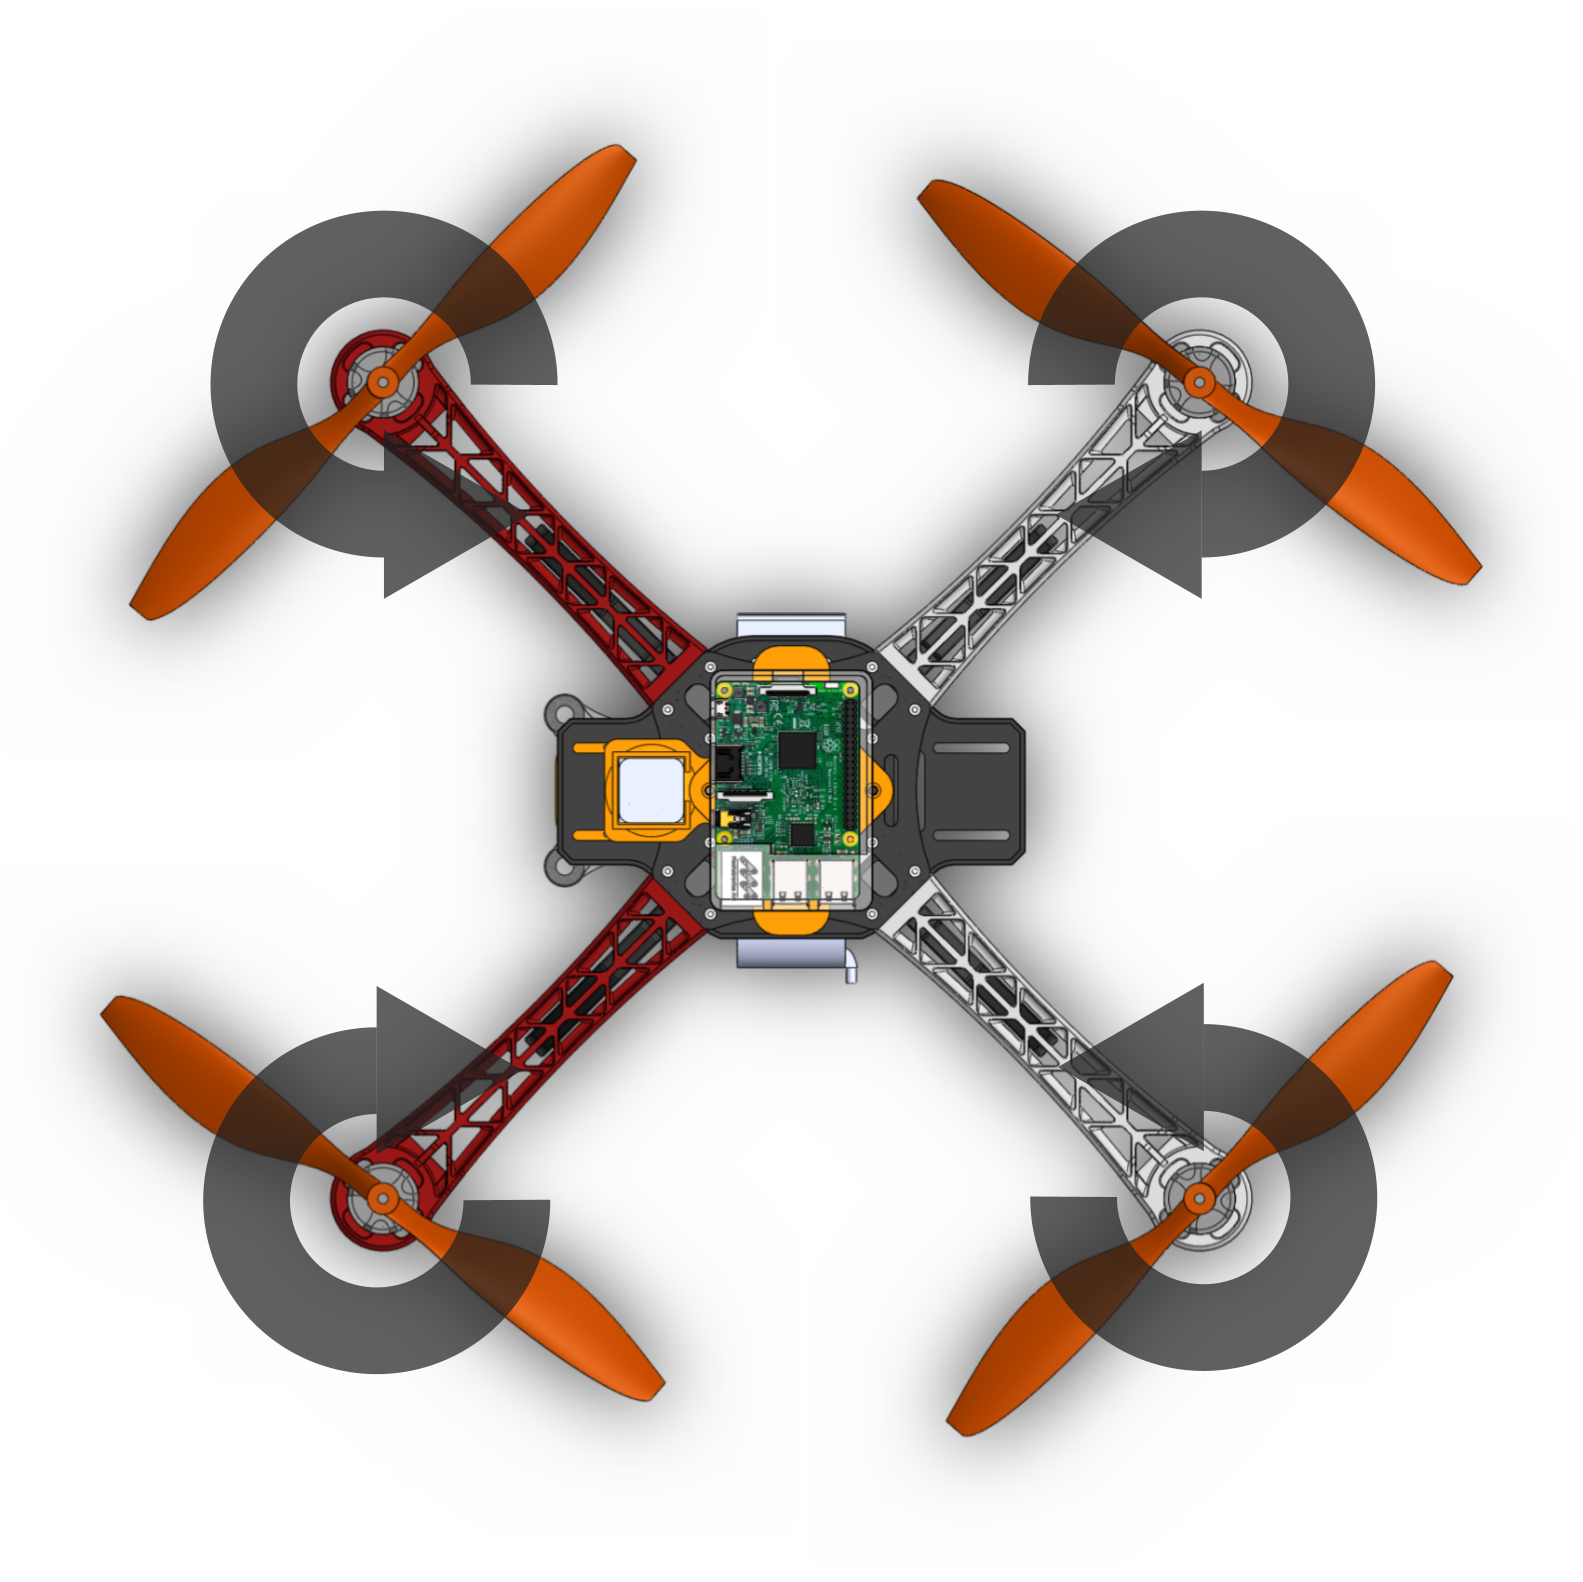
\includegraphics[width=\textwidth]{vista_planta_helices.png}
\caption{Vista en planta: sentido de giro de cada motor (brazos rojos y brazos grises giran en sentidos opuestos, configuración en X).}
\label{fig:vista-planta-helices}
\end{minipage}
\hfill
\begin{minipage}[b]{0.48\textwidth}
\centering
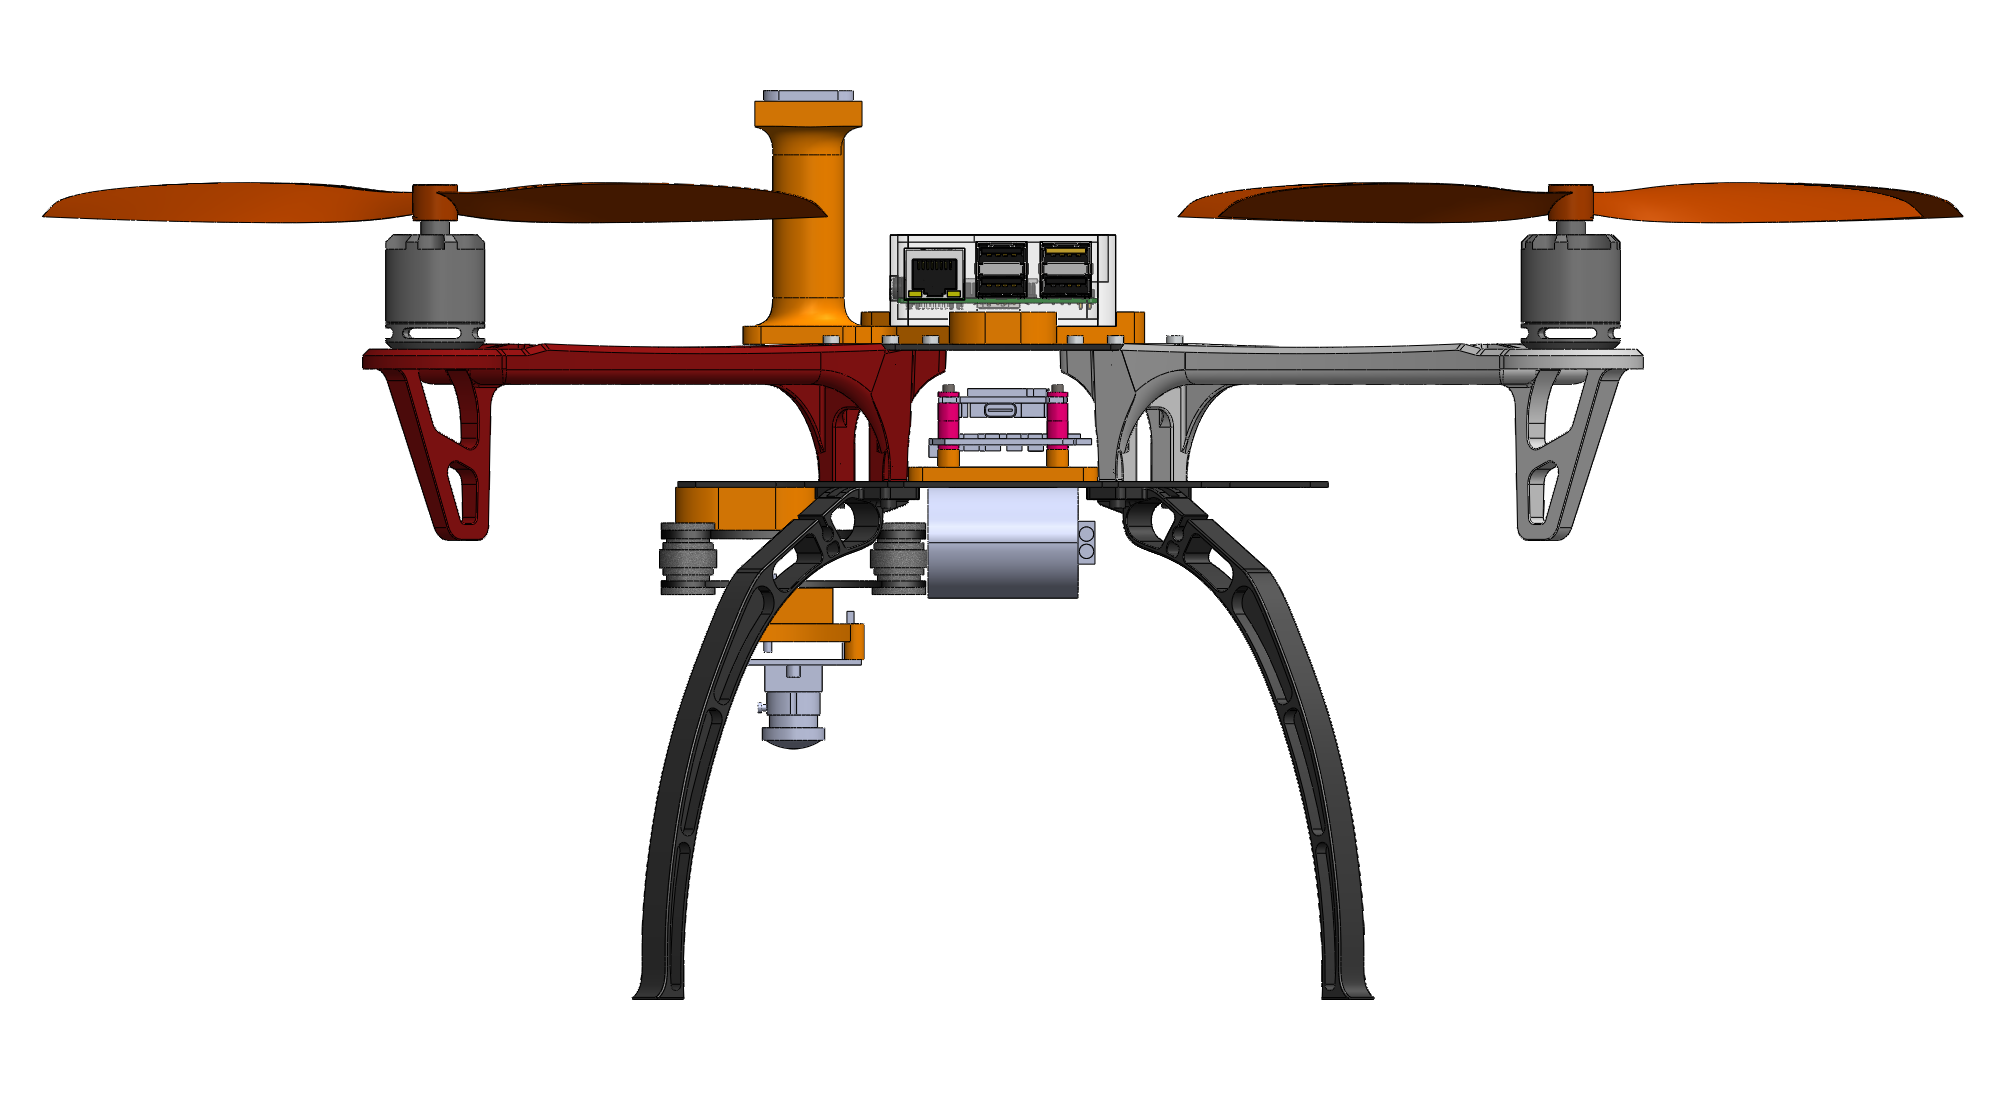
\includegraphics[width=\textwidth]{vista_lateral.png}
\caption{Vista lateral: distribución de las piezas sobre el chasis, con la batería montada bajo el mismo.}
\label{fig:vista-lateral}
\end{minipage}
\end{figure}

\subsection{Peso y ubicación de la batería}
\label{sec:peso-bateria}

La batería es, con diferencia, el componente más pesado de toda la plataforma: el dron completo sin batería pesa \SI{980}{\gram}, mientras que la batería por sí sola pesa \SI{390}{\gram} —cerca del 28\,\% del peso total del conjunto ya con batería (\SI{1370}{\gram})—. Por este motivo, su ubicación es una de las decisiones de diseño más importantes para la estabilidad de vuelo: se ha montado bajo el chasis, no sobre él (visible en la \autoref{fig:vista-lateral}), lo que baja el centro de gravedad del conjunto y evita los problemas de estabilidad que aparecerían si se montara en una posición más alta, con la mayor parte del peso concentrado por encima del plano de los motores.

\section{Modelos 3D y piezas impresas}
\label{sec:modelos-3d}

Se partió de un modelo 3D base del dron ya existente, con el chasis F450 y los motores, sobre el cual se modelaron los seis componentes principales que había que integrar (\autoref{fig:modelo3d-componentes}): la batería, la placa antivibración, la Raspberry Pi (con su caja), el stack FC/ESC, la cámara y el módulo GPS. Ninguno de estos componentes estaba pensado de fábrica para fijarse directamente al chasis F450, por lo que fue necesario diseñar e imprimir en 3D piezas adaptadoras específicas para cada uno (\autoref{fig:piezas-impresas-adaptadores}): tres adaptadores para la fijación de la cámara, una torre elevadora para el GPS —que resuelve el problema de proximidad descrito en la \autoref{sec:problema-gps-proximidad}— y un adaptador para fijar el stack FC/ESC al chasis. Estas piezas ya son visibles, montadas, en la fotografía general del dron de la \autoref{fig:dron-general}.

\begin{figure}[htbp]
\centering
\begin{minipage}[b]{0.48\textwidth}
\centering
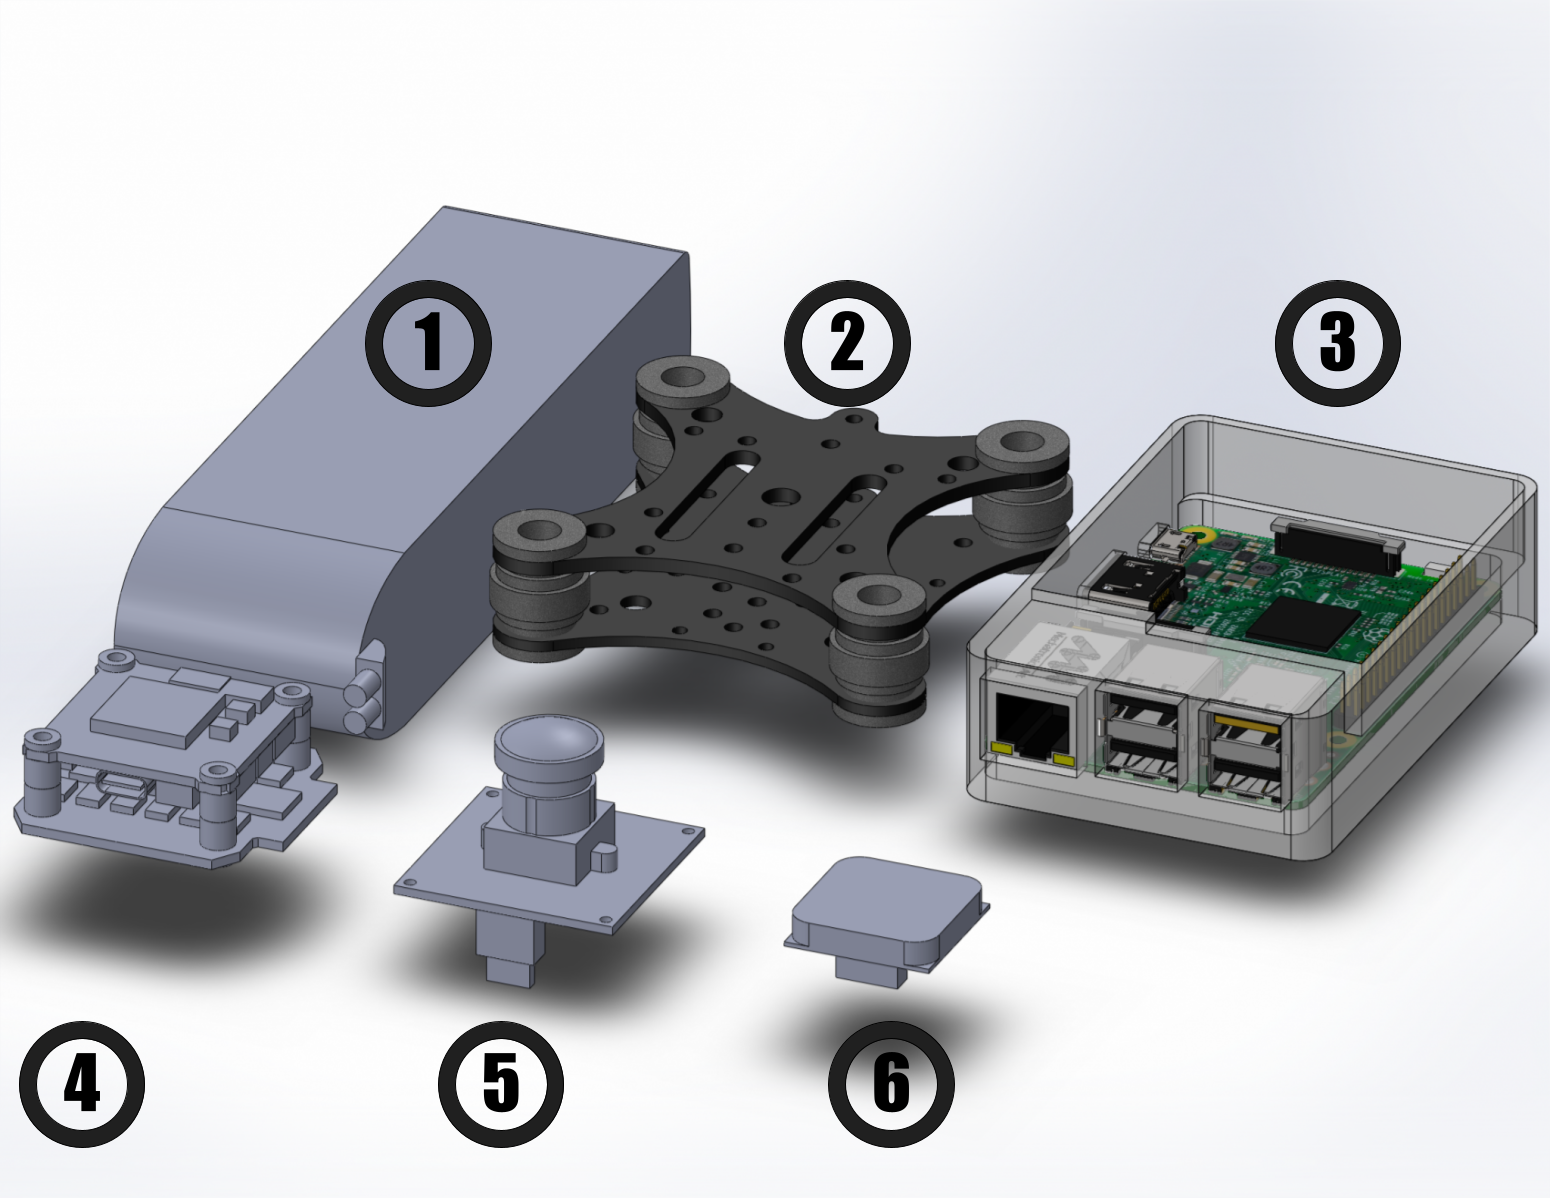
\includegraphics[width=\textwidth]{modelo3d_componentes.png}
\caption{Componentes principales modelados en 3D: 1) batería, 2) placa antivibración, 3) Raspberry Pi (con caja), 4) stack FC/ESC, 5) cámara, 6) módulo GPS.}
\label{fig:modelo3d-componentes}
\end{minipage}
\hfill
\begin{minipage}[b]{0.48\textwidth}
\centering
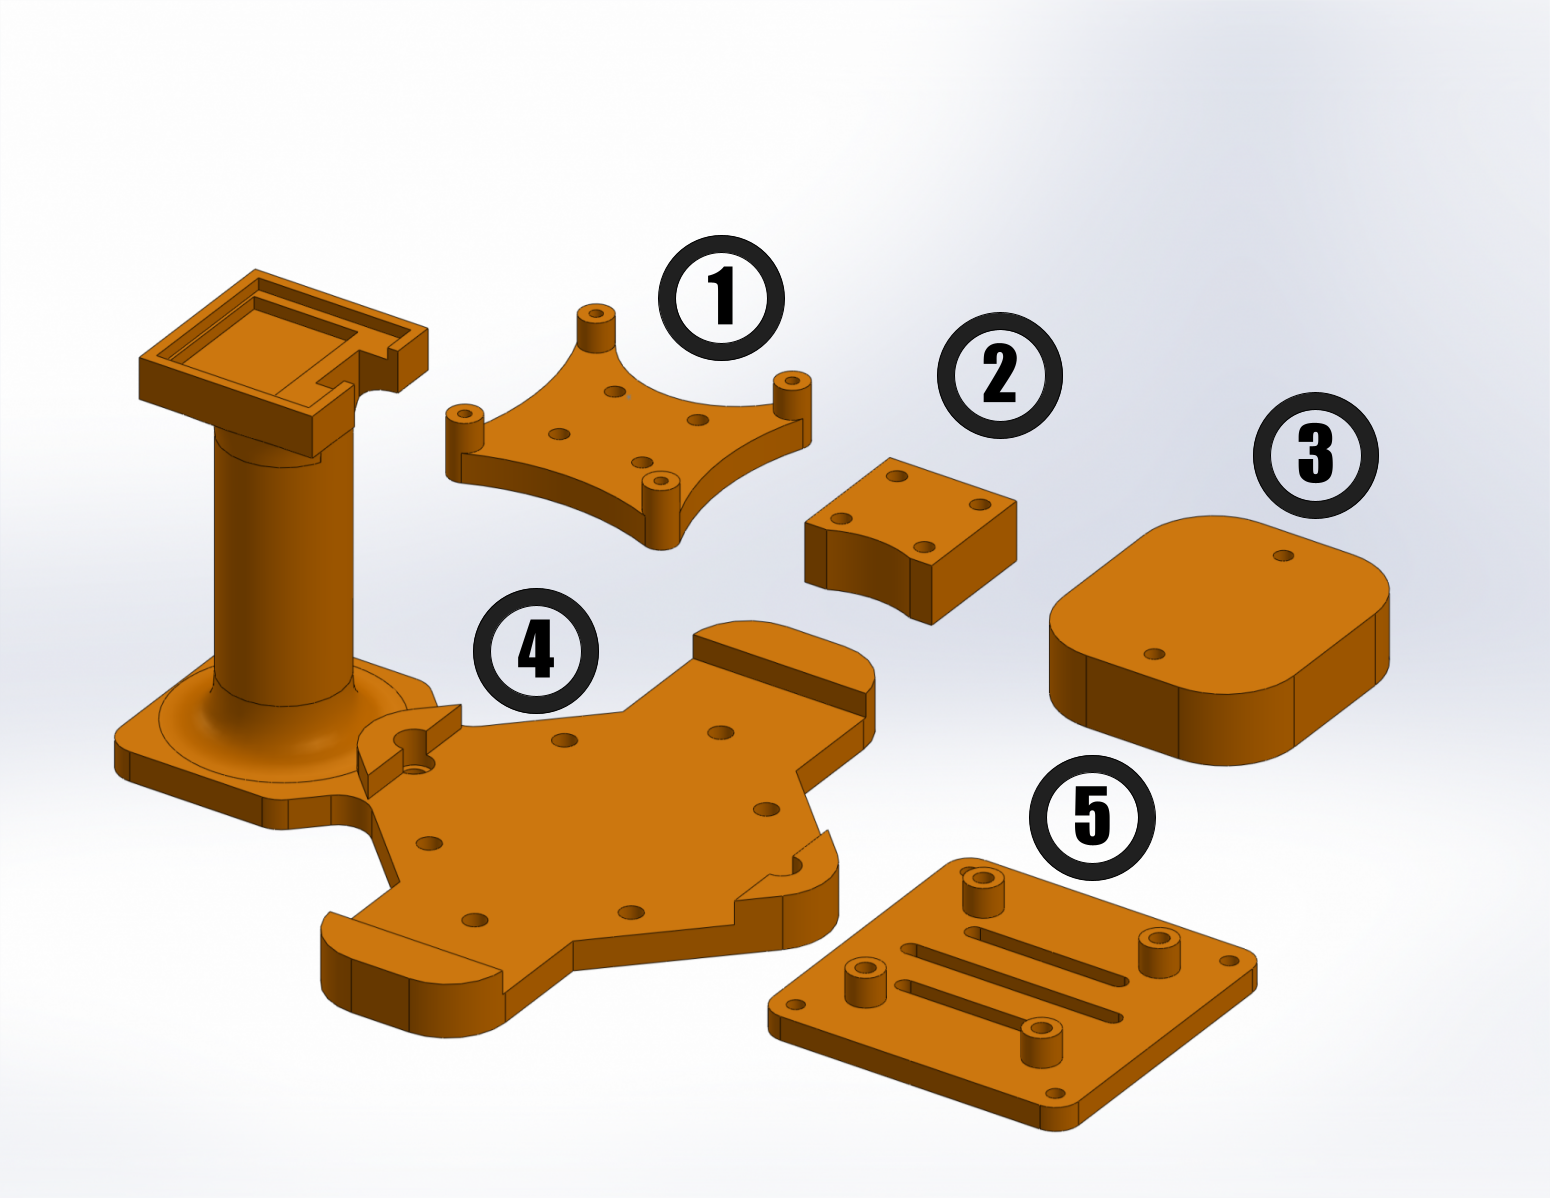
\includegraphics[width=\textwidth]{piezas_impresas_adaptadores.png}
\caption{Piezas diseñadas e impresas en 3D para fijar los componentes al chasis: 1--3) adaptadores de la cámara, 4) torre elevadora del GPS, 5) adaptador del stack FC/ESC al chasis.}
\label{fig:piezas-impresas-adaptadores}
\end{minipage}
\end{figure}

\section{Sistema de propulsión}
\label{sec:sistema-propulsion}

El sistema de propulsión está formado por cuatro motores brushless 2212 de 920KV y hélices 1045 CW/CCW. La combinación de motores, hélices y batería 4S debe proporcionar empuje suficiente para elevar la plataforma con la carga adicional de cámara, Raspberry Pi y comunicaciones.

Antes de instalar las hélices se recomienda comprobar individualmente el sentido de giro de cada motor desde la estación de tierra. Esta prueba reduce el riesgo de vuelco durante el primer armado. Las hélices deben instalarse únicamente después de verificar el orden de motores y realizar las pruebas de seguridad necesarias.

\section{Alimentación eléctrica}
\label{sec:alimentacion-electrica}

La batería principal es una LiPo 4S de \SI{5200}{\milli\ampere\hour} y descarga 60C. La tensión nominal del conjunto es de \SI{14.8}{\volt}. El stack de control y ESC se alimenta desde la batería principal, mientras que la electrónica auxiliar requiere una línea regulada. Para ello se incorpora un BEC ajustable capaz de entregar tensiones de 5, 9 o \SI{12}{\volt} según la configuración seleccionada.

La \autoref{fig:alimentacion-dron} esquematiza esta ruta de alimentación, indicando los conectores, la masa común y la tensión usada por cada dispositivo.

\begin{figure}[htbp]
\centering
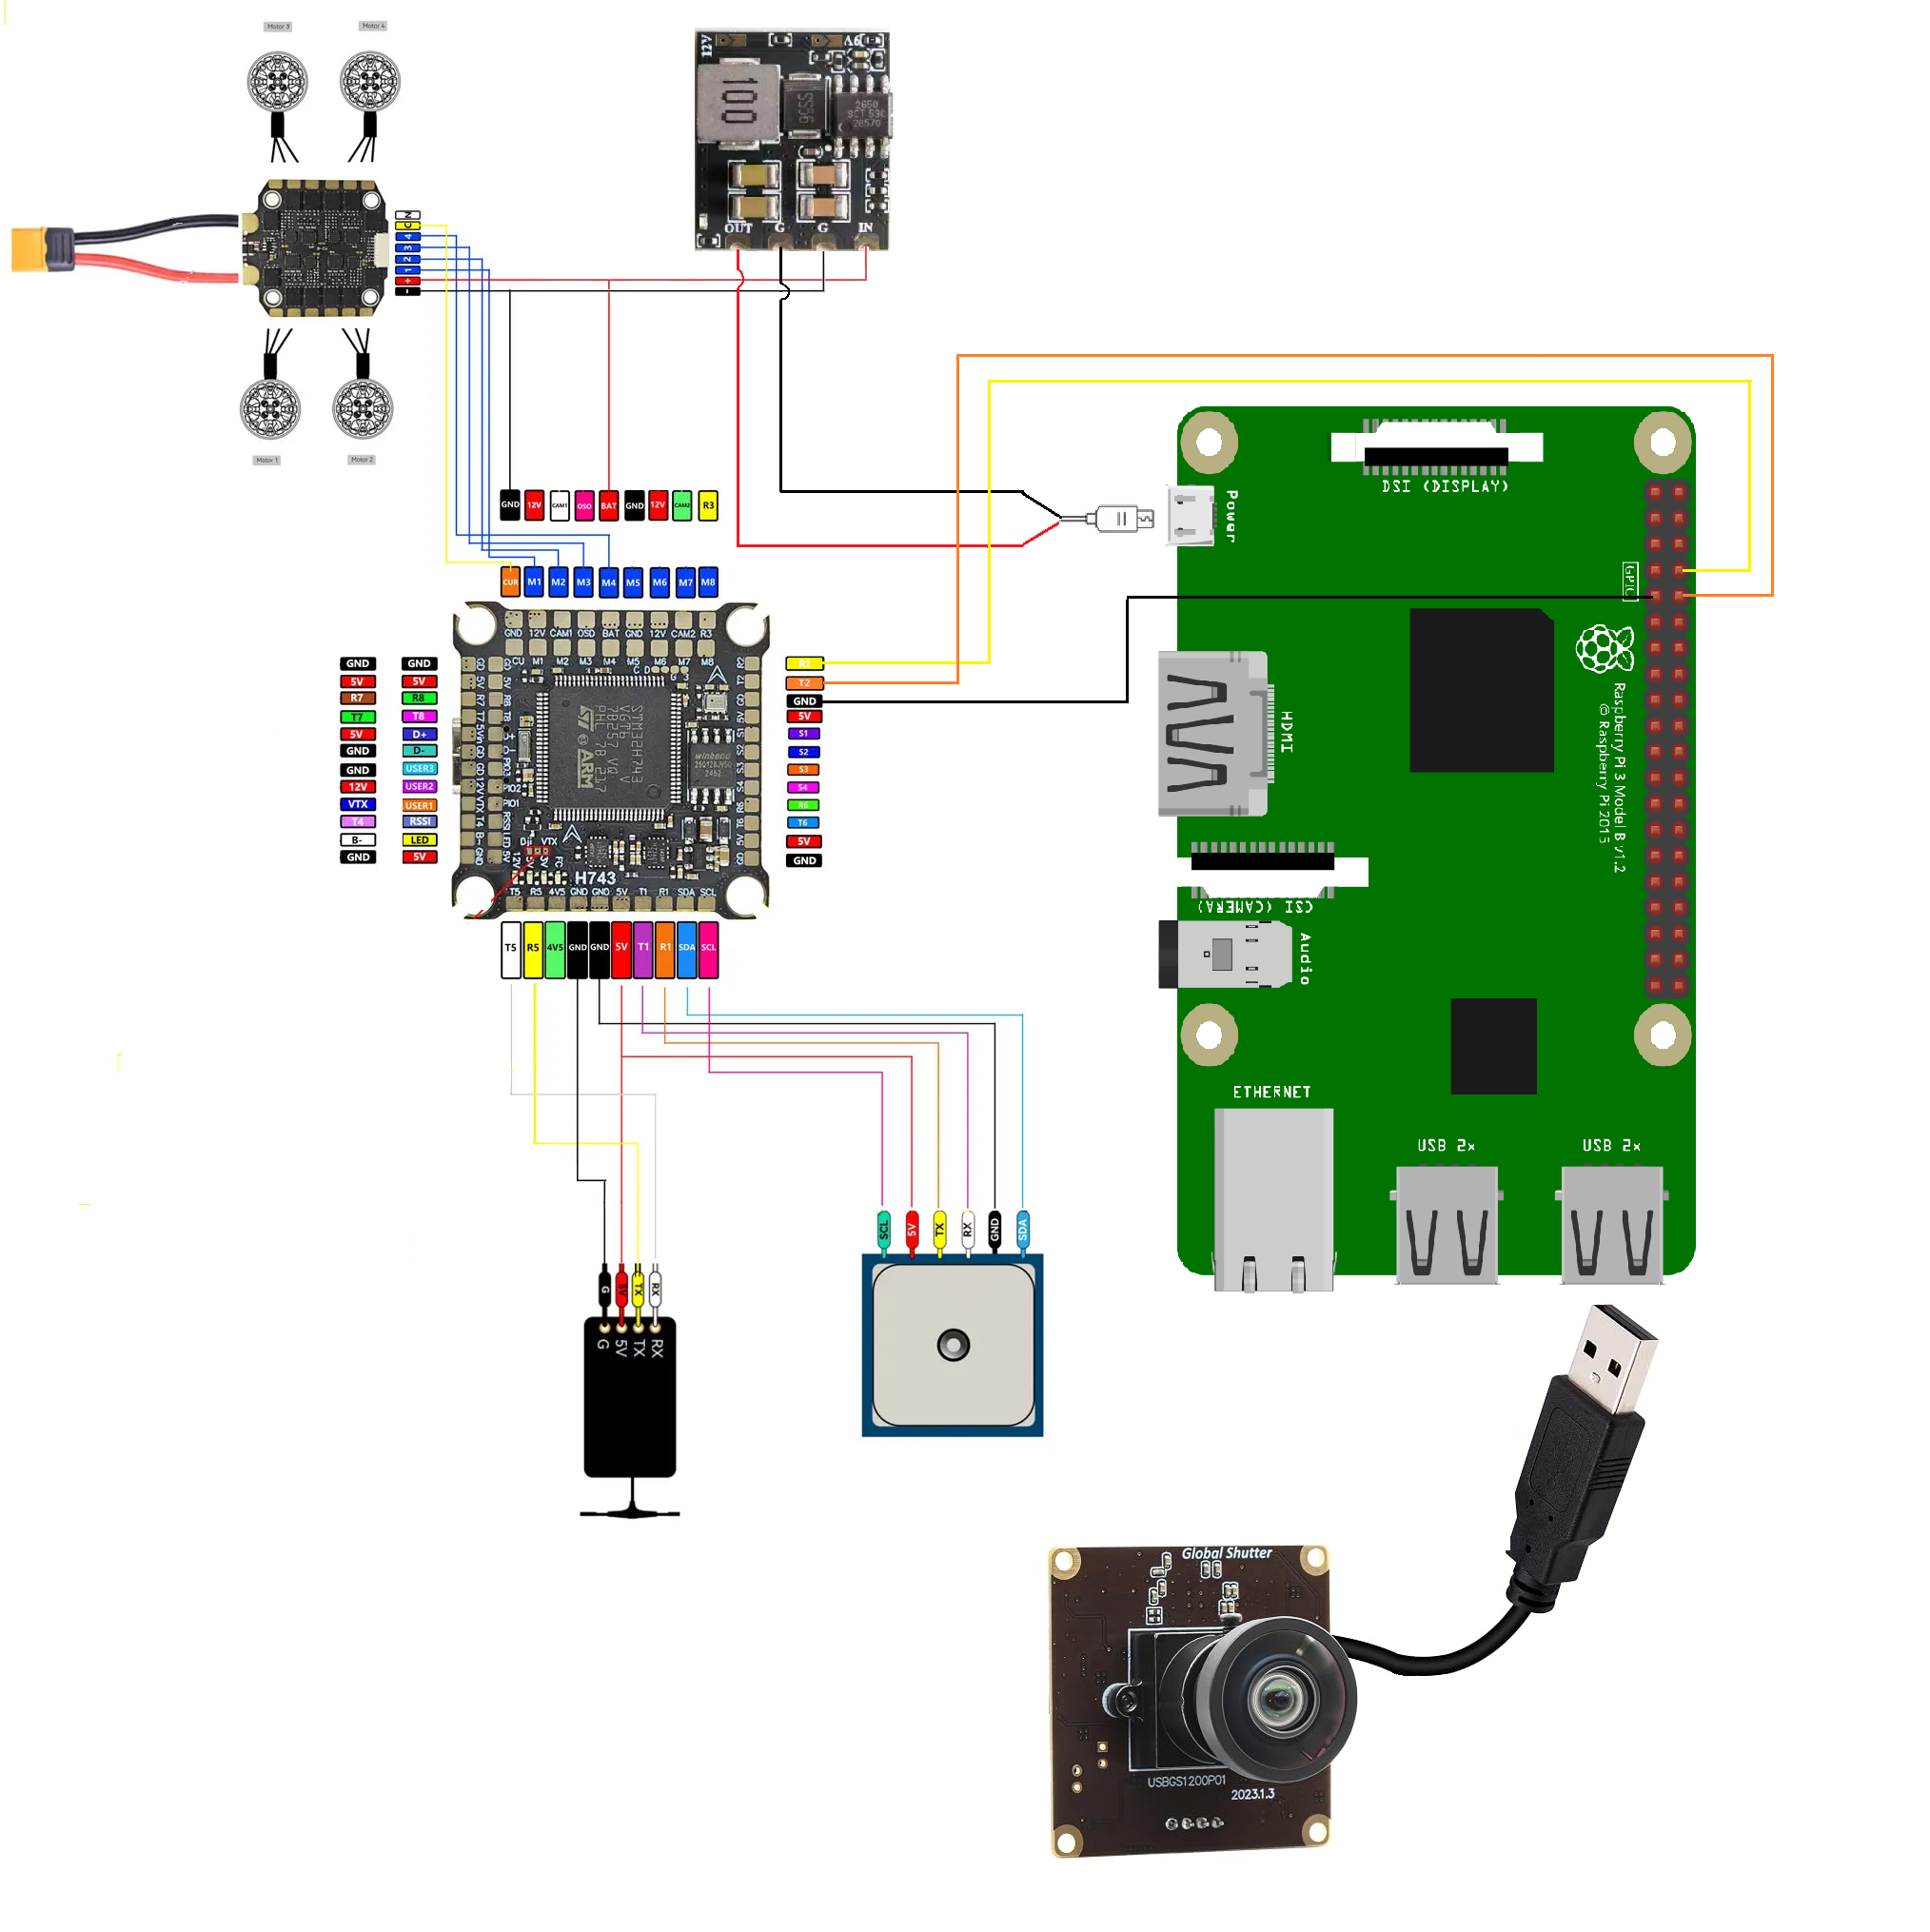
\includegraphics[width=0.85\textwidth]{circuito_electrico.png}
\caption{Distribución de alimentación eléctrica y de datos del dron: batería, ESC/motores, BEC, controlador de vuelo (FC), Raspberry Pi, GPS/brújula y cámara.}
\label{fig:alimentacion-dron}
\end{figure}

\section{Controlador de vuelo y sensores}
\label{sec:controlador-sensores}

El controlador de vuelo utilizado es un stack H743 6S con ESC de 55 A. Este elemento centraliza la lectura de sensores, la estabilización de la aeronave y la generación de señales de control para los motores. El módulo GPS M10 con brújula proporciona posición global y rumbo magnético, información utilizada tanto por el controlador de vuelo como por el registro de datos.

La instalación del GPS debe realizarse alejada de fuentes de interferencia electromagnética, especialmente cables de potencia y reguladores. La orientación física del módulo debe coincidir con la configuración establecida en el firmware para evitar errores de rumbo.

El dron incorpora además un receptor de radiocontrol FlySky FS-i6X, conectado a la FC junto al resto de periféricos (\autoref{sec:conexiones-electricas-datos}). Aunque la misión se ejecuta de forma autónoma mediante los \textit{waypoints} cargados en el controlador de vuelo, el receptor se mantiene activo durante todo el vuelo como mecanismo de seguridad: permite tomar el control manual del dron en cualquier momento con la emisora asociada, tanto para corregir un comportamiento anómalo como para cancelar la misión y aterrizar de forma controlada.

\section{Cámara y montaje antivibración}
\label{sec:camara-montaje}

La cámara seleccionada es una Svpro USB de 2 MP con sensor AR0234, obturador global, resolución de 1920x1200 píxeles y lente gran angular. Para mejorar la calidad de las imágenes se incorpora una placa antivibración de fibra de carbono. La orientación de la cámara debe documentarse con precisión, ya que afecta a la interpretación geométrica de las imágenes y al emparejamiento con el mosaico satelital.

\subsection{Obturador global frente a obturador rodante}
\label{sec:global-vs-rolling-shutter}

La elección de un sensor de \textbf{obturador global} (\textit{global shutter}) frente a uno de \textbf{obturador rodante} (\textit{rolling shutter}) no es indiferente en una plataforma en movimiento. Un sensor de obturador rodante expone cada fila de píxeles en un instante ligeramente distinto, escaneando la imagen de arriba a abajo en vez de capturar el fotograma completo de forma simultánea. Si la cámara (o la escena) se mueve apreciablemente durante ese barrido —como ocurre en un dron, donde a la traslación se suman las vibraciones de los motores y las hélices—, el resultado es una imagen con deformación geométrica dependiente de la fila (\textit{skew}, efecto de \enquote{cizalla}): líneas rectas del mundo real aparecen inclinadas, y el desplazamiento entre la parte superior e inferior de la imagen no corresponde a ninguna transformación geométrica simple.

Esta deformación es especialmente perjudicial para este proyecto porque el pipeline de geolocalización visual (\autoref{cap:geolocalizacion-visual}) depende de estimar una homografía —una transformación geométrica global y consistente— entre la imagen del dron y el parche satelital. Una imagen con \textit{skew} de obturador rodante no es geométricamente consistente con una homografía única, lo que degrada tanto el número de correspondencias válidas que encuentra LoFTR como la precisión de la posición proyectada. Un sensor de obturador global, en cambio, expone todos los píxeles del fotograma en el mismo instante, por lo que la imagen resultante es geométricamente consistente con independencia del movimiento del dron durante la captura.

Se dispone de una cámara de cada tipo (Svpro AR0234, obturador global, la usada en el proyecto; y una cámara adicional de obturador rodante) para poder comparar directamente el efecto sobre las imágenes capturadas en vuelo (\autoref{fig:frame-rolling} y \autoref{fig:frame-global}). Ambos fotogramas se capturaron con la cámara montada sobre la misma placa antivibración de fibra de carbono, de forma que la comparación aísla el efecto del tipo de obturador y no una diferencia en el aislamiento mecánico. En el fotograma de obturador rodante se aprecia una ondulación característica en la imagen, ausente en el de obturador global.

\begin{figure}[htbp]
\centering
\begin{minipage}[b]{0.48\textwidth}
\centering
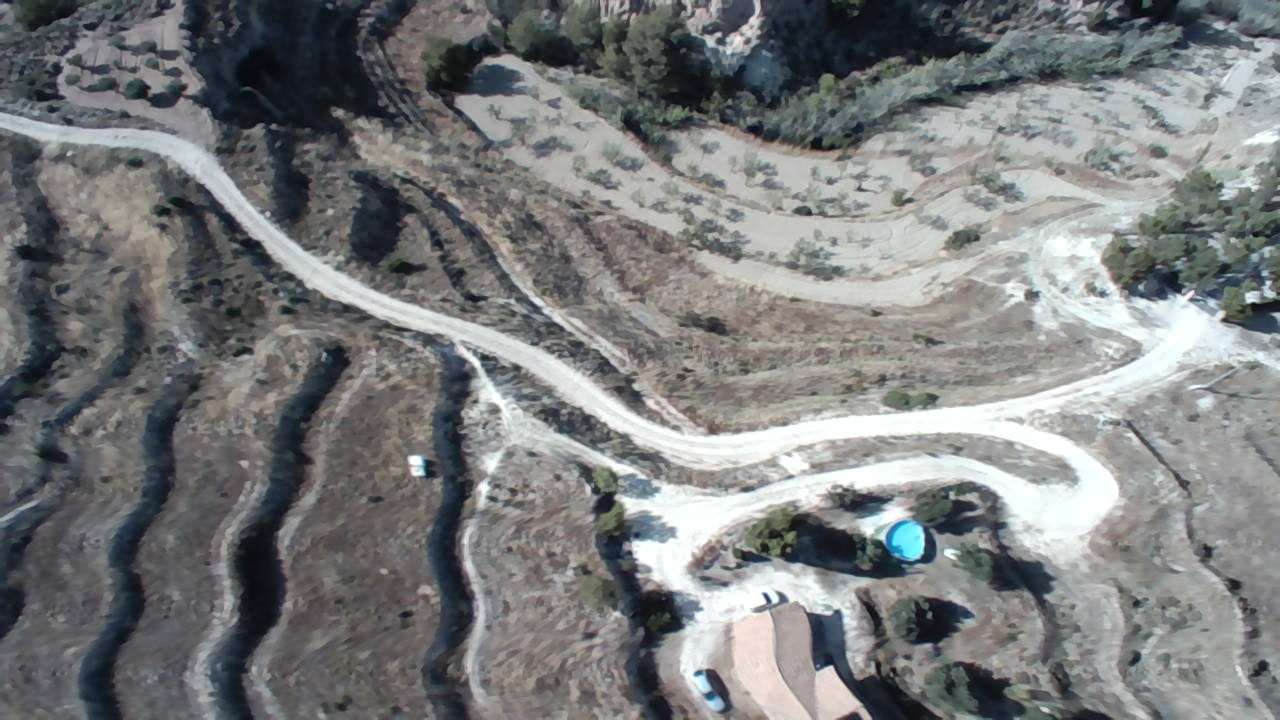
\includegraphics[width=\textwidth,height=4.5cm,keepaspectratio]{frame_camara_rolling.png}
\caption{Fotograma con obturador rodante: se aprecia la imagen ondulada por el efecto de \textit{skew}.}
\label{fig:frame-rolling}
\end{minipage}
\hfill
\begin{minipage}[b]{0.48\textwidth}
\centering
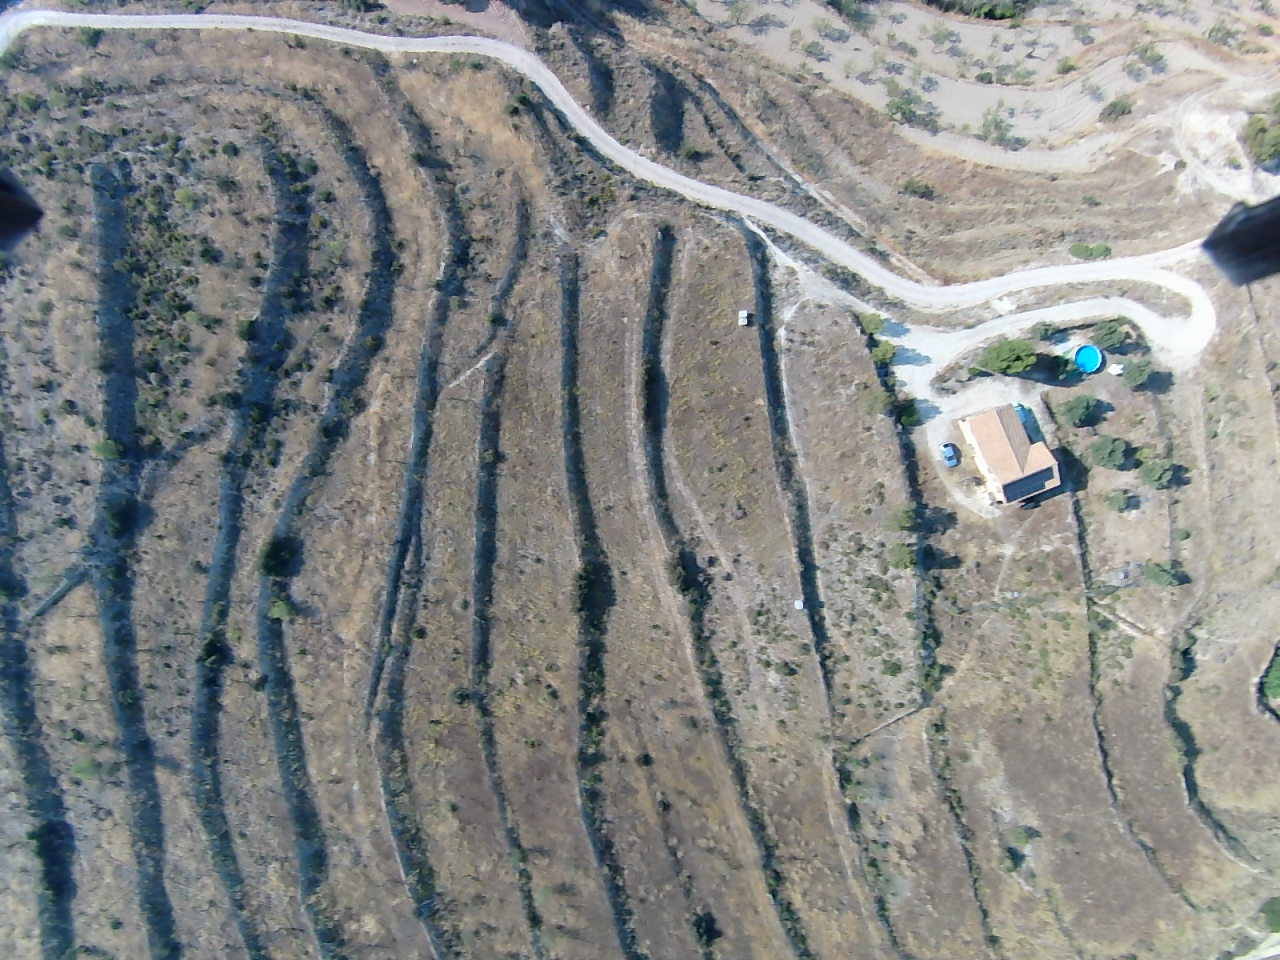
\includegraphics[width=\textwidth,height=4.5cm,keepaspectratio]{frame_camara_global.png}
\caption{Fotograma con obturador global (Svpro AR0234): sin deformación apreciable pese a las vibraciones.}
\label{fig:frame-global}
\end{minipage}
\end{figure}

\section{Conexiones eléctricas y de datos}
\label{sec:conexiones-electricas-datos}

Los conectores relevantes de la placa controladora (stack H743 6S, basada en el microcontrolador STM32H743) usados en este proyecto, ya representados en el esquema eléctrico de la \autoref{fig:alimentacion-dron}, son:

\begin{itemize}
\item \textbf{Alimentación auxiliar}: se soldó un cable directamente a los pines de entrada de batería de la FC (\texttt{BAT}/\texttt{GND}) para alimentar el BEC ajustable desde la tensión bruta de la batería, en vez de depender de una salida ya regulada de la propia FC. Esto da una línea de alimentación independiente para la Raspberry Pi, la cámara y el resto de electrónica auxiliar.
\item \textbf{Telemetría hacia la Raspberry Pi}: se cablea el puerto serie \texttt{SERIAL2} de la FC (pines \texttt{T2}/\texttt{R2}) a los pines GPIO14 (TXD, pin físico 8) y GPIO15 (RXD, pin físico 10) de la Raspberry Pi, cruzando TX y RX entre ambos dispositivos (T2$\to$RXD, R2$\to$TXD), más una referencia de masa común (GND).
\item \textbf{GPS y brújula}: el módulo GPS M10 se conecta al puerto etiquetado \texttt{GPS} de la FC (T1/R1 para UART, SDA/SCL para la brújula por I2C).
\item \textbf{Receptor de radiocontrol}: el receptor FlySky FS-i6X se conecta al puerto de recepción de la FC (protocolo iBUS), lo que permite tomar el control manual del dron mediante la emisora en cualquier momento de la misión (\autoref{sec:controlador-sensores}).
\end{itemize}

\section{Computadora de borde y comunicaciones}
\label{sec:hardware-raspberry-comunicaciones}

La Raspberry Pi actúa como computadora de borde. En la configuración actual se encarga de ejecutar el programa de captura, guardar los fotogramas y registrar la telemetría disponible. También se conecta un dongle LTE para mantener comunicación con el ordenador de tierra. Sobre esta comunicación se utiliza Tailscale (\autoref{sec:acceso-remoto}), lo que permite acceder al sistema de forma remota mediante una red privada virtual.

La Raspberry Pi empleada es una \textbf{Raspberry Pi 3B+}. Se trata de un modelo ya antiguo y limitado para las exigencias del pipeline de geolocalización visual completo: no dispone de aceleración por GPU ni de memoria suficiente para cargar simultáneamente los modelos DINOv3-vitl16 y LoFTR (\autoref{sec:analisis-rendimiento}). En este proyecto se ha usado únicamente para las tareas que sí puede asumir con margen —captura de imágenes, registro de telemetría y comunicaciones—, dejando explícitamente fuera de su alcance la ejecución a bordo del pipeline visual completo, que se evalúa en un ordenador externo con GPU (\autoref{sec:decisiones-diseno}).

\section{Pruebas de integración hardware}
\label{sec:pruebas-hardware}

La \autoref{tab:pruebas-hardware} recoge las pruebas básicas realizadas antes de los vuelos de captura, para validar la integración física de la plataforma.

\begin{table}[htbp]
\centering
\caption{Pruebas básicas de integración hardware.}
\label{tab:pruebas-hardware}
\begin{tabularx}{\textwidth}{p{0.22\textwidth}Xp{0.22\textwidth}}
\toprule
\textbf{Prueba} & \textbf{Criterio de aceptación} & \textbf{Resultado obtenido} \\
\midrule
Continuidad eléctrica & No existen cortocircuitos entre alimentación y masa. & No se detectaron cortocircuitos. \\
Regulación del BEC & La tensión de salida coincide con la requerida por la electrónica auxiliar. & El BEC entregaba correctamente \SI{5}{\volt}. \\
Orden de motores & Cada motor responde al canal correcto y gira en el sentido esperado. & El orden y sentido de giro de los cuatro motores era correcto. \\
Lectura de GPS y brújula & La estación de tierra recibe posición y rumbo coherentes. & Cumplido, tras corregir la posición y orientación del GPS (\autoref{sec:problema-gps-proximidad}, \autoref{sec:problema-brujula-invertida}). \\
Captura de cámara & La Raspberry Pi detecta la cámara y guarda imágenes sin cortes. & Cumplido: 142 fotogramas capturados de forma continua en el vuelo de validación (\autoref{sec:zona-condiciones-vuelo}). \\
Vibraciones & Las imágenes capturadas no presentan desenfoque o deformaciones severas. & No se aprecian deformaciones ni desenfoque relevantes, gracias al montaje antivibración (\autoref{sec:camara-montaje}). \\
\bottomrule
\end{tabularx}
\end{table}

\section{Problemas encontrados y soluciones}
\label{sec:problemas-hardware}

Esta sección documenta, con el formato problema\,$\rightarrow$\,diagnóstico\,$\rightarrow$\,solución, los principales incidentes de integración hardware surgidos durante el proyecto.

\subsection{Pérdida del \textit{firmware}/\textit{bootloader} de la placa de vuelo}
\label{sec:problema-stlink}

\textbf{Problema.} Al instalar ArduPilot desde la aplicación de Betaflight (subiendo directamente el archivo \texttt{.hex} del \textit{firmware}), el proceso de flasheo se interrumpió a mitad de camino y, a partir de ese momento, la placa dejó de responder por completo: ya no era detectada como dispositivo USB por el ordenador ni aparecía ningún puerto serie nuevo al conectarla, sin ningún mensaje de error claro que explicara qué había fallado.

\textbf{Diagnóstico.} El flasheo interrumpido a mitad de escritura dejó la memoria flash del microcontrolador STM32H743 (en particular, el \textit{bootloader}) en un estado corrupto o vacío, sin programa válido que ejecutar al arrancar. Sin bootloader activo la placa no puede enumerarse como dispositivo USB ni comunicarse con Mission Planner, lo que normalmente obligaría a sustituir la placa completa; sin embargo, el microcontrolador seguía físicamente intacto y accesible mediante su interfaz de depuración SWD, independiente del USB y del bootloader.

\textbf{Solución.} Se reprogramó el microcontrolador directamente por SWD con un programador \textbf{ST-Link V2}, evitando así el USB/bootloader de la propia placa y comprando únicamente el programador (mucho más barato que sustituir la FC completa). El procedimiento seguido fue:

\begin{enumerate}
\item Conexión del ST-Link V2 (\autoref{fig:swd-pads}) a cuatro pads sin serigrafiar situados junto al chip STM32H743, entre los conectores de motores \texttt{M6}/\texttt{M7}/\texttt{M8}, etiquetados en la serigrafía de la placa simplemente como \texttt{C}, \texttt{D}, \texttt{G} y \texttt{3} (\texttt{C}=SWCLK, \texttt{D}=SWDIO, \texttt{G}=GND; el pad \texttt{3}, presumiblemente 3V3, no se llegó a conectar por no ser necesario con la placa ya alimentada). Estos pads son extremadamente pequeños y fáciles de dañar: uno de ellos se desprendió de la placa al desoldar el cable del ST-Link tras terminar el procedimiento, aunque sin afectar al resultado ya obtenido.
\item Descarga del firmware de ArduCopter precompilado para el target oficial \texttt{DAKEFPVH743} del servidor de \textit{firmware} de ArduPilot, en formato \texttt{arducopter\_with\_bl.hex} (incluye el \textit{bootloader}, por lo que no hace falta flashearlo aparte).
\item Programación con \textbf{STM32CubeProgrammer} en modo automático: con el archivo \texttt{.hex} cargado (el campo de dirección de inicio se deja vacío, ya que el formato HEX incluye las direcciones de memoria embebidas, a diferencia de un \texttt{.bin}), se marcan las opciones \textit{Full chip erase}, \textit{Download file} y \textit{Verify programming}, y se ejecuta \textit{Start Programming}.
\item Verificación: tras desconectar el ST-Link y conectar la placa solo por USB, apareció un puerto COM nuevo en el sistema —señal de que el \textit{bootloader} de ArduPilot estaba de nuevo activo— y Mission Planner pudo conectar a \SI{115200}{baud} y mostrar telemetría en vivo del giroscopio.
\end{enumerate}

Tras el flasheo fue necesario repetir la configuración inicial del controlador desde cero (el chip se había borrado por completo): calibración de acelerómetro, calibración de brújula, configuración del tipo de \textit{frame} (número de motores y geometría) y calibración de radio.

\begin{figure}[htbp]
\centering
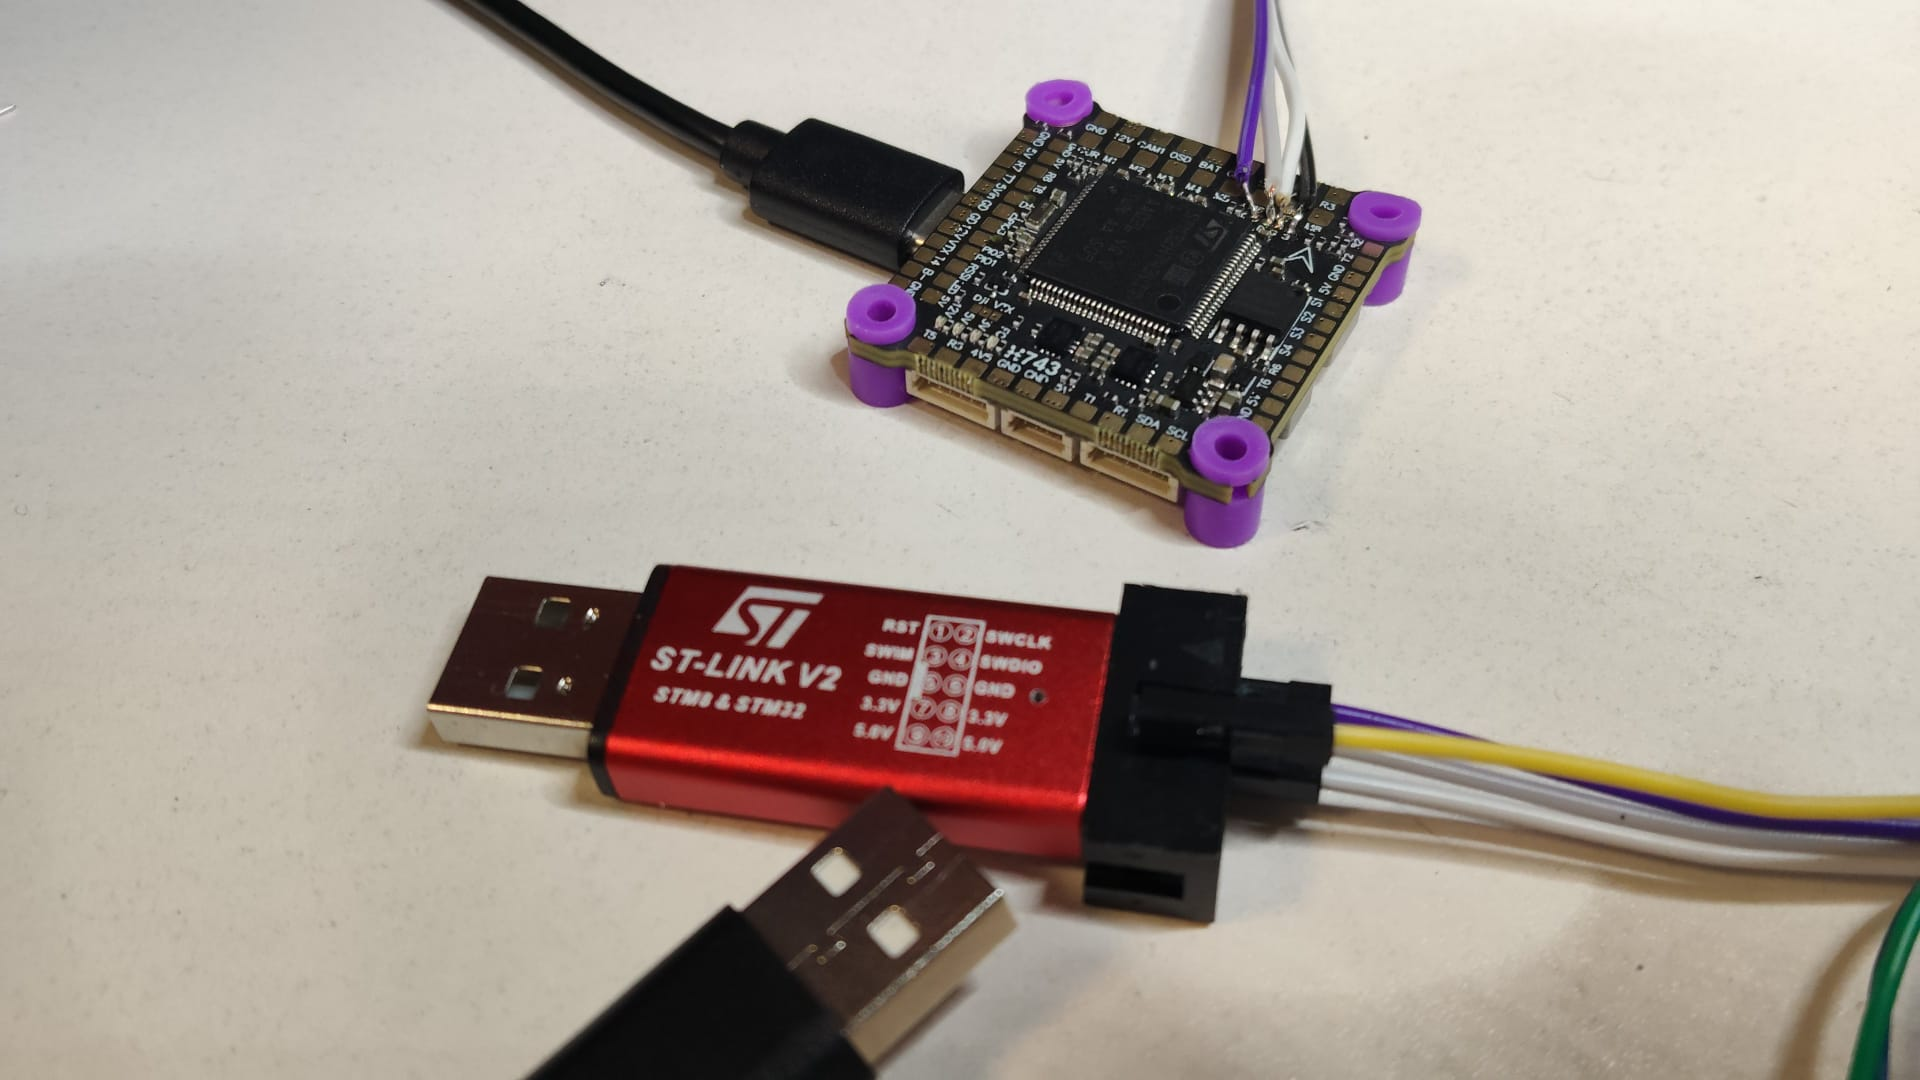
\includegraphics[width=0.7\textwidth]{soldadura_stlink.png}
\caption{ST-Link V2 conectado a los pads de depuración SWD de la FC, con los cables soldados junto a los conectores de motores M6/M7/M8.}
\label{fig:swd-pads}
\end{figure}

\subsection{Pérdida de señal GPS por proximidad a otros componentes}
\label{sec:problema-gps-proximidad}

\textbf{Problema.} Con el módulo GPS M10 anclado directamente sobre el chasis, cerca de la FC y del resto de la electrónica, el número de satélites detectados era insuficiente para obtener una posición fiable.

\textbf{Diagnóstico.} La proximidad de la antena GPS a la FC, los cables de potencia y el resto de electrónica introduce interferencia electromagnética que degrada la recepción de la señal GNSS, y además el propio chasis y los componentes montados a su alrededor reducen la porción de cielo visible para la antena.

\textbf{Solución.} Se diseñó e imprimió en 3D un mástil que eleva el módulo GPS por encima del resto de la electrónica (\autoref{sec:modelos-3d}). Tras este cambio, el número de satélites detectados fue suficiente y estable, sin más incidencias de pérdida de posición.

\subsection{Brújula invertida tras montar el mástil del GPS}
\label{sec:problema-brujula-invertida}

\textbf{Problema.} Al imprimir e instalar el mástil 3D que eleva el módulo GPS/brújula por encima del resto de la electrónica (\autoref{sec:problema-gps-proximidad}), se montó con una orientación equivocada sobre el chasis, de forma que el módulo quedó mirando hacia atrás en vez de hacia delante. En el primer vuelo de prueba tras ese montaje, el dron entró en lo que se conoce como \textit{toilet bowling} (el dron gira en círculos cada vez más amplios en vez de mantenerse estable), un síntoma característico de que el rumbo que reporta la brújula no coincide con la orientación real de la aeronave.

\textbf{Diagnóstico.} El firmware de ArduPilot asume una orientación concreta del módulo de brújula respecto al cuerpo del dron; al estar montada girada 180° respecto a esa orientación esperada, el rumbo magnético que reportaba no se correspondía con hacia dónde apuntaba realmente el dron, lo que confunde al controlador de estabilización durante el vuelo.

\textbf{Solución.} Se corrigió la orientación física del módulo GPS/brújula en el mástil para que coincidiera con la esperada por el firmware. El incidente ocurrió a poca altura, por lo que el único daño fue en las hélices (que quedaron ligeramente picadas y se sustituyeron); tras la corrección de orientación no se repitió ningún problema de sensores de la FC durante el resto de las pruebas.

No se han presentado más incidencias de sensores de la FC además de la brújula invertida.

\subsection{Calibración de la cámara}
\label{sec:referencia-problema-calibracion}

La calibración de los parámetros intrínsecos y de distorsión de la cámara se investigó como posible mejora de precisión y finalmente se descartó tras comprobarse empíricamente que no mejora el resultado; el detalle completo de este experimento se documenta junto al resto de decisiones sobre el pipeline visual, en la \autoref{sec:estado-alternativas-no-adoptadas}.

% ---------------------------------------------------------------------

% ---------------------------------------------------------------------
% Integración software
% ---------------------------------------------------------------------

\chapter{Integración software}
\label{cap:integracion-software}

\begin{Resumen}
Este capítulo describe la configuración software empleada para operar el dron, registrar datos y mantener acceso remoto. Se detallan las funciones de Mission Planner, QGroundControl, MAVProxy, Tailscale, tmux y el script de captura ejecutado en la Raspberry Pi.
\end{Resumen}

\section{Herramientas empleadas}
\label{sec:herramientas-software}

La operación del dron combina varias herramientas. Mission Planner se utiliza para configurar el controlador de vuelo, realizar calibraciones y ajustar parámetros. QGroundControl se emplea para cargar misiones de forma sencilla durante las pruebas. MAVProxy actúa como puente MAVLink entre el controlador de vuelo, la Raspberry Pi y el ordenador de tierra. Tailscale proporciona conectividad remota a través de una red privada, mientras que \texttt{tmux} permite mantener sesiones activas en la Raspberry Pi aunque se produzcan desconexiones.

\section{Enlace MAVLink}
\label{sec:enlace-mavlink}

El controlador de vuelo se conecta a la Raspberry Pi (\autoref{sec:conexiones-electricas-datos}) y expone telemetría MAVLink. MAVProxy se ejecuta en la Raspberry Pi para recibir los mensajes del controlador por dicha conexión serie y reenviarlos al ordenador de tierra mediante UDP, a través de la red Tailscale (\autoref{sec:que-es-tailscale}).

\begin{lstlisting}[language=bash,caption={Estructura del comando de reenvío MAVLink con MAVProxy.},label={lst:mavproxy}]
mavproxy.py --master=PUERTO_CONTROLADOR --baudrate 115200 \
  --out=udp:IP_PC_TAILSCALE:14550
\end{lstlisting}

\noindent donde \texttt{PUERTO\_CONTROLADOR} es el dispositivo serie de la Raspberry Pi conectado a la FC, e \texttt{IP\_PC\_TAILSCALE} es la dirección IP que Tailscale asigna al ordenador de tierra dentro de la red privada.

En el ordenador de tierra se puede abrir la estación de control escuchando el puerto UDP configurado. Esto permite visualizar telemetría durante el vuelo y facilita la depuración del sistema.

\section{Acceso remoto y ejecución persistente}
\label{sec:acceso-remoto}

\subsection{Tailscale}
\label{sec:que-es-tailscale}

Tailscale es una red privada virtual (VPN) de tipo \textit{mesh} basada en WireGuard: conecta directamente entre sí los dispositivos que forman parte de la misma red (aquí, la Raspberry Pi y el ordenador de tierra), asignándoles una dirección IP privada estable, sin necesidad de configurar manualmente un servidor VPN propio ni de abrir puertos en el router. Esto resuelve un problema concreto de este proyecto: la Raspberry Pi se conecta a internet mediante un dongle LTE, y los operadores móviles habitualmente ponen a sus clientes detrás de NAT de operador (CGNAT), por lo que la Raspberry Pi no tiene una IP pública alcanzable directamente desde el ordenador de tierra. Tailscale resuelve esto estableciendo la conexión mediante técnicas de \textit{NAT traversal} y, si no es posible una conexión directa, retransmitiendo el tráfico a través de sus propios servidores \parencite{tailscale_docs}. El resultado práctico es que, mientras la Raspberry Pi tenga cualquier tipo de acceso a internet (LTE en este caso), puede alcanzarse por SSH desde el ordenador de tierra como si estuviera en la misma red local, sin depender de la red WiFi del punto de despegue ni de configuración de red adicional.

\begin{figure}[htbp]
\centering
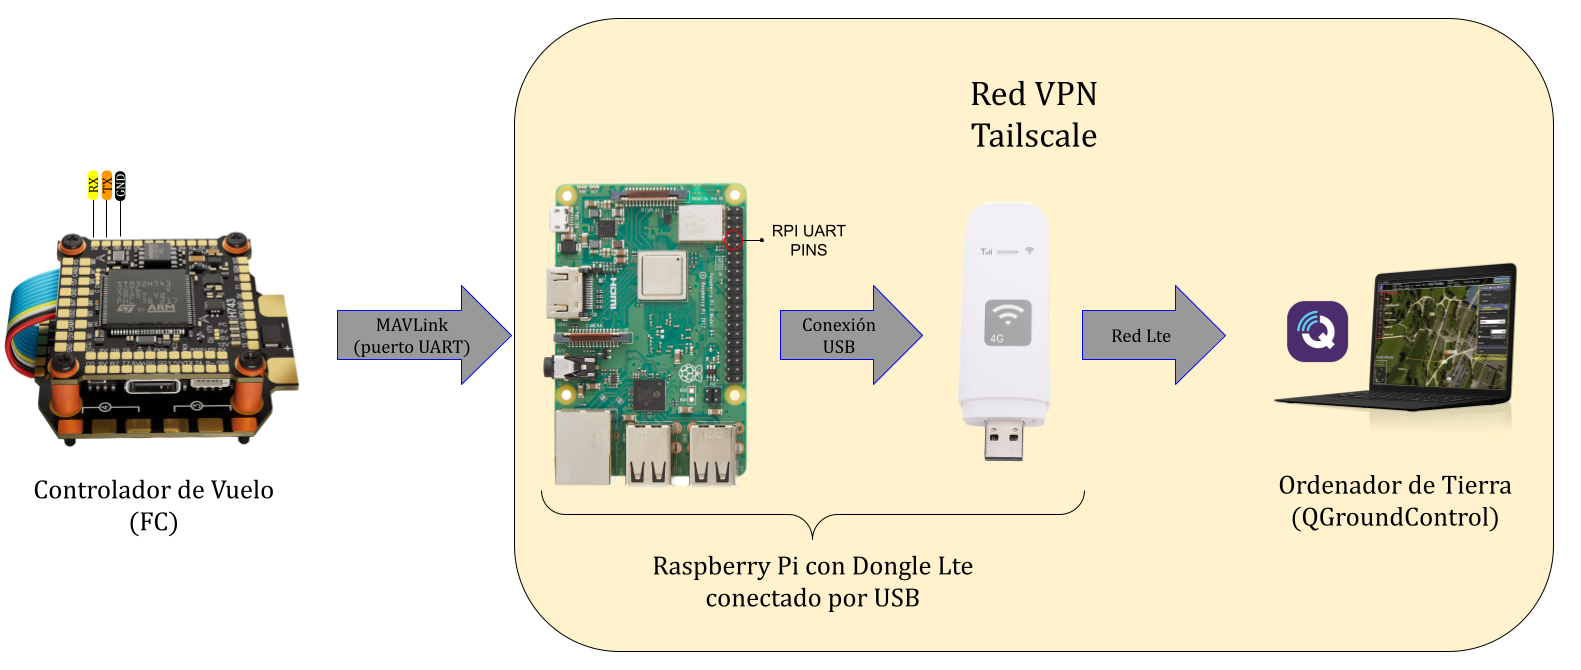
\includegraphics[width=0.9\textwidth]{camino_datos.png}
\caption{Camino de datos de telemetría desde la FC hasta el ordenador de tierra: MAVLink por UART hasta la Raspberry Pi, dongle LTE conectado por USB, red Tailscale y QGroundControl en el ordenador de tierra.}
\label{fig:diagrama-tailscale}
\end{figure}

\subsection{Sesiones persistentes con \texttt{tmux}}
\label{sec:que-es-tmux}

\texttt{tmux} es un multiplexor de terminal: permite abrir una o varias sesiones de terminal en la Raspberry Pi que siguen ejecutándose en segundo plano aunque se cierre la conexión SSH que las inició, y a las que se puede volver a acceder (\textit{reattach}) desde una conexión SSH posterior. Esto es importante porque, dependiendo de las condiciones de cobertura LTE durante un vuelo, es previsible sufrir cortes de conexión puntuales; sin \texttt{tmux}, una desconexión SSH mataría el proceso de captura (\texttt{capturar\_vuelo.py}) que se estuviera ejecutando en esa terminal, perdiendo la sesión de datos en pleno vuelo. Con el proceso de captura lanzado dentro de una sesión de \texttt{tmux}, un corte de conexión no interrumpe la captura: el proceso sigue escribiendo imágenes y telemetría en la Raspberry Pi, y basta con volver a conectar por SSH y reengancharse a la sesión (\texttt{tmux attach}) para recuperar el control y comprobar el progreso.

\section{Captura de imágenes y telemetría}
\label{sec:captura-imagenes-telemetria}

El script \texttt{capturar\_vuelo.py} implementa la captura de datos a bordo. La configuración actual establece una conexión MAVLink por UDP local, captura un fotograma cada \SI{0.5}{\second} y guarda los resultados en una carpeta de sesión. Cada sesión contiene imágenes PNG y un archivo \texttt{telemetria.csv} con el instante de captura y las variables de navegación asociadas.

\subsection{Problema de desincronización y solución con hilos independientes}
\label{sec:problema-sincronizacion-hilos}

\textbf{Problema.} En una primera versión del script de captura, la lectura del fotograma de la cámara, la lectura de la telemetría MAVLink más reciente y la escritura a disco de ambos se realizaban de forma secuencial dentro de un único bucle principal. Cuando alguna de estas operaciones tardaba más de lo esperado —en particular, la escritura de la imagen a disco—, el resto del bucle se bloqueaba esperando a que terminara, lo que introducía un retraso variable entre iteraciones. Este retraso se traducía en un desfase creciente entre el instante real de captura de cada fotograma y el instante de la fila de telemetría que se le asociaba en el CSV, un problema que se agrava con cada iteración porque el retraso se va acumulando en vez de mantenerse constante.

\textbf{Diagnóstico.} El bucle único obligaba a que la operación más lenta (escritura a disco) determinase el ritmo de todas las demás, incluida la lectura de telemetría, que en realidad no tiene motivo para depender de cuánto tarde en escribirse la imagen anterior.

\textbf{Solución.} Se separó la captura en dos hilos independientes que se ejecutan de forma concurrente: un hilo dedicado exclusivamente a leer fotogramas de la cámara y mantener siempre disponible el más reciente, y otro hilo dedicado exclusivamente a escuchar mensajes MAVLink y mantener actualizada la última telemetría recibida. El bucle principal ya no realiza directamente ninguna de las dos lecturas: en cada iteración toma el fotograma más reciente que tenga preparado el hilo de cámara, copia en el mismo instante la telemetría más reciente que tenga preparado el hilo de MAVLink, y escribe ambos a disco. De este modo, una escritura a disco lenta ya no retrasa la lectura de los siguientes fotogramas ni de la siguiente telemetría —que siguen actualizándose en sus propios hilos mientras tanto—, y el emparejamiento entre imagen y telemetría en el CSV final corresponde al mismo instante real, no a instantes progresivamente desincronizados.

\begin{table}[htbp]
\centering
\caption{Campos registrados por el script de captura.}
\label{tab:campos-telemetria}
\begin{tabularx}{\textwidth}{p{0.30\textwidth}X}
\toprule
\textbf{Campo} & \textbf{Descripción} \\
\midrule
\texttt{Timestamp} & Marca temporal usada para asociar imagen y fila de telemetría. \\
\texttt{Archivo\_Frame} & Nombre del archivo PNG guardado. \\
\texttt{Pitch}, \texttt{Roll}, \texttt{Yaw} & Actitud estimada por el controlador de vuelo. \\
\texttt{Rumbo\_Norte} & Rumbo magnético de la aeronave. \\
\texttt{Latitud}, \texttt{Longitud} & Coordenadas GNSS registradas durante el vuelo. \\
\texttt{Alt\_Relativa} & Altura relativa respecto al punto de despegue. \\
\texttt{Alt\_AMSL} & Altitud sobre el nivel medio del mar. \\
\bottomrule
\end{tabularx}
\end{table}

\section{Organización de los datos}
\label{sec:organizacion-datos}

Cada ejecución de \texttt{capturar\_vuelo.py} genera una carpeta independiente dentro del directorio de vuelos, nombrada con la fecha y hora de inicio de la sesión (por ejemplo, \texttt{vuelo\_20260716\_095840} para el vuelo de validación del \autoref{cap:experimentos-resultados}). Esta organización evita mezclar datos de distintas sesiones y facilita reproducir los experimentos sobre un vuelo concreto sin ambigüedad.

Dentro de cada carpeta de vuelo se guardan dos elementos: los fotogramas capturados, como archivos PNG nombrados con su marca temporal (\texttt{frame\_AAAAMMDD\_HHMMSS\_mmm.png}), y un único archivo \texttt{telemetria.csv} con una fila por fotograma capturado, que registra el nombre de archivo del fotograma junto con los campos descritos en la \autoref{tab:campos-telemetria} para ese mismo instante. Esta carpeta de vuelo, copiada íntegra al ordenador de procesado, es la única entrada que necesita el pipeline de geolocalización visual (\autoref{cap:geolocalizacion-visual}): a partir de ella se generan las consultas normalizadas y se evalúa el pipeline sin necesidad de ningún otro archivo de la sesión.

\section{Limitaciones actuales}
\label{sec:limitaciones-software}

La limitación principal observada es la carga computacional de la geolocalización visual. La Raspberry Pi resulta adecuada para captura y registro, pero ejecutar a bordo el pipeline completo con el descriptor VLAD+DINOv3-SAT, búsqueda en galería y emparejamiento LoFTR no es viable en la configuración actual. Por ello, la arquitectura separa la adquisición de datos en vuelo de la evaluación CVGL en un ordenador externo.

% ---------------------------------------------------------------------

% ---------------------------------------------------------------------
% Geolocalización visual
% ---------------------------------------------------------------------

\chapter{Pipeline de geolocalización visual}
\label{cap:geolocalizacion-visual}

\begin{Resumen}
Este capítulo describe el flujo de procesamiento utilizado para estimar la localización del dron a partir de imágenes: generación del mapa base, normalización de los fotogramas de vuelo, recuperación global de candidatos con un descriptor visual, verificación geométrica local y cálculo del error de localización frente a la referencia GNSS. Se documenta también qué alternativas se probaron y se descartaron en cada etapa, y por qué.
\end{Resumen}

\section{Planteamiento del problema}
\label{sec:planteamiento-cvgl}

El objetivo del pipeline es estimar la posición de una imagen capturada por el dron sin utilizar directamente su coordenada GNSS como entrada. La telemetría GNSS se conserva como referencia de evaluación, no como entrada del algoritmo. La imagen de consulta se compara con una base de datos de parches satelitales georreferenciados. Si el parche correcto se identifica y la geometría entre ambas imágenes es consistente, se puede proyectar el centro de la imagen del dron sobre el mapa y obtener una coordenada estimada.

El pipeline final se compone de las siguientes etapas, en orden: (1) generación del mapa base georreferenciado y de una galería de parches; (2) normalización de cada fotograma de vuelo (rotación a norte y ajuste de escala por altitud); (3) recuperación global de un conjunto reducido de parches candidatos mediante un descriptor visual compacto; (4) verificación geométrica local de cada candidato con emparejamiento de puntos y estimación robusta de homografía; (5) corrección del punto de verdad-terreno por la actitud del dron; y (6) cálculo del error final mediante la fórmula de Haversine. La \autoref{fig:pipeline-cvgl} resume este flujo.

\begin{figure}[htbp]
\centering
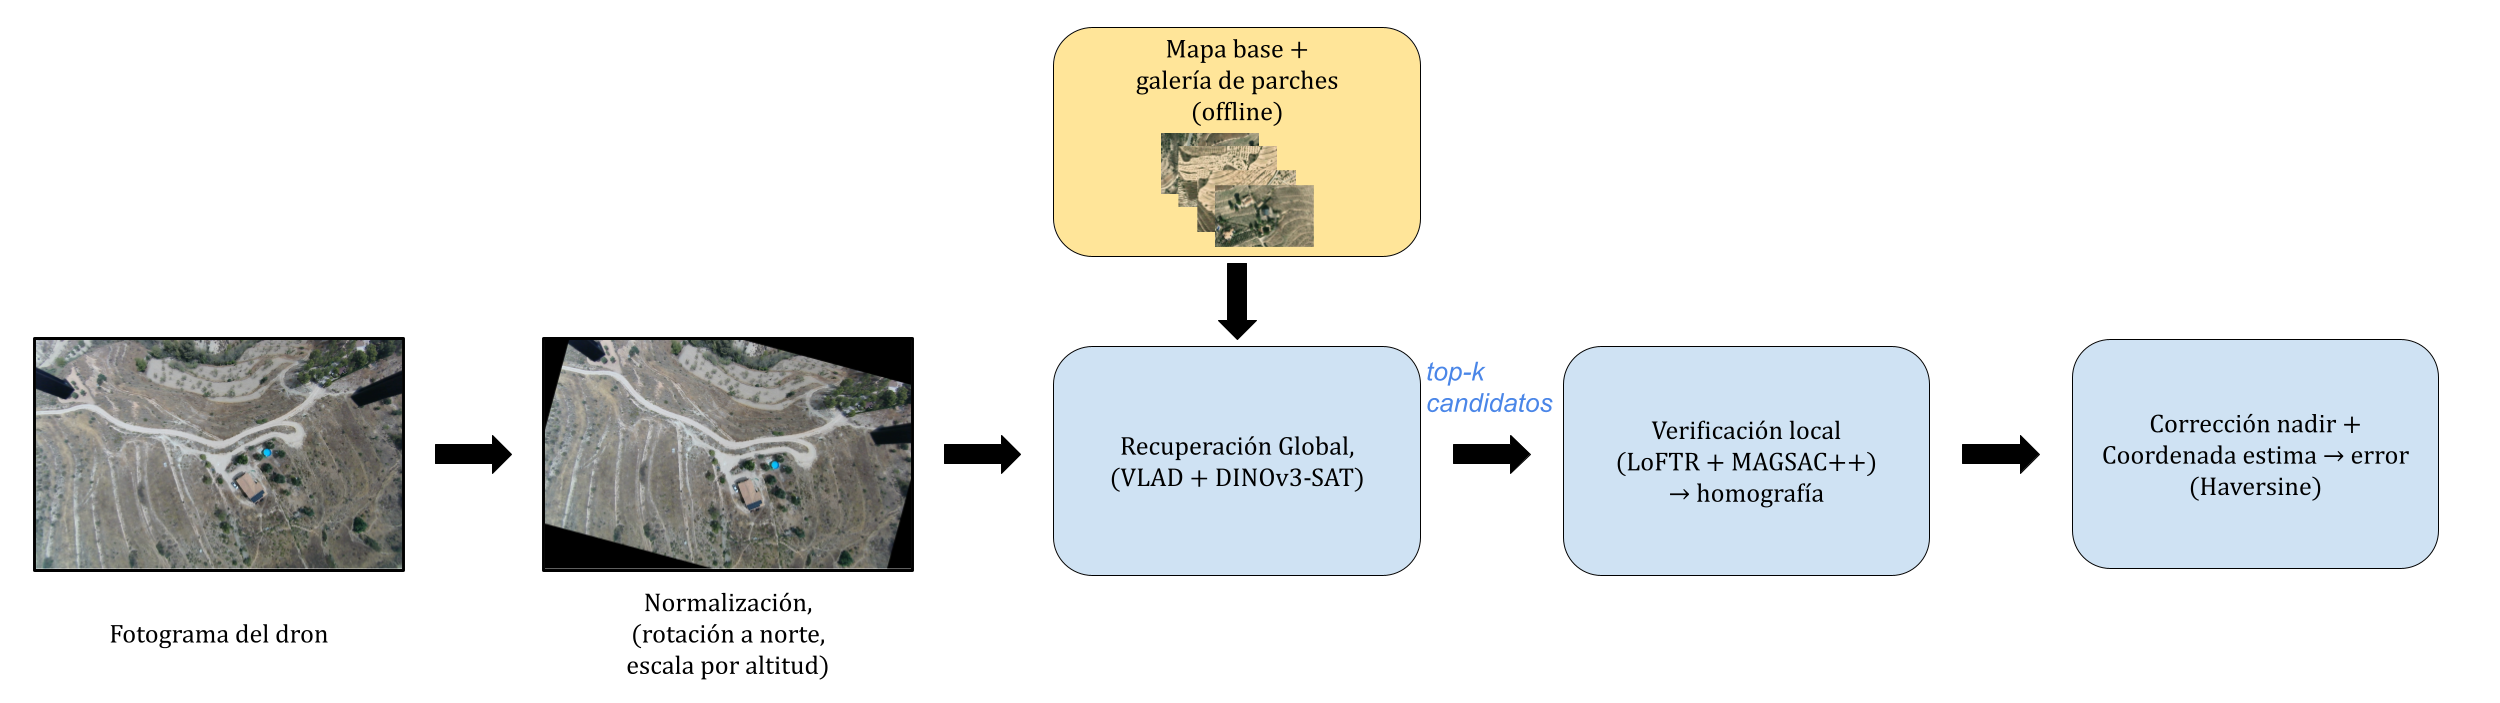
\includegraphics[width=\textwidth]{pipeline_cvgl.png}
\caption{Flujo general de geolocalización visual cruzada del pipeline final.}
\label{fig:pipeline-cvgl}
\end{figure}

\section{Generación del mapa base}
\label{sec:generacion-mapa-base}

El primer paso consiste en generar un mosaico satelital georreferenciado de la zona de vuelo. El script \texttt{01\_download\_basemap.py} descarga un área alrededor de unas coordenadas centrales (imágenes ESRI World Imagery) y la guarda como un archivo GeoTIFF en el sistema de referencia Web Mercator (EPSG:3857). Este archivo conserva la transformación entre píxeles y coordenadas proyectadas, lo que permite relacionar cada punto de la imagen con una posición geográfica.

Dos parámetros de esta descarga son configurables: el \textbf{radio} del área descargada alrededor del centro y el \textbf{nivel de zoom} (resolución de las teselas). Ambos se evaluaron empíricamente en vez de fijarse por criterio, comparando precisión de localización y tiempo de preparación sobre un subconjunto de 15 fotogramas de prueba y cuatro radios (500, 1500, 3000 y 5000 m) a zoom fijo, y tres niveles de zoom (17, 18 y 19) a radio fijo:

\begin{itemize}
\item El radio apenas afecta a la precisión (mediana de error entre 5,5 y 6,1 m en todo el rango probado), pero el coste de preparación (descarga y cálculo de descriptores de la galería) crece de forma muy rápida con el área: de unos 40 s a radio 500 m a más de 80 minutos a radio 5000 m (\autoref{fig:tiempos-setup-radio-zoom}). Se mantiene un radio de 1500 m, un compromiso razonable para el área de vuelo de las pruebas.
\item El nivel de zoom 18 (el adoptado) obtiene la mejor mediana de error; el zoom 17 (menor resolución) produjo dos fallos catastróficos de más de 800 m en el mismo conjunto de prueba —casos en los que el emparejamiento local no encontró suficientes puntos fiables—, mientras que el zoom 19 no mejora la precisión pero duplica el tiempo por consulta y multiplica por 15 el tiempo de descarga.
\end{itemize}

\begin{figure}[htbp]
\centering
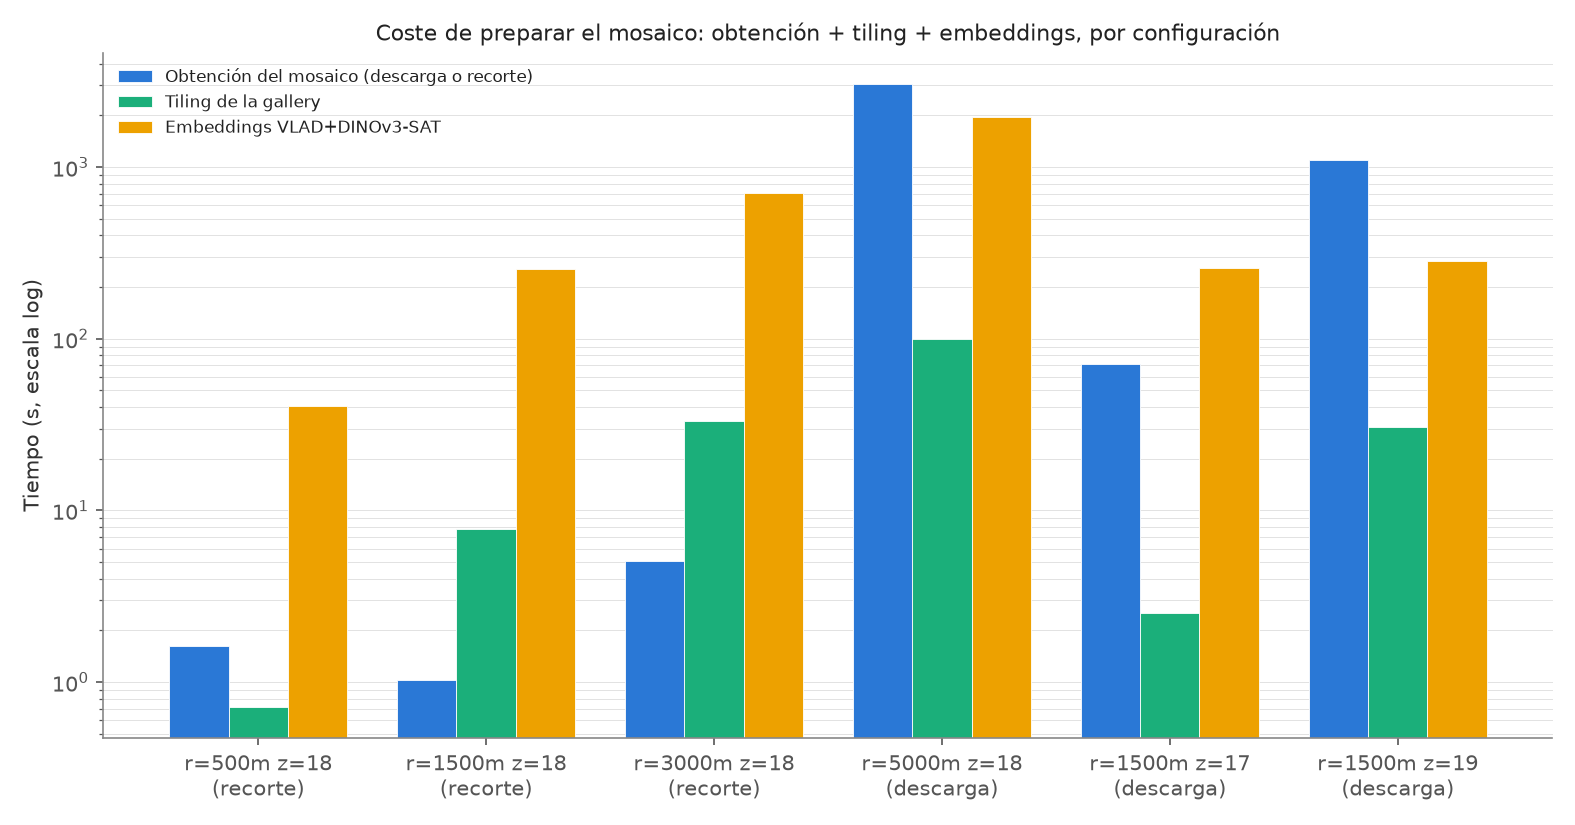
\includegraphics[width=0.85\textwidth]{tiempos_setup_radio_zoom.png}
\caption{Tiempo de obtención del mosaico, tiling de la galería y cálculo de embeddings, para las seis configuraciones de radio/zoom evaluadas (escala logarítmica).}
\label{fig:tiempos-setup-radio-zoom}
\end{figure}

\section{Normalización de los fotogramas de vuelo}
\label{sec:normalizacion-frames}

Antes de comparar un fotograma del dron con la galería satelital es necesario corregir dos desajustes que, de no tratarse, degradan gravemente el emparejamiento:

\begin{description}
\item[Rotación a norte.] El mosaico satelital está orientado con el norte geográfico hacia arriba, pero el fotograma del dron está orientado según el rumbo de vuelo en el instante de captura. El script \texttt{10\_preparar\_queries\_vuelo\_completo.py} rota cada fotograma según el campo \texttt{Rumbo\_Norte} de la telemetría para que \enquote{arriba} apunte siempre al norte, igual que la galería. Sin esta corrección, el número de \textit{inliers} geométricos encontrados por LoFTR cae de cientos (en fotogramas ya alineados a norte) a menos de una decena en fotogramas girados 90--180° respecto al norte, es decir, se pierde el emparejamiento casi por completo salvo cuando el rumbo del dron coincide por casualidad con el norte.
\item[Normalización de altitud.] Tanto el descriptor global como el emparejador local redimensionan internamente la imagen a un tamaño de entrada fijo, con independencia del tamaño real de entrada. Si un fotograma se capturó a más altitud que la altitud de referencia usada para dimensionar los parches de la galería, cubre más terreno real que dichos parches, y el mismo objeto del mundo real aparece a una escala de píxeles distinta en la consulta que en el parche. El mismo script corrige esto recortando al centro la fracción de la imagen que cubriría la altitud de referencia (80 m en este proyecto), en vez de reescalar la imagen completa, ya que el redimensionado final es fijo de todas formas.
\end{description}

\section{Construcción de la galería satelital}
\label{sec:construccion-galeria}

El script \texttt{02\_tile\_basemap\_gallery.py} divide el mapa base en parches con solapamiento del 30\,\%. Cada parche se guarda como imagen PNG y se registra en un CSV con su coordenada central y su posición dentro del mosaico original. El tamaño de los parches se calcula a partir de una estimación de la huella de la cámara en el suelo.

La anchura aproximada de terreno observada por una cámara nadiral puede estimarse mediante:

\begin{equation}
W = 2h \tan\left(\frac{\theta}{2}\right)
\label{eq:huella-camara}
\end{equation}

\noindent donde $W$ es la anchura de la huella en metros, $h$ es la altura relativa de vuelo y $\theta$ es el campo de visión horizontal (HFOV) efectivo de la cámara. Este HFOV efectivo (\ang{121} en la configuración final, para el sensor AR0234 en modo 1920$\times$1200) no es el nominal de la lente, sino un valor calibrado empíricamente: se midió sobre imágenes reales la anchura de terreno cubierta a dos alturas de vuelo muy distintas (80 m y 120 m) y se comprobó que ambas mediciones eran consistentes entre sí con la \autoref{eq:huella-camara}. Esta huella, además, se calcula en metros reales de terreno y debe convertirse a \enquote{metros proyectados} del mosaico Web Mercator multiplicando por el factor de escala local $\sec(\mathrm{lat})$, ya que dicha proyección solo preserva distancias reales en el ecuador; omitir este factor infraestima el tamaño de parche necesario a las latitudes de este proyecto (unos 38--39° N).

\section{Recuperación global}
\label{sec:recuperacion-global}

La recuperación global busca rápidamente los parches satelitales más parecidos a la imagen del dron, para reducir el problema de \enquote{buscar en toda la galería} a \enquote{verificar geométricamente un puñado de candidatos}. Para ello se calcula un descriptor visual compacto de cada parche de la galería (una sola vez, cacheado) y de cada consulta, y se ordenan los parches por similitud coseno.

\subsection{Configuración final: VLAD + DINOv3-SAT}
\label{sec:recuperacion-global-final}

La configuración inicialmente prevista, siguiendo el enfoque más simple de AnyLoc \parencite{keetha2023anyloc}, era un descriptor DINOv2 con agregación GeM (\textit{Generalized Mean pooling}). Evaluada sobre las 76 consultas del vuelo de validación, esta configuración obtenía una posición mediana del parche correcto en el puesto 13 del ranking global y una tasa de acierto en primera posición (\textit{top-1}) del 0\,\%: la fase de recuperación global casi nunca encontraba el parche correcto como mejor candidato.

En vez de dar por buena esta configuración, se compararon empíricamente 2 esquemas de agregación (GeM y VLAD) por 3 backbones (DINOv2, DINOv3-vitb16 preentrenado en imágenes web genéricas, y DINOv3-vitl16 preentrenado específicamente en imágenes de satélite, variante SAT-493M), es decir, 6 combinaciones sobre las mismas 76 consultas y la misma galería. La \autoref{fig:comparacion-retrieval} resume el resultado.

\begin{figure}[htbp]
\centering
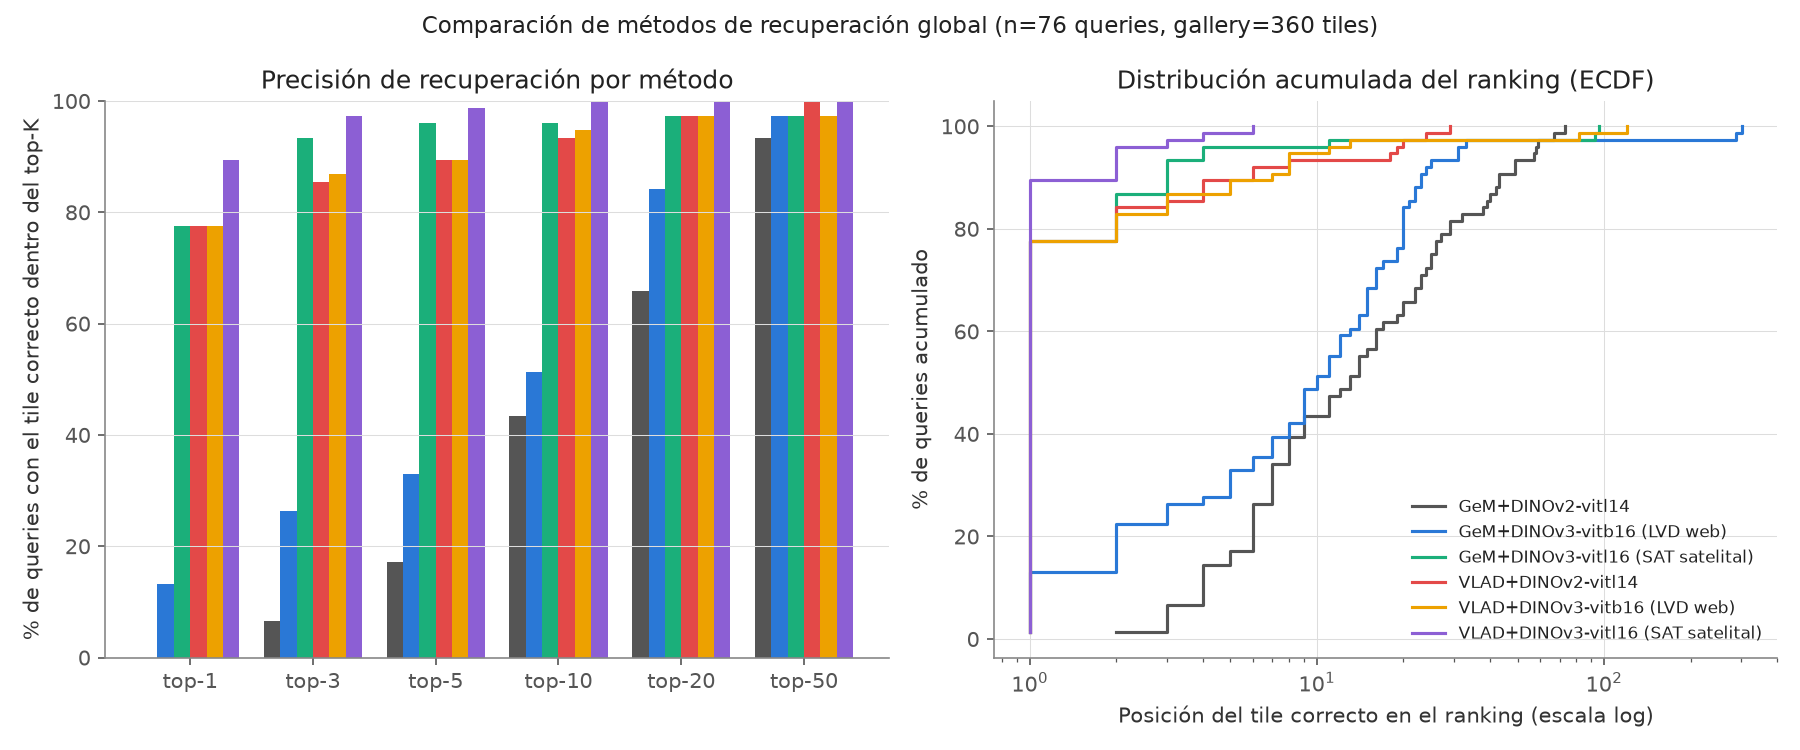
\includegraphics[width=\textwidth]{comparacion_retrieval_metodos.png}
\caption{Comparación de las 6 combinaciones de agregación (GeM/VLAD) y backbone (DINOv2/DINOv3-LVD/DINOv3-SAT) evaluadas para la recuperación global.}
\label{fig:comparacion-retrieval}
\end{figure}

La combinación ganadora, VLAD con DINOv3-vitl16 (variante SAT-493M), obtiene una posición mediana del parche correcto de 1 (top-1 = 89,5\,\%, top-5 = 98,7\,\%, top-10 = 100\,\%). Dos factores explican esta mejora:

\begin{itemize}
\item \textbf{VLAD frente a GeM}: VLAD (\textit{Vector of Locally Aggregated Descriptors}) ajusta un vocabulario visual mediante \textit{k-means} sobre los propios parches de la galería y agrega los tokens de cada imagen como residuos respecto a ese vocabulario \parencite{arandjelovic2016netvlad}, en vez de promediar directamente los tokens como hace GeM. Esto preserva más información local sobre qué elementos visuales aparecen en la imagen, en vez de reducirlos a un único promedio global.
\item \textbf{DINOv3-SAT frente a DINOv2}: la variante SAT-493M de DINOv3 está preentrenada específicamente sobre imágenes de satélite \parencite{simeoni2025dinov3}. Aunque el dominio \enquote{vista de dron} no está cubierto por ese preentrenamiento, la galería contra la que se compara es, precisamente, satelital, por lo que comparte mucha más estructura visual con el backbone que un modelo entrenado sobre fotografía web genérica.
\end{itemize}

Con esta mejora en la calidad del ranking, la mayoría de consultas resuelven correctamente con un único candidato, lo que permite aplicar una parada temprana (\textit{early-exit}) en la fase de emparejamiento local: en cuanto un candidato supera un umbral de correspondencias geométricamente consistentes, se descarta el resto del top-k sin evaluarlo. Esta optimización, combinada con precisión de cálculo reducida (FP16) y un tamaño de imagen de entrada más pequeño para LoFTR, se describe con sus tiempos en la \autoref{sec:emparejamiento-local}.

\section{Emparejamiento local y estimación geométrica}
\label{sec:emparejamiento-local}

La fase local compara la imagen del dron con cada candidato del top-k utilizando LoFTR (\textit{Local Feature TRansformer}) \parencite{sun2021loftr}, un emparejador \textbf{sin detector} de puntos de interés: en vez de extraer primero un conjunto reducido de puntos clave y describirlos por separado (como SIFT u ORB), LoFTR predice directamente correspondencias densas entre las dos imágenes mediante un transformador con atención cruzada. Se eligió este enfoque frente a los detectores clásicos porque las escenas de este proyecto (terreno agrícola/forestal, visto desde ángulos y alturas muy distintos entre dron y satélite) presentan zonas de textura repetitiva o baja, donde los detectores de esquinas clásicos tienden a fallar o a producir puntos poco distintivos.

Las correspondencias que produce LoFTR se filtran primero por confianza y después se ajusta una homografía robusta con MAGSAC++ \parencite{barath2020magsac++}, una variante de RANSAC que no necesita fijar a mano un único umbral de error para clasificar una correspondencia como \textit{inlier}, sino que marginaliza sobre un rango de umbrales, lo que la hace más estable cuando la proporción de correspondencias erróneas varía mucho de una imagen a otra (como ocurre al comparar candidatos de calidad muy distinta dentro del top-k). El candidato con mayor número de \textit{inliers} se considera la mejor hipótesis de localización, y su homografía se usa para proyectar el centro de la imagen del dron sobre el mosaico satelital. A partir del píxel proyectado se obtiene una coordenada geográfica con las utilidades de conversión de \texttt{geo\_utils.py}. El script \texttt{11\_ejecutar\_vuelo\_completo.py} implementa esta etapa sobre el pipeline completo.

\subsection{Optimización del tiempo de emparejamiento}
\label{sec:optimizacion-loftr}

LoFTR es la etapa más costosa del pipeline por candidato evaluado, por lo que se aplicaron tres optimizaciones, validadas empíricamente comparando tiempo y precisión antes/después de cada una:

\begin{itemize}
\item \textbf{Early-exit}: se detiene la evaluación de candidatos del top-k en cuanto uno supera un umbral de \textit{inliers} (100), en vez de evaluar siempre los 20 candidatos. Gracias a la buena calidad del ranking (\autoref{sec:recuperacion-global-final}), la mayoría de consultas resuelven con un único candidato evaluado.
\item \textbf{Precisión FP16}: LoFTR se ejecuta en punto flotante de 16 bits en GPU en vez de 32 bits, reduciendo tiempo de cálculo y memoria sin pérdida apreciable de precisión de localización.
\item \textbf{Tamaño de imagen reducido} (\texttt{MAX\_SIDE=384} en vez de 640): las imágenes de entrada a LoFTR se redimensionan a un lado máximo menor antes del emparejamiento.
\end{itemize}

Sobre las 76 consultas del vuelo de validación, la combinación de las tres optimizaciones reduce el tiempo medio por consulta a unos 0,3--0,4 s (frente a varios segundos sin optimizar), de los cuales aproximadamente dos tercios corresponden a la extracción del descriptor global VLAD+DINOv3-SAT y un tercio al emparejamiento LoFTR (\autoref{fig:tiempo-desglose}) — es decir, en la configuración final el cuello de botella ya no es LoFTR, sino la extracción del descriptor de recuperación global.

\begin{figure}[htbp]
\centering

\includegraphics[width=0.9\textwidth]{tiempo_desglose.png}
\caption{Desglose del tiempo por consulta entre recuperación global (VLAD+DINOv3-SAT) y emparejamiento local (LoFTR+MAGSAC++), a lo largo de las 76 consultas del vuelo de validación.}
\label{fig:tiempo-desglose}
\end{figure}

Se evaluaron además dos alternativas que \textbf{no} se adoptaron en la versión final, a pesar de probarse con el mismo rigor que las anteriores: procesar varios pares candidato-consulta en el mismo lote de LoFTR (\textit{batching}), que ofrecía una mejora de tiempo modesta a cambio de mayor riesgo de agotar memoria de GPU; y EfficientLoFTR, una variante más ligera de LoFTR que en la práctica no superó al LoFTR ya optimizado con las tres técnicas anteriores.

\section{Corrección del punto de verdad-terreno}
\label{sec:correccion-nadir}

La telemetría GNSS registra la posición de la antena/IMU del dron, no la del punto de terreno que realmente fotografía el centro de la cámara. Con \textit{pitch} y \textit{roll} nulos ambos puntos coinciden, pero en vuelo real el dron cabecea y alabea para acelerar y girar, y como la cámara está montada rígidamente al cuerpo (sin estabilización por \textit{gimbal}), su eje óptico se inclina junto con el cuerpo del dron. El punto de terreno que realmente ve el centro de la imagen se desplaza respecto a la posición GNSS en la misma dirección y magnitud que esa inclinación.

Este desplazamiento en el plano del terreno, en componentes norte/este, se calcula a partir del \textit{pitch} ($\theta$), \textit{roll} ($\phi$), rumbo ($\psi$) y altura relativa ($h$) del dron en el instante de captura, aplicando la composición de rotaciones del cuerpo del dron a un vector que apunta hacia abajo en el sistema del cuerpo, y proyectando su intersección con el plano del terreno:

\begin{equation}
\begin{aligned}
N &= h \cdot \frac{\cos\psi \sin\theta \cos\phi + \sin\psi \sin\phi}{\cos\theta \cos\phi} \\
E &= h \cdot \frac{\sin\psi \sin\theta \cos\phi - \cos\psi \sin\phi}{\cos\theta \cos\phi}
\end{aligned}
\label{eq:nadir-offset}
\end{equation}

\noindent donde $N$ y $E$ son los desplazamientos en metros hacia el norte y el este que hay que sumar a la posición GNSS para obtener el punto de terreno real que mira el centro de la imagen. El signo de esta corrección se verificó empíricamente barriendo ambos signos posibles y comprobando cuál reducía el error de localización medido, no derivándolo a mano por ser propenso a errores de convenio de signos.

Aplicar esta corrección al punto de referencia usado para medir el error (en vez de comparar directamente contra la posición GNSS cruda) reduce el error medio de localización de 12,3 m a 6,2 m sobre las 76 consultas del vuelo de validación (\autoref{sec:resultados-recuperacion-global}): gran parte de lo que a primera vista parecía \enquote{error de matching} del pipeline visual no era un fallo de la recuperación o el emparejamiento, sino que se estaba comparando contra el punto de referencia equivocado.

\section{Cálculo del error}
\label{sec:calculo-error}

El error de localización se calcula comparando la coordenada estimada por visión con la coordenada de referencia (GNSS corregida por la \autoref{eq:nadir-offset}) registrada en el instante de captura, mediante la fórmula de Haversine. Esta fórmula da la distancia de gran círculo entre dos puntos de una esfera a partir de su latitud y longitud, y es la habitual para medir distancias entre coordenadas WGS84 a escala local (donde la curvatura terrestre es prácticamente despreciable pero conviene no asumir directamente una proyección plana):

\begin{equation}
d = 2R \arcsin\left(\sqrt{\sin^2\left(\frac{\Delta\varphi}{2}\right) + \cos\varphi_1 \cos\varphi_2 \sin^2\left(\frac{\Delta\lambda}{2}\right)}\right)
\label{eq:haversine}
\end{equation}

\noindent donde $\varphi_1,\varphi_2$ son las latitudes de ambos puntos, $\Delta\varphi = \varphi_2-\varphi_1$, $\Delta\lambda$ es la diferencia de longitud, y $R \approx \SI{6371}{\kilo\metre}$ es el radio medio de la Tierra. Esta métrica se calcula para cada fotograma evaluado y permite tanto reportar un error agregado (mediana, media) como analizar su distribución completa y sus casos atípicos (\autoref{sec:resultados-recuperacion-global}).

\section{Diagnóstico visual}
\label{sec:diagnostico-visual}

El script \texttt{05\_visualize\_matches.py} genera imágenes de diagnóstico para inspeccionar visualmente el comportamiento del pipeline. Una imagen muestra las correspondencias entre el fotograma del dron y el parche satelital seleccionado, diferenciando en verde los \textit{inliers} que sobrevivieron a MAGSAC++ y en rojo los descartados como \textit{outliers} (\autoref{fig:diagnostico-matches}). Otra imagen sitúa la posición GNSS real y la posición estimada sobre un recorte del mapa base, con la distancia entre ambas (\autoref{fig:diagnostico-localizacion}). Estos diagnósticos son útiles para detectar fallos de recuperación, errores de orientación, baja textura o problemas de escala que un número agregado de error no deja ver.

\begin{figure}[htbp]
\centering
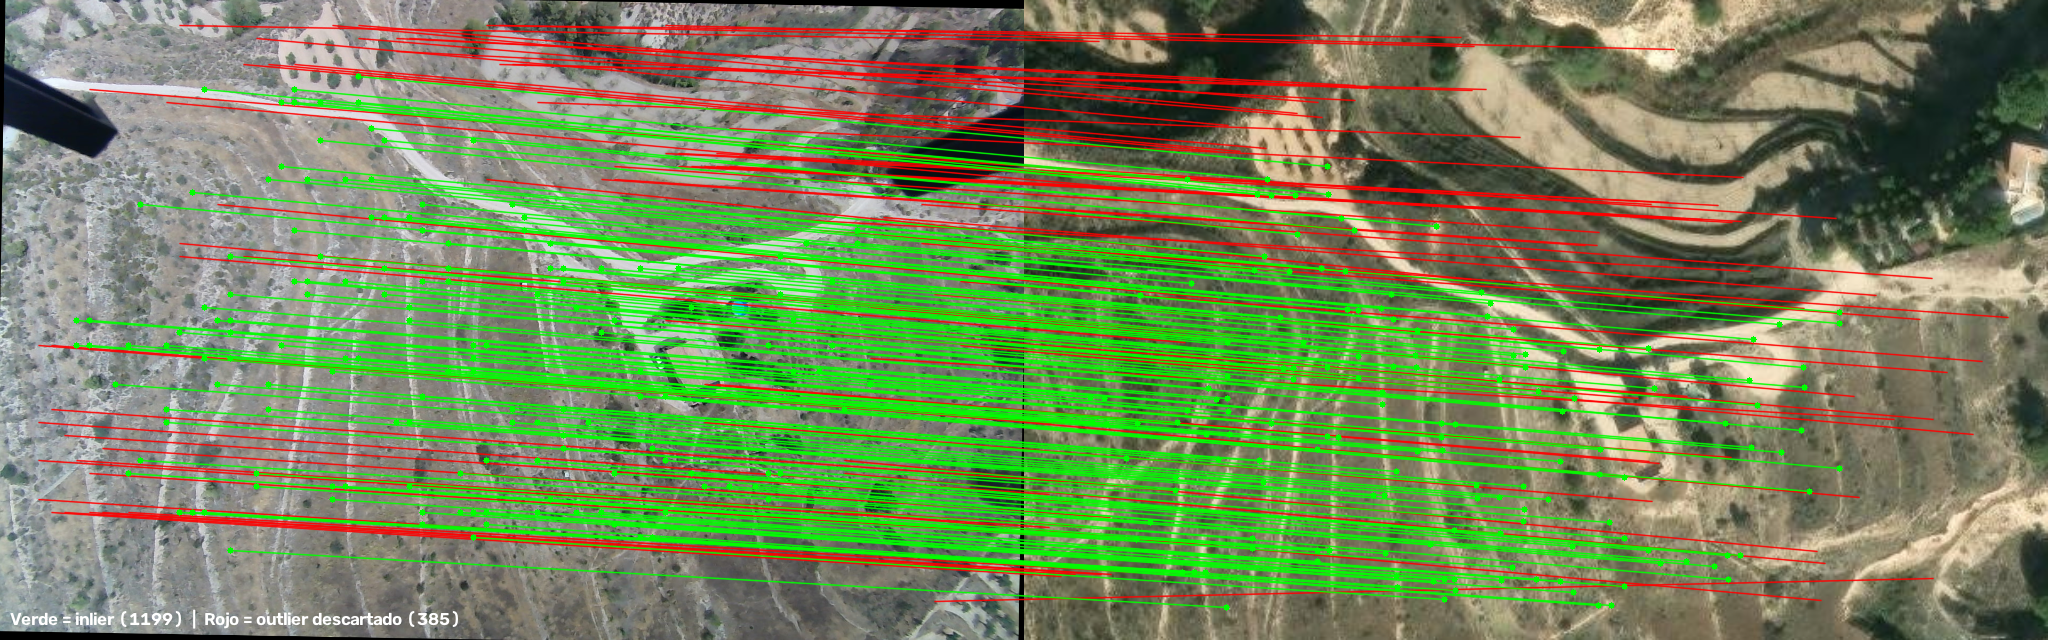
\includegraphics[width=\textwidth]{matches_ejemplo.png}
\caption{Correspondencias entre un fotograma del dron (izquierda) y el parche satelital ganador (derecha): 1199 \textit{inliers} verdes tras MAGSAC++, frente a 385 \textit{outliers} rojos descartados (el script de diagnóstico dibuja como máximo 150 líneas de \textit{inliers} y 75 de \textit{outliers}, muestreadas al azar, para no saturar visualmente la imagen; los recuentos indicados sí son el total real). Error de localización de este fotograma: 3,6 m.}
\label{fig:diagnostico-matches}
\end{figure}

\begin{figure}[htbp]
\centering
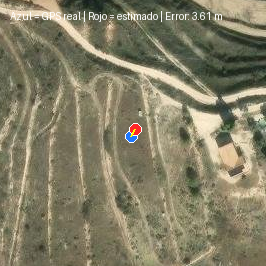
\includegraphics[width=0.55\textwidth]{location_ejemplo.png}
\caption{Comparación entre la posición GNSS real (azul) y la posición estimada por el pipeline (rojo) sobre el mosaico satelital, para el mismo fotograma de la \autoref{fig:diagnostico-matches}.}
\label{fig:diagnostico-localizacion}
\end{figure}

\section{Diagnóstico del ranking}
\label{sec:diagnostico-ranking}

El script \texttt{06\_diagnose\_retrieval\_rank.py} (en la carpeta de experimentación \texttt{pruebas/}) comprueba en qué posición del ranking global aparece el parche geográficamente correcto, utilizando la coordenada GNSS como referencia. Esta comprobación permite diferenciar dos tipos de fallo: que el parche correcto no entre en el top-k de recuperación global (fallo de recuperación), o que entre en el top-k pero la verificación local no consiga una homografía fiable (fallo de emparejamiento). Este mismo script, ejecutado sobre las 6 combinaciones de agregación/backbone, es el que produjo la comparación de la \autoref{fig:comparacion-retrieval}.

% ---------------------------------------------------------------------


% ---------------------------------------------------------------------
% Experimentos y resultados
% ---------------------------------------------------------------------

\chapter{Experimentos y resultados}
\label{cap:experimentos-resultados}

\begin{Resumen}
Este capítulo documenta el vuelo real usado para validar el pipeline de geolocalización visual, el conjunto de datos capturado, y los resultados de precisión y rendimiento obtenidos: comparación de descriptores de recuperación global, efecto de la corrección del punto de verdad-terreno, efecto de la altitud de vuelo, desglose de tiempos, y el barrido de parámetros del mosaico de referencia.
\end{Resumen}

\section{Plan experimental}
\label{sec:plan-experimental}

Los experimentos se plantearon en tres fases. La primera fase validó el funcionamiento del dron y la captura sincronizada de imágenes y telemetría en tierra y en vuelos cortos. La segunda fase realizó un vuelo controlado y georreferenciado destinado a la adquisición de datos para las pruebas del pipeline. La tercera fase ejecutó el pipeline de CVGL sobre las imágenes capturadas y comparó las posiciones estimadas con la referencia GNSS corregida (\autoref{sec:correccion-nadir}).

\section{Zona y condiciones de vuelo}
\label{sec:zona-condiciones-vuelo}

El vuelo de validación se realizó el 16 de julio de 2026. Por razones de privacidad, no se indican las coordenadas exactas de la zona; se trata de un terreno rural con bancales, de vegetación escasa y bastante seca y repetitiva a lo largo de toda la zona de vuelo. La captura comenzó a las 09:58:43 y finalizó a las 10:03:59, con una duración total de 5 minutos y 16 segundos.

\begin{table}[htbp]
\centering
\caption{Resumen del vuelo de validación.}
\label{tab:sesiones-vuelo}
\begin{tabularx}{\textwidth}{>{\bfseries}p{0.30\textwidth}X}
\toprule
\textbf{Campo} & \textbf{Valor} \\
\midrule
Fecha & 16 de julio de 2026 \\
Duración & 5 min 16 s \\
Fotogramas capturados & 142 \\
Frecuencia media de captura & 0,45 Hz ($\approx$ 1 fotograma cada 2,2 s) \\
Rango de altitud relativa & de despegue/aterrizaje ($\approx$ 0 m) hasta 120,2 m \\
Fotogramas usados como consulta (altitud $>$ 60 m) & 76 \\
\bottomrule
\end{tabularx}
\end{table}

La frecuencia de captura medida (\SI{0.45}{\hertz}, un fotograma cada $\approx$\SI{2.2}{\second}) es notablemente menor que el intervalo nominal de \SI{0.5}{\second} configurado en \texttt{INTERVALO\_SEG} (\texttt{capturar\_vuelo.py}, \autoref{sec:captura-imagenes-telemetria}). Esta diferencia se debe a la limitación de cómputo de la Raspberry Pi 3B+: escribir a disco cada fotograma PNG a la resolución nativa del sensor (1920$\times$1200) tarda por sí solo más que los \SI{0.5}{\second} configurados, por lo que el ritmo efectivo de captura queda determinado por el tiempo de escritura a disco, no por \texttt{INTERVALO\_SEG}. Esto no compromete la validez de los datos: los hilos independientes de cámara y telemetría (\autoref{sec:problema-sincronizacion-hilos}) garantizan que, aunque el ritmo de captura sea más lento de lo previsto, cada fotograma guardado sigue asociado a la telemetría de su mismo instante real.

De los 142 fotogramas capturados, se descartan los de altitud inferior a 60 m (despegue, aterrizaje y maniobras a baja altura) porque a esa altura el terreno cubierto por la cámara es demasiado pequeño para ser representativo de la galería satelital construida, quedando 76 fotogramas como consultas de evaluación.

\section{Métricas de evaluación}
\label{sec:metricas-evaluacion}

Las métricas usadas para evaluar el sistema son:

\begin{itemize}
\item \textbf{Rank de recuperación global}: posición del parche geográficamente correcto dentro del \textit{ranking} de similitud completo (no solo el top-k), y porcentaje de consultas con el parche correcto dentro del top-1/top-5/top-10.
\item \textbf{Número de \textit{inliers}}: correspondencias geométricamente consistentes tras MAGSAC++, para el mejor candidato de cada consulta.
\item \textbf{Error de localización}: distancia de Haversine (\autoref{eq:haversine}) entre la posición estimada por homografía y la coordenada GNSS de referencia, calculada tanto sin corregir (\textit{bruto}, contra la posición GNSS cruda) como corregida por la actitud del dron (\autoref{sec:correccion-nadir}).
\item \textbf{Tiempo de procesamiento por consulta}: desglosado entre extracción de descriptor global y emparejamiento local, con y sin las optimizaciones de la \autoref{sec:optimizacion-loftr}.
\end{itemize}

\section{Resultados de recuperación global}
\label{sec:resultados-recuperacion-global}

La \autoref{tab:resultados-global} resume los resultados de recuperación global para las 6 combinaciones de agregación (GeM/VLAD) y backbone (DINOv2, DINOv3-vitb16 LVD, DINOv3-vitl16 SAT) evaluadas sobre las mismas 76 consultas y la misma galería de 360 parches (ver también la \autoref{fig:comparacion-retrieval} del \autoref{cap:geolocalizacion-visual}).

\begin{table}[htbp]
\centering
\caption{Resultados de recuperación global por método (n=76 consultas, galería de 360 parches).}
\label{tab:resultados-global}
\begin{tabularx}{\textwidth}{Xp{0.13\textwidth}p{0.13\textwidth}p{0.11\textwidth}p{0.11\textwidth}p{0.12\textwidth}}
\toprule
\textbf{Método} & \textbf{Rank mediana} & \textbf{Rank media} & \textbf{Top-1} & \textbf{Top-5} & \textbf{Top-10} \\
\midrule
GeM + DINOv2-vitl14           & 13 & 18,9 & 0,0\%   & 17,1\% & 43,4\% \\
GeM + DINOv3-vitb16 (LVD)     & 10 & 18,6 & 13,2\%  & 32,9\% & 51,3\% \\
GeM + DINOv3-vitl16 (SAT)     & 1  & 3,9  & 77,6\%  & 96,1\% & 96,1\% \\
VLAD + DINOv2-vitl14          & 1  & 2,8  & 77,6\%  & 89,5\% & 93,4\% \\
VLAD + DINOv3-vitb16 (LVD)    & 1  & 4,5  & 77,6\%  & 89,5\% & 94,7\% \\
\textbf{VLAD + DINOv3-vitl16 (SAT)} & \textbf{1} & \textbf{1,2} & \textbf{89,5\%} & \textbf{98,7\%} & \textbf{100,0\%} \\
\bottomrule
\end{tabularx}
\end{table}

El backbone (DINOv2 frente a DINOv3-SAT) tiene más impacto que la agregación (GeM frente a VLAD) quedándose cada variable sola: cambiar solo el backbone bajo GeM ya mejora el top-1 de 0\,\% a 77,6\,\%. Combinar ambas mejoras (VLAD + DINOv3-SAT) da el mejor resultado. Esta es la configuración adoptada en producción (\texttt{descriptor\_produccion.py}).

\section{Resultados de emparejamiento local y localización}
\label{sec:resultados-matching-local}

Sobre las 76 consultas, con la configuración final (VLAD+DINOv3-SAT + LoFTR/MAGSAC++ con \textit{early-exit}), \textbf{las 76 consultas obtuvieron un candidato con homografía válida} (0 fallos de emparejamiento). El error de localización obtenido fue:

\begin{itemize}
\item \textbf{Error bruto} (contra la posición GNSS cruda): mediana \SI{12.2}{\metre}, media \SI{12.3}{\metre}.
\item \textbf{Error corregido} (contra el punto de terreno corregido por \textit{pitch}/\textit{roll}, \autoref{sec:correccion-nadir}): mediana \SI{6.1}{\metre}, media \SI{6.2}{\metre}, mínimo \SI{2.5}{\metre}, máximo \SI{10.4}{\metre}.
\end{itemize}

La \autoref{fig:error-localizacion} muestra la distribución completa de ambos errores. La corrección del punto de verdad-terreno no solo reduce el error medio a la mitad, sino que también reduce su dispersión: la distribución corregida está mucho más concentrada, lo que confirma que buena parte de la variabilidad del error bruto se debía a comparar contra un punto de referencia sistemáticamente desplazado según la actitud del dron, no a fallos aleatorios del pipeline visual.

\begin{figure}[htbp]
\centering
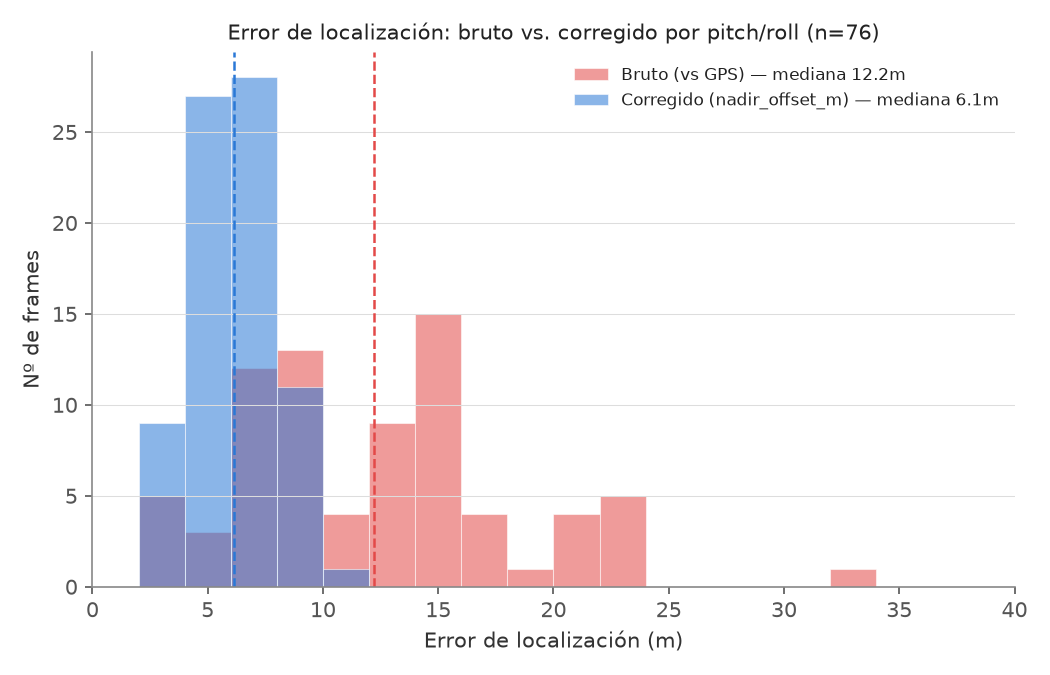
\includegraphics[width=0.8\textwidth]{error_localizacion.png}
\caption{Distribución del error de localización, bruto frente a corregido por actitud del dron (n=76).}
\label{fig:error-localizacion}
\end{figure}

\subsection{Efecto de la altitud de vuelo}
\label{sec:efecto-altitud}

El vuelo de validación cubre un rango de altitudes desde poco más de 60 m hasta 120 m, con dos tramos de vuelo relativamente estables alrededor de $\approx$80 m y $\approx$120 m (con una transición gradual entre ambos). Separando las 76 consultas por altitud (umbral en 100 m):

\begin{itemize}
\item \textbf{Consultas a $\approx$80 m} (\SI{41}{consultas}, altitud $<$ \SI{100}{\metre}): error mediana \SI{5.1}{\metre}, media \SI{5.1}{\metre}.
\item \textbf{Consultas a $\approx$120 m} (\SI{35}{consultas}, altitud $\geq$ \SI{100}{\metre}): error mediana \SI{7.2}{\metre}, media \SI{7.5}{\metre}.
\end{itemize}

El tramo a mayor altitud tiene un error algo mayor, coherente con que a más altura cada píxel del fotograma cubre más terreno real, por lo que un mismo error de proyección en píxeles se traduce en un error mayor en metros. Las Figuras \ref{fig:trayectoria-error-80m} y \ref{fig:trayectoria-error-120m} muestran, para cada tramo, la posición GNSS cruda, la posición corregida por actitud y la posición estimada por el pipeline, para cada consulta (sin conectarlas en una trayectoria continua entre fotogramas, ya que el \textit{pitch}/\textit{roll} real oscila de forma apreciable entre fotogramas consecutivos en este dron sin \textit{gimbal}, y conectar los puntos corregidos generaría un zigzag que no representa ningún desplazamiento real).

\begin{figure}[htbp]
\centering
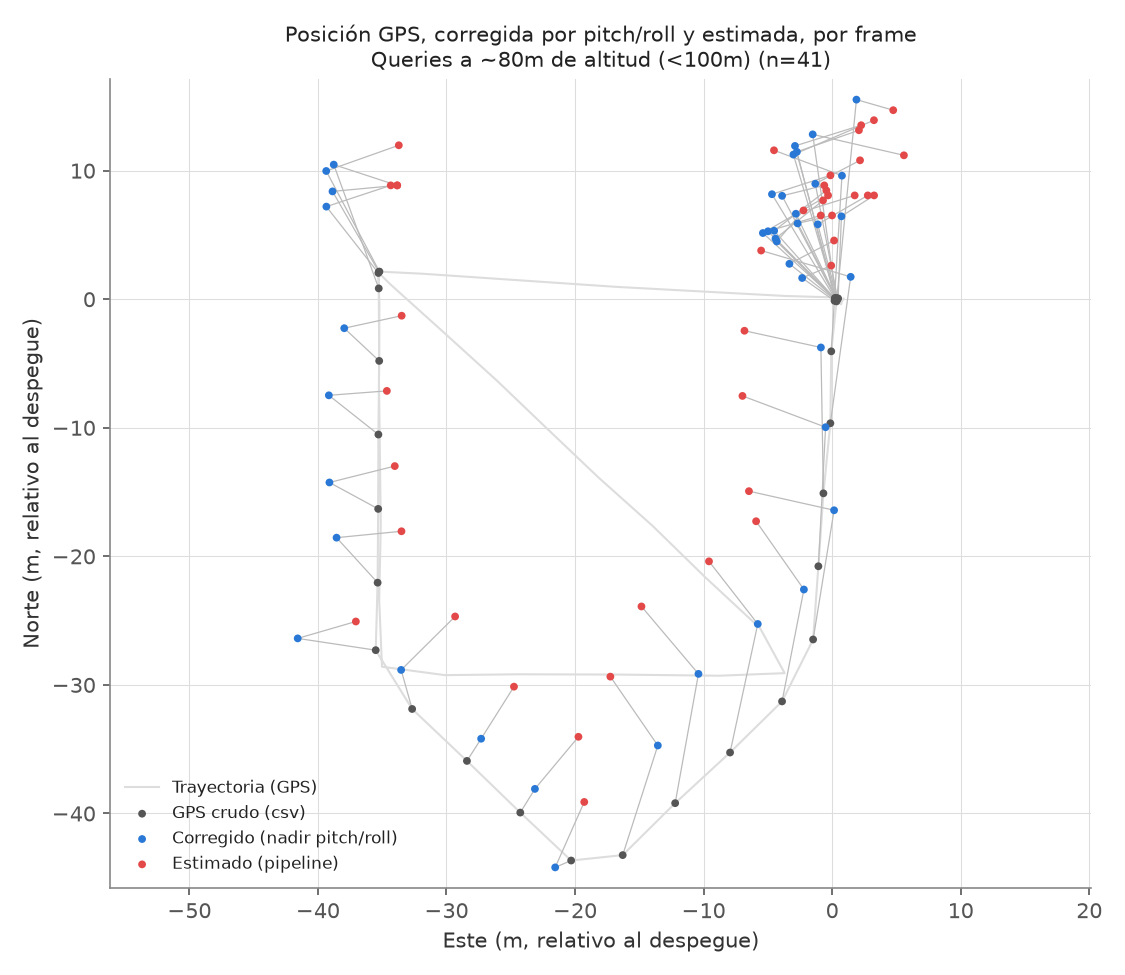
\includegraphics[width=0.8\textwidth]{trayectoria_error_80m.png}
\caption{Posición GNSS, corregida y estimada, para las consultas a $\approx$80 m de altitud (n=41).}
\label{fig:trayectoria-error-80m}
\end{figure}

\begin{figure}[htbp]
\centering
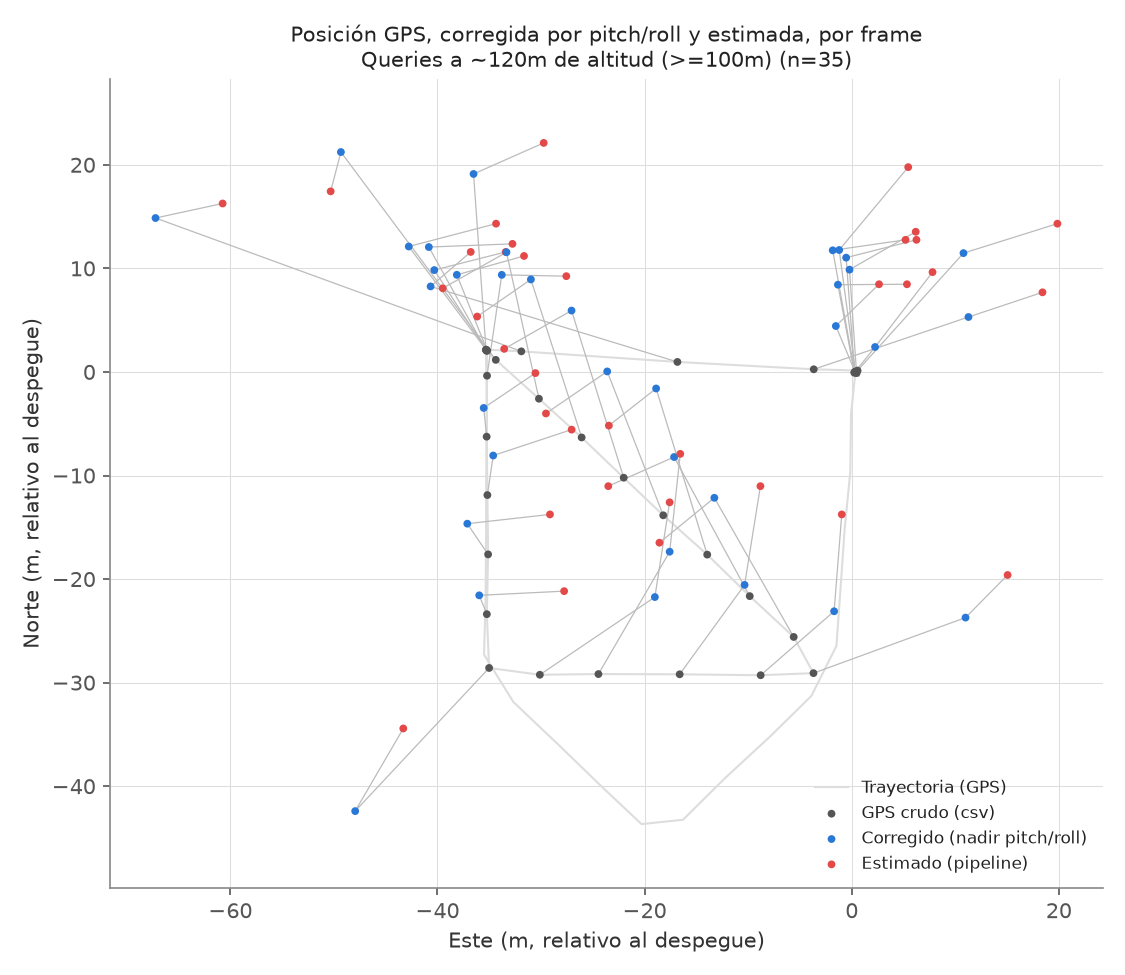
\includegraphics[width=0.8\textwidth]{trayectoria_error_120m.png}
\caption{Posición GNSS, corregida y estimada, para las consultas a $\approx$120 m de altitud (n=35).}
\label{fig:trayectoria-error-120m}
\end{figure}

\section{Análisis de rendimiento}
\label{sec:analisis-rendimiento}

El pipeline completo, ejecutado sobre un ordenador externo con GPU (NVIDIA GeForce RTX 3050 Laptop, 4 GB), tarda una media de \SI{0.41}{\second} por consulta (\SI{31.5}{\second} en total para las 76 consultas), de los cuales aproximadamente dos tercios corresponden a la extracción del descriptor VLAD+DINOv3-SAT y un tercio al emparejamiento LoFTR con \textit{early-exit} (\autoref{fig:tiempo-desglose} del \autoref{cap:geolocalizacion-visual}). Este tiempo no incluye la carga inicial de los modelos en memoria ($\approx$\SI{7}{\second} la primera consulta de cada sesión), que solo se paga una vez por proceso.

Esta cifra corresponde a la ejecución en un ordenador externo con GPU dedicada, no en la Raspberry Pi embarcada. La Raspberry Pi 3B+ utilizada en este proyecto no dispone de aceleración por GPU comparable ni de la memoria necesaria para cargar los modelos DINOv3-vitl16 y LoFTR simultáneamente; se ha usado únicamente para las tareas de captura, registro de telemetría y comunicaciones (\autoref{sec:limitaciones-software}), dejando la ejecución completa del pipeline visual fuera de bordo. No se ha intentado ejecutar el pipeline completo sobre la Raspberry Pi 3B+: dada su falta de aceleración GPU y de memoria suficiente para los modelos empleados, se considera inviable de antemano y no aporta información adicional medirlo directamente.

\subsection{Viabilidad de cómputo embarcado con aceleración GPU}
\label{sec:viabilidad-jetson}

Una Raspberry Pi no es la plataforma ideal para ejecutar el pipeline de geolocalización visual a bordo: se ha usado en este proyecto porque era el hardware disponible, no porque sea la opción de diseño recomendada. Para una futura ejecución embarcada en tiempo real, el candidato natural es una computadora con aceleración GPU de bajo consumo, como los módulos NVIDIA Jetson (p.\,ej. Jetson Orin Nano), pensados específicamente para inferencia de redes neuronales en el borde con un consumo de \SIrange{7}{25}{\watt}, frente a los \SIrange{115}{170}{\watt} de una GPU de portátil/sobremesa como la usada en este trabajo.

No se ha encontrado (ni realizado, al no disponer del hardware) un benchmark directo que compare exactamente el modelo usado en este proyecto (DINOv3-vitl16 + LoFTR) entre una RTX 3050 y una Jetson Orin Nano, por lo que aquí solo se ofrece una referencia de orden de magnitud a partir de benchmarks publicados de terceros sobre modelos comparables, no una estimación precisa para este pipeline concreto:

\begin{itemize}
\item Sobre Jetson Orin Nano, un \textit{Vision Transformer} ViT-B/16 (un backbone bastante más pequeño que el ViT-L/16 usado en este trabajo) tarda entre 17 y 20\,ms por imagen a resolución 224$\times$224 en FP16, y entre 41 y 49\,ms a 384$\times$384 \parencite{jetson_vit_benchmark}.
\item En otra comparativa publicada, para un modelo de lenguaje (BERT-Large, no visual, pero indicativo de la diferencia de arquitectura), una RTX 3060 de sobremesa resultó unas 7 veces más rápida que una Jetson AGX Xavier (un módulo Jetson de generación anterior y más potente que la Orin Nano) en inferencia FP16 \parencite{rtx_jetson_bert_benchmark}.
\end{itemize}

Con estas referencias, es razonable esperar que ejecutar este pipeline sobre una Jetson Orin Nano resultase en un tiempo por consulta varias veces mayor que en la RTX 3050 usada (los \SI{0.41}{\second}/consulta medidos), probablemente en el rango de 1--3 segundos por consulta, sin que esto deba tomarse como una estimación precisa, dado que ni el modelo (ViT-L/16, más grande que el ViT-B/16 de la referencia) ni la generación de Jetson coinciden exactamente con las referencias disponibles. Confirmar esta cifra con una medida real sobre hardware Jetson queda como trabajo futuro (\autoref{sec:trabajos-futuros}), y sería el paso necesario antes de decidir si esta familia de dispositivos permite una ejecución a bordo en tiempo real o si haría falta, además, seguir reduciendo el propio modelo (p.\,ej. una variante más pequeña de DINOv3, o cuantización a INT8).

\subsection{Efecto del radio y del zoom del mosaico de referencia}
\label{sec:efecto-radio-zoom}

Además del pipeline de matching, se evaluó el efecto de dos parámetros de la preparación del mosaico de referencia (\autoref{sec:generacion-mapa-base}) sobre precisión y tiempo, usando un subconjunto de 15 consultas muestreadas uniformemente de las 76 disponibles: el radio del área descargada (500, 1500, 3000 y 5000 m, a zoom fijo 18) y el nivel de zoom de las teselas (17, 18 y 19, a radio fijo 1500 m). La \autoref{fig:precision-radio-zoom} muestra el efecto sobre la precisión y la \autoref{fig:tiempo-query-radio-zoom} sobre el tiempo por consulta.

\begin{figure}[htbp]
\centering
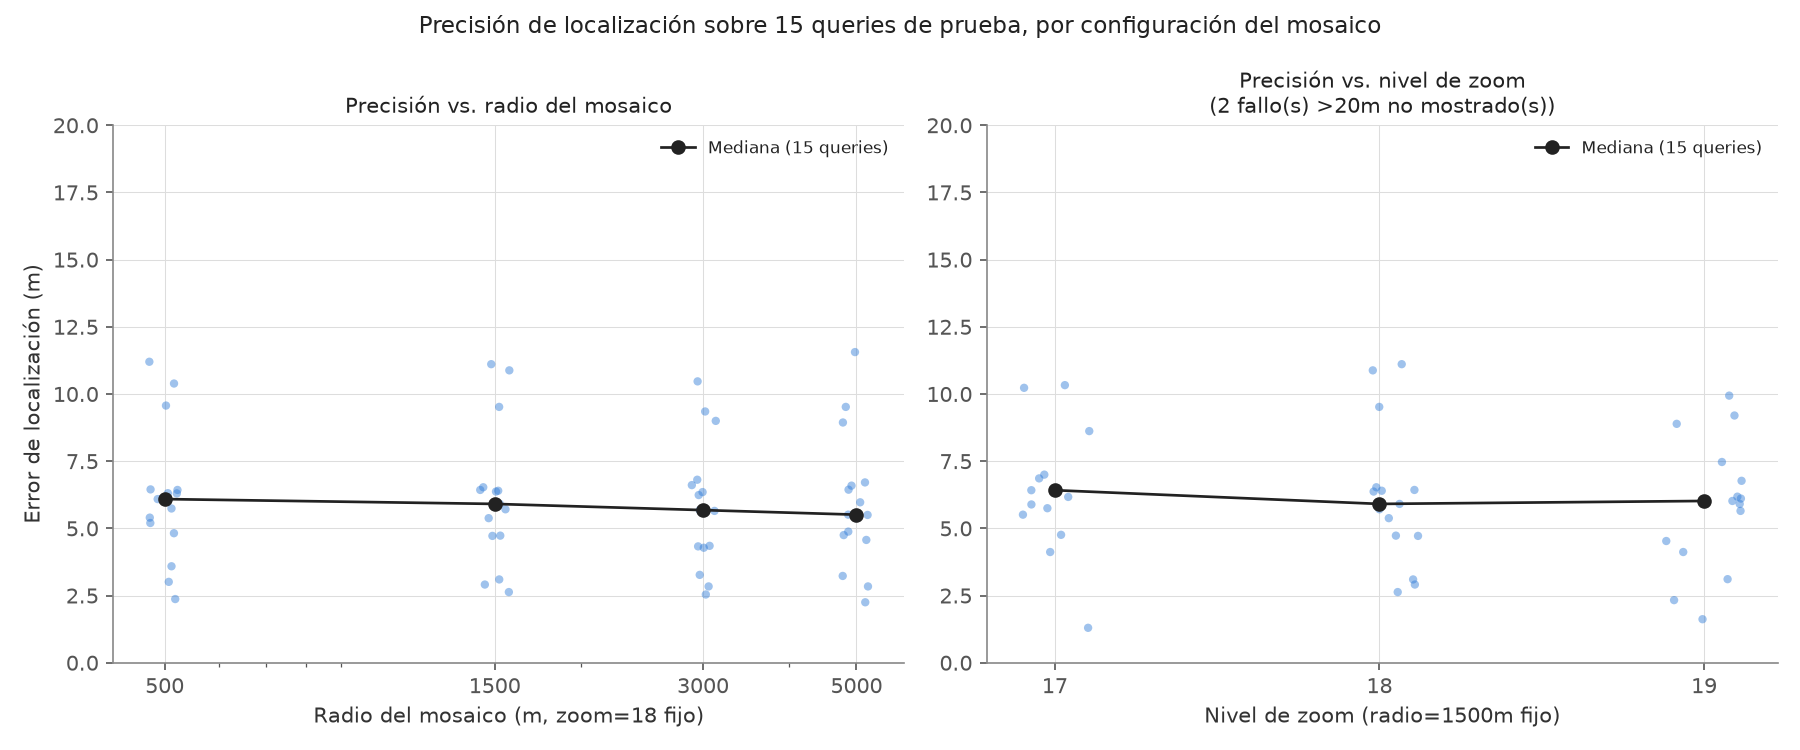
\includegraphics[width=\textwidth]{precision_radio_zoom.png}
\caption{Error de localización (15 consultas de prueba) según el radio del mosaico (zoom=18 fijo) y según el nivel de zoom (radio=1500\,m fijo).}
\label{fig:precision-radio-zoom}
\end{figure}

\begin{figure}[htbp]
\centering
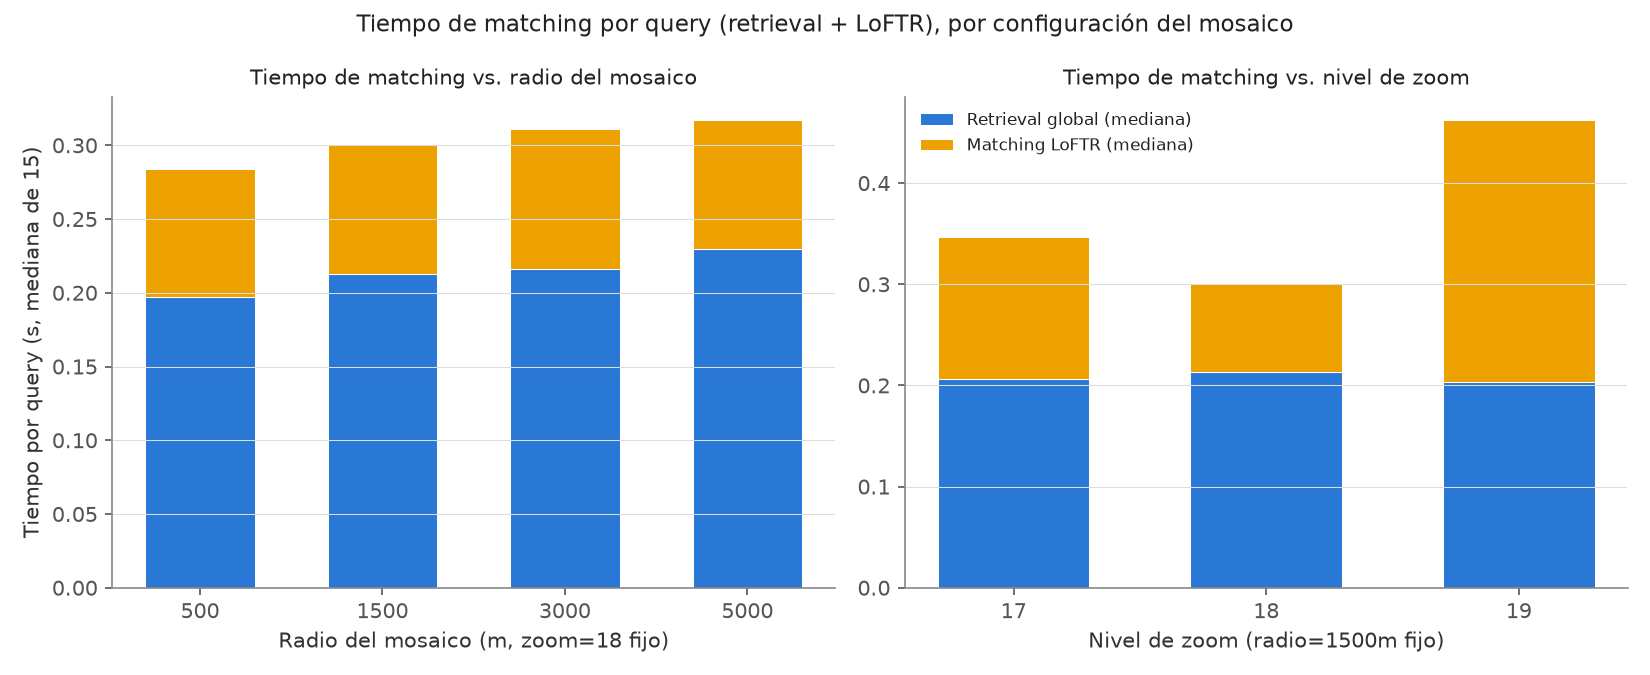
\includegraphics[width=\textwidth]{tiempo_query_radio_zoom.png}
\caption{Tiempo de matching por consulta (retrieval + LoFTR) según radio y zoom del mosaico.}
\label{fig:tiempo-query-radio-zoom}
\end{figure}

El radio del mosaico apenas afecta a la precisión (variación de \SI{0.6}{\metre} entre los extremos probados, dentro del ruido esperable con solo 15 consultas) pero sí al coste de preparación, que crece muy rápido con el área (\autoref{fig:tiempos-setup-radio-zoom}). El nivel de zoom 18 (el usado en producción) tiene la mejor mediana de error; el zoom 17 produjo 2 fallos catastróficos de $\approx$830 m sobre las mismas 15 consultas, y el zoom 19 no mejora la precisión pero sí el tiempo de descarga y de matching por consulta. Estos resultados confirman que la configuración de producción (radio 1500 m, zoom 18) es una elección razonable: aumentar el radio apenas mejora la precisión a mucho coste, y bajar el zoom introduce fallos raros pero severos.

\section{Discusión}
\label{sec:discusion-resultados}

Los resultados confirman que el sistema cumple los criterios de éxito definidos en el \autoref{sec:criterios-exito}: el dron capturó imágenes con marcas temporales y telemetría sincronizada en un vuelo real, y el pipeline de CVGL estimó la posición sobre las 76 consultas evaluadas con un error mediano de \SI{6.1}{\metre} sin ningún fallo total de emparejamiento.

Los principales factores que explican el error residual, de mayor a menor impacto observado, son: (1) la actitud instantánea del dron en el momento de captura, que sin corregir (\autoref{sec:correccion-nadir}) duplica el error medio; (2) la altitud de vuelo, con un error algo mayor a 120 m que a 80 m por la relación entre resolución en el suelo y altura; y (3) la resolución del mosaico de referencia (nivel de zoom), donde una resolución insuficiente no degrada la precisión típica pero sí introduce fallos catastróficos ocasionales. El radio del mosaico, en cambio, no resultó ser un factor relevante para la precisión en el rango evaluado.

% ---------------------------------------------------------------------


% ---------------------------------------------------------------------
% Planificación y presupuesto
% ---------------------------------------------------------------------

\chapter{Planificación y presupuesto}
\label{cap:planificacion-presupuesto}

\begin{Resumen}
Este capítulo describe la planificación temporal del proyecto por fases, los principales riesgos técnicos identificados y las medidas adoptadas para mitigarlos, y el presupuesto de los componentes empleados en la plataforma.
\end{Resumen}

\section{Planificación del proyecto}
\label{sec:planificacion-proyecto}

El proyecto puede dividirse en las siguientes fases de trabajo, distribuidas en el tiempo como recoge la \autoref{fig:gantt-proyecto}:

\begin{enumerate}
\item \textbf{Análisis inicial}: definición del alcance, selección de componentes y estudio de alternativas de navegación visual.
\item \textbf{Montaje hardware}: ensamblaje del chasis, motores, controlador, alimentación, GPS, cámara y Raspberry Pi.
\item \textbf{Configuración de vuelo}: calibración del controlador, pruebas de motores, parámetros de seguridad y validación en tierra.
\item \textbf{Integración software}: configuración de MAVProxy, Tailscale, \texttt{tmux}, captura de imágenes y registro de telemetría.
\item \textbf{Captura experimental}: vuelos de prueba, generación de datasets y revisión de la calidad de los datos.
\item \textbf{Evaluación CVGL}: creación de mapa base, galería satelital, recuperación global, matching local y análisis de error.
\item \textbf{Redacción}: documentación de diseño, resultados, conclusiones y líneas futuras.
\end{enumerate}

\begin{figure}[htbp]
\centering
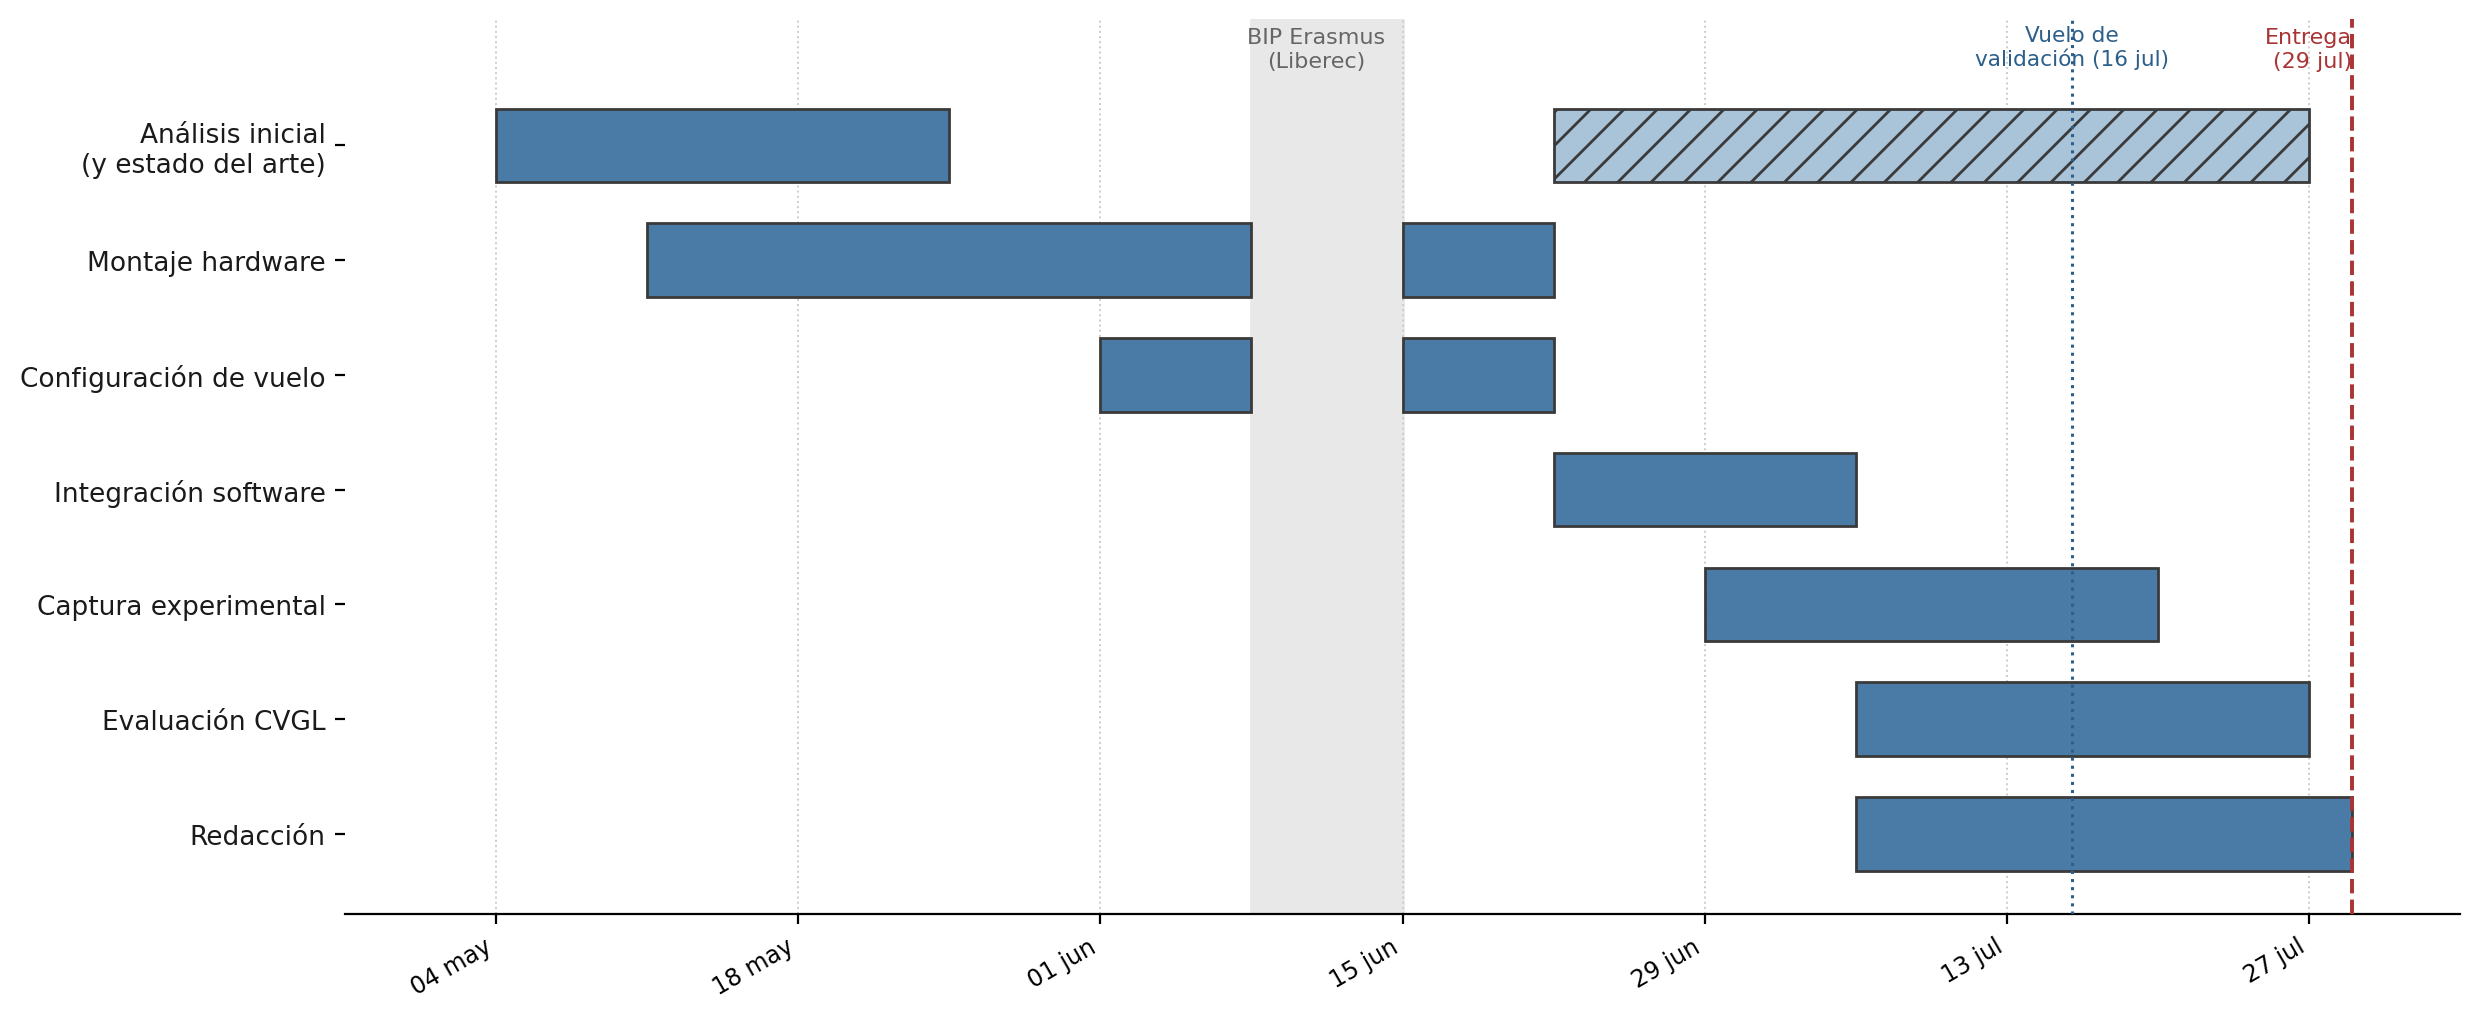
\includegraphics[width=\textwidth]{gantt_proyecto.png}
\caption{Planificación temporal del proyecto, desde la compra de componentes hasta la entrega de la memoria.}
\label{fig:gantt-proyecto}
\end{figure}

\section{Riesgos y medidas de mitigación}
\label{sec:riesgos-mitigacion}

La \autoref{tab:riesgos} resume los riesgos técnicos principales y las medidas previstas para reducir su impacto.

\begin{table}[htbp]
\centering
\caption{Riesgos técnicos del proyecto.}
\label{tab:riesgos}
\begin{tabularx}{\textwidth}{p{0.26\textwidth}X X}
\toprule
\textbf{Riesgo} & \textbf{Impacto} & \textbf{Mitigación} \\
\midrule
Vibraciones en cámara & Imágenes borrosas y peor matching visual. & Montaje antivibración, revisión de hélices y vuelos de prueba. \\
Pérdida de conexión remota & Interrupción de monitorización. & Uso de \texttt{tmux} y registro local en la Raspberry Pi. \\
Sobrecarga computacional & Imposibilidad de CVGL en tiempo real a bordo. & Evaluación fuera de bordo y propuesta de optimización futura. \\
Fallo de telemetría & Datos incompletos para evaluación. & Registro local, pruebas de MAVLink en tierra y comprobación previa al vuelo. \\
Autonomía insuficiente & Menor tiempo de captura. & Vuelos cortos e incrementales, control de carga y revisión de peso. \\
\bottomrule
\end{tabularx}
\end{table}

\section{Presupuesto}
\label{sec:presupuesto}

La \autoref{tab:presupuesto} recoge el presupuesto de los componentes de la plataforma. La Raspberry Pi, el dongle LTE, la emisora con su receptor FlySky FS-i6X y el material auxiliar ya se tenían de antes de empezar el proyecto (no se compraron para él), por lo que su coste se estima a precio aproximado de reposición en vez de a partir de un ticket de compra real.

\begin{longtable}{p{0.34\textwidth}p{0.12\textwidth}p{0.18\textwidth}p{0.18\textwidth}}
\caption{Presupuesto inicial del sistema.}\label{tab:presupuesto}\\
\toprule
\textbf{Elemento} & \textbf{Cantidad} & \textbf{Coste unitario} & \textbf{Subtotal} \\
\midrule
\endfirsthead
\toprule
\textbf{Elemento} & \textbf{Cantidad} & \textbf{Coste unitario} & \textbf{Subtotal} \\
\midrule
\endhead
Chasis F450 con tren de aterrizaje & 1 & 16.29€ & 16.29€ \\
Motores brushless 2212 920KV & 4 & 6.50€ & 26.00€ \\
Hélices 1045 CW/CCW & 1 lote de 10 & 6.67€ & 6.67€ \\
Batería LiPo 4S 5200 mAh 60C & 1 & 31.19€ & 31.19€ \\
Stack H743 6S con ESC 55 A & 1 & 51.69€ & 51.69€ \\
Módulo GPS M10 con brújula & 1 & 14.28€ & 14.28€ \\
BEC ajustable & 1 & 4.39€ & 4.39€ \\
Placa antivibración & 1 & 4.99€ & 4.99€ \\
Cámara USB global shutter & 1 & 65.99€ & 65.99€ \\
Raspberry Pi (ya disponible, coste aprox. de reposición) & 1 & 60.00€ & 60.00€ \\
Dongle LTE (ya disponible, coste aprox. de reposición) & 1 & 20.00€ & 20.00€ \\
Emisora y receptor FlySky FS-i6X (ya disponible, coste aprox. de reposición) & 1 & 45.00€ & 45.00€ \\
Material auxiliar, conectores y fijaciones (coste aprox.) & 1 lote & 10.00€ & 10.00€ \\
\midrule
\textbf{Total} & & & \textbf{356.49€} \\
\bottomrule
\end{longtable}

% ---------------------------------------------------------------------

% ---------------------------------------------------------------------
% Conclusiones
% ---------------------------------------------------------------------

\chapter{Conclusiones y trabajos futuros}
\label{cap:conclusiones}

\begin{Resumen}
Este capítulo recoge las conclusiones del trabajo a la luz de los resultados experimentales obtenidos sobre el vuelo de validación (\autoref{cap:experimentos-resultados}): un error de localización mediano de \SI{6.1}{\metre} sobre 76 consultas reales, sin ningún fallo de emparejamiento. Se resumen las aportaciones del trabajo y las líneas de mejora más relevantes identificadas durante el desarrollo.
\end{Resumen}

\section{Conclusiones}
\label{sec:conclusiones-provisionales}

El proyecto aborda la integración completa de una plataforma aérea personalizada para estudiar navegación basada en visión, y a diferencia de un enfoque puramente algorítmico sobre \textit{datasets} externos, obliga a resolver las restricciones reales de un sistema robótico embarcado: desde la reprogramación de la placa de vuelo tras perder su \textit{firmware} hasta la pérdida de señal GPS por proximidad a otros componentes (\autoref{sec:problemas-hardware}).

La arquitectura planteada separa correctamente las funciones críticas de vuelo de las tareas de percepción y registro. El controlador de vuelo se encarga de la estabilización y la misión, mientras que la Raspberry Pi captura imágenes, registra telemetría y mantiene comunicaciones mediante Tailscale y sesiones persistentes de \texttt{tmux}. Esta separación mejora la seguridad y facilita la depuración, y quedó validada en un vuelo real de más de 5 minutos con captura continua de 142 fotogramas y telemetría sincronizada, tras resolver un problema de desincronización mediante hilos independientes de captura y de telemetría (\autoref{sec:problema-sincronizacion-hilos}).

Sobre los datos de ese vuelo, el pipeline de CVGL final —recuperación global con VLAD sobre DINOv3 (variante SAT-493M), verificación local con LoFTR y MAGSAC++, y corrección del punto de referencia por la actitud del dron— logra una precisión de localización con error mediano de \SI{6.1}{\metre} sobre las 76 consultas evaluadas, sin ningún fallo total de emparejamiento. Esta cifra no es el resultado de adoptar directamente el primer enfoque razonable, sino de comparar empíricamente varias alternativas en cada etapa (backbone, agregación, calibración de cámara, tamaño y resolución del mosaico de referencia, optimizaciones de tiempo) y quedarse con la que realmente funciona mejor sobre esta escena y este hardware concretos, no con la que la literatura sugiere por defecto.

Una conclusión técnica importante es que la geolocalización visual completa requiere una capacidad de cálculo muy superior a la disponible en la Raspberry Pi 3B+ empleada (\autoref{sec:hardware-raspberry-comunicaciones}). La ejecución fuera de bordo no es una limitación del trabajo, sino una decisión de diseño deliberada: permite validar el algoritmo y cuantificar con precisión sus requisitos reales de cómputo y tiempo (\autoref{sec:analisis-rendimiento}) antes de plantear su optimización para ejecución embarcada en tiempo real.

\section{Aportaciones del trabajo}
\label{sec:aportaciones}

Las principales aportaciones del trabajo son:

\begin{enumerate}
\item diseño e integración de un dron propio orientado a captura de datos visuales georreferenciados, incluyendo la resolución de varios incidentes reales de integración hardware (\autoref{sec:problemas-hardware});
\item un flujo de captura robusto que asocia imagen y telemetría MAVLink de forma sincronizada mediante hilos independientes, con acceso remoto persistente mediante Tailscale y \texttt{tmux} tolerante a cortes de conexión;
\item un pipeline de CVGL completo (mapa base $\rightarrow$ galería $\rightarrow$ recuperación global $\rightarrow$ emparejamiento local $\rightarrow$ corrección geométrica $\rightarrow$ error) validado sobre un vuelo real, no solo sobre datos sintéticos o de terceros;
\item una comparación empírica sistemática de las alternativas de diseño del pipeline visual (2 agregaciones $\times$ 3 backbones para recuperación global; calibración de cámara; radio y zoom del mosaico de referencia; optimizaciones de LoFTR), documentando tanto lo que mejoró el resultado como lo que se probó y se descartó por no aportar mejora;
\item un análisis cuantitativo del efecto de la actitud del dron sobre el error de localización medido, y de una corrección geométrica que reduce el error medio a la mitad al comparar contra el punto de terreno real en vez de la posición cruda de la antena GNSS.
\end{enumerate}

\section{Trabajos futuros}
\label{sec:trabajos-futuros}

Como continuación natural del proyecto se proponen las siguientes líneas de trabajo:

\begin{itemize}
\item \textbf{Documentar y automatizar la calibración física de la cámara respecto al cuerpo del dron} (offset de montaje y orientación relativa al IMU), que sigue sin cuantificarse de forma independiente de la corrección de actitud ya aplicada (\autoref{sec:correccion-nadir}). No debe confundirse con la calibración de los parámetros \emph{intrínsecos} de la cámara (distorsión de lente), que sí se investigó explícitamente y se descartó por no aportar mejora de precisión, e incluso perjudicarla ligeramente por un artefacto de deformación en los bordes de la imagen corregida (\autoref{sec:estado-alternativas-no-adoptadas});
\item ampliar el conjunto de datos con vuelos en distintas zonas, condiciones de iluminación y estaciones del año, para evaluar la robustez del pipeline fuera de las condiciones del vuelo de validación;
\item seguir optimizando el pipeline visual para reducir su tiempo de inferencia: la configuración actual (VLAD+DINOv3-SAT con \textit{early-exit}, FP16 y tamaño de imagen reducido) ya reduce el tiempo medio por consulta a unos \SI{0.4}{\second} en un ordenador con GPU (frente a varios segundos sin optimizar), pero sigue siendo insuficiente para ejecución embarcada en tiempo real en la Raspberry Pi actual; una vía adicional, no explorada en este trabajo, es sustituir el descriptor VLAD+DINOv3-SAT —que sigue siendo \textit{zero-shot}, sin ningún ajuste sobre pares reales dron-satélite— por un descriptor afinado (\textit{fine-tuned}) específicamente sobre pares de imágenes dron-satélite de la propia zona de vuelo, lo que podría mejorar precisión y/o permitir un modelo más ligero para la misma tarea;
\item evaluar computadoras embarcadas con aceleración GPU (p.\,ej. Jetson) para ejecutar el pipeline de CVGL completo a bordo, sustituyendo a la Raspberry Pi 3B+ actual, que se ha usado deliberadamente solo para captura y comunicaciones (\autoref{sec:hardware-raspberry-comunicaciones});
\item integrar la posición estimada por visión como entrada auxiliar al sistema de navegación del dron (por ejemplo, inyectándola como una fuente de posición adicional en el filtro de estimación de ArduPilot), en vez de calcularse únicamente de forma \textit{offline} tras el vuelo;
\item estudiar la robustez del sistema ante pérdida real de GNSS durante el vuelo, cambios estacionales del terreno respecto al mosaico de referencia, y mapas de referencia de menor actualidad o resolución que los usados en este trabajo.
\end{itemize}

% ---------------------------------------------------------------------


% -------------------------------------------------------
% -------------------------------------------------------
% -------------------------------------------------------
% Bibliografía

\bibitemsep = 3ex
\bibhang = 2em

\printbibliography[heading=bibintoc,title=\bibname]


% -------------------------------------------------------
% Anexos

\appendix

% ---------------------------------------------------------------------
% Anexo de scripts
% ---------------------------------------------------------------------

\chapter{Scripts y archivos de apoyo}
\label{cap:anexo-scripts}

Este anexo recoge los scripts utilizados durante el proyecto, organizados en dos grupos: el \textbf{pipeline de producción} (carpeta \texttt{principal/}), que es la configuración final validada y la que se emplea para obtener los resultados del \autoref{cap:experimentos-resultados}, y los \textbf{scripts de experimentación} (carpeta \texttt{pruebas/}), usados para comparar alternativas (backbones, agregación, calibración de cámara, optimizaciones) antes de fijar la configuración final. Se documenta la función de cada archivo en vez de incluir el código completo, para no sobrecargar la memoria. El código fuente del pipeline de producción (\texttt{principal/}) está disponible públicamente en el repositorio del proyecto, \url{https://github.com/J7lio/TFG-Drone-Visual-Geolocalization}; los scripts de experimentación (\texttt{pruebas/}) no se publican por no tener el mismo nivel de cuidado ni ser necesarios para reproducir el resultado final, pero están disponibles bajo petición.

\subsection*{Pipeline de producción (\texttt{principal/})}

\begin{longtable}{p{0.36\textwidth}p{0.56\textwidth}}
\caption{Scripts del pipeline de producción.}\label{tab:scripts-principal}\\
\toprule
\textbf{Archivo} & \textbf{Función} \\
\midrule
\endfirsthead
\toprule
\textbf{Archivo} & \textbf{Función} \\
\midrule
\endhead
\texttt{capturar\_vuelo.py \newline (codigos\_dron)} & Captura imágenes desde la cámara USB en un hilo independiente, escucha telemetría MAVLink en otro hilo y guarda ambos sincronizados en un CSV por sesión (ver \autoref{sec:captura-imagenes-telemetria}). \\
\texttt{01\_download\_basemap.py} & Descarga un mosaico satelital georreferenciado (ESRI World Imagery) de la zona de vuelo y lo guarda como GeoTIFF. \\
\texttt{02\_tile\_basemap\_\newline gallery.py} & Divide el mosaico en parches solapados dimensionados según la huella de la cámara y crea el índice geográfico de la galería. \\
\texttt{10\_preparar\_queries\_\newline vuelo\_completo.py} & Normaliza los frames de vuelo: rotación a norte según \texttt{Rumbo\_Norte} y recorte central por altitud (ver \autoref{sec:planteamiento-cvgl}). \\
\texttt{11\_ejecutar\_vuelo\_\newline completo.py} & Ejecuta el pipeline completo (recuperación global + LoFTR/MAGSAC++ con early-exit y FP16) sobre todas las queries y calcula el error de localización. \\
\texttt{12\_graficos\_\newline resultados.py} & Genera las gráficas de resultados (trayectoria, error, desglose de tiempos) a partir del CSV de resultados. \\
\texttt{descriptor\_produccion.py} & Descriptor global de producción: carga del backbone DINOv3-vitl16 (variante SAT-493M), extracción de tokens de parche y agregación VLAD (ajuste de vocabulario k-means e interfaz única de descriptor). \\
\texttt{geo\_utils.py} & Utilidades de conversión píxel-coordenada, huella de cámara, escala Web Mercator, desplazamiento nadir por pitch/roll y distancia Haversine. \\
\bottomrule
\end{longtable}

\subsection*{Scripts de experimentación (\texttt{pruebas/})}

\begin{longtable}{p{0.36\textwidth}p{0.56\textwidth}}
\caption{Scripts de experimentación y comparación de alternativas.}\label{tab:scripts-pruebas}\\
\toprule
\textbf{Archivo} & \textbf{Función} \\
\midrule
\endfirsthead
\toprule
\textbf{Archivo} & \textbf{Función} \\
\midrule
\endhead
\texttt{03\_test\_global\_\newline retrieval.py} & Evalúa la recuperación global de parches sobre un conjunto reducido de queries de prueba. \\
\texttt{04\_local\_matching\_\newline loftr.py} & Ejecuta y ajusta el emparejamiento local con LoFTR sobre las queries de prueba. \\
\texttt{05\_visualize\_matches.py} & Genera imágenes de diagnóstico: correspondencias entre frame de dron y parche satelital, y comparación entre posición real y estimada sobre el mapa. \\
\texttt{06\_diagnose\_retrieval\_\newline rank.py} & Analiza en qué posición del ranking global aparece el parche geográficamente correcto. \\
\texttt{07\_benchmark\_\newline optimizaciones.py} & Compara early-exit, precisión FP16 y \texttt{MAX\_SIDE} reducido para optimizar el tiempo de LoFTR. \\
\texttt{08\_benchmark\_batching.py} & Evalúa el procesado por lotes de LoFTR (descartado: mejora modesta frente al riesgo de VRAM). \\
\texttt{09\_efficientloftr\_\newline test.py} & Compara EfficientLoFTR frente a LoFTR ajustado (descartado: no supera a la configuración de kornia ya optimizada). \\
\texttt{13\_comparar\_retrieval\_\newline metodos.py} & Compara la matriz completa de 2 agregaciones (GeM, VLAD) por 3 backbones (DINOv2, DINOv3-LVD, DINOv3-SAT) — resultado que fija la configuración de producción. \\
\texttt{14\_graficos\_comparacion\_\newline metodos.py} & Genera la gráfica comparativa de métodos de recuperación global. \\
\texttt{15\_test\_radio\_zoom\_\newline basemap.py} & Evalúa el efecto del radio y el nivel de zoom del mosaico de referencia en precisión y tiempo. \\
\texttt{16\_graficos\_radio\_\newline zoom.py} & Genera las gráficas del barrido de radio/zoom del mosaico. \\
\texttt{gallery\_cache.py} & Caché de descriptores GeM+DINOv2 (usado solo como referencia en la comparativa de métodos). \\
\bottomrule
\end{longtable}

% ---------------------------------------------------------------------

% ---------------------------------------------------------------------
% Anexo de checklist
% ---------------------------------------------------------------------

\chapter{Lista de comprobación para vuelos de prueba}
\label{cap:anexo-checklist}

Este anexo propone una lista de comprobación operativa para las pruebas de vuelo, junto con las consideraciones normativas que se han tenido en cuenta para la zona empleada en el vuelo de validación del \autoref{cap:experimentos-resultados}.

\section{Normativa aplicable y autorización de la zona de vuelo}
\label{sec:normativa-vuelo}

En España, la normativa de referencia para operaciones con aeronaves no tripuladas de uso civil es el marco europeo EASA (Reglamentos (UE) 2019/947 y 2019/945), complementado por la normativa nacional de AESA. Dicho marco divide la categoría Abierta en tres subcategorías (A1, A2 y A3) según la masa máxima al despegue de la aeronave, si dispone de marcado de clase CE, y las distancias de seguridad respecto a personas que se pueden garantizar durante el vuelo.

El dron de este proyecto es de construcción privada (no dispone de marcado de clase CE) y tiene una masa al despegue superior a \SI{250}{\gram} e inferior a \SI{25}{\kilo\gram}. Según la tabla de subcategorías del Reglamento (UE) 2019/947, esta combinación —construcción privada y masa en dicho rango— sitúa la operación en la \textbf{subcategoría A3}, que exige volar alejado de personas y de zonas urbanas o residenciales. Para el vuelo de validación del \autoref{cap:experimentos-resultados} se cumplieron los requisitos correspondientes a esta subcategoría: se respetó el límite de altura de \SI{120}{\metre} sobre el nivel del suelo, la zona de vuelo se comprobó libre de restricciones aéreas, y se mantuvo alejada de núcleos urbanos y de cualquier otra zona no permitida por la normativa general.

Con independencia de la subcategoría operacional, la normativa exige además que el operador esté dado de alta como operador UAS ante AESA, que el piloto remoto disponga del certificado de competencia correspondiente (curso y examen de la subcategoría A1/A3), y que la operación esté cubierta por un seguro de responsabilidad civil. Estos tres requisitos se cumplieron antes del vuelo de validación del \autoref{cap:experimentos-resultados}.

\section{Antes de conectar la batería}
\label{sec:checklist-antes-bateria}

\begin{itemize}
\item Revisar estructura, tornillos, brazos y tren de aterrizaje.
\item Comprobar que las hélices no presentan grietas o deformaciones.
\item Verificar que la cámara y la Raspberry Pi están correctamente fijadas.
\item Confirmar que la batería está cargada y en buen estado.
\item Revisar que no hay cables cerca de hélices o partes móviles.
\end{itemize}

\section{Antes de armar}
\label{sec:checklist-antes-armar}

\begin{itemize}
\item Comprobar recepción de GPS y brújula en la estación de tierra.
\item Verificar tensión de batería y ausencia de alarmas críticas.
\item Confirmar conexión Tailscale y acceso a la Raspberry Pi.
\item Iniciar sesión \texttt{tmux} y lanzar el proceso de captura.
\item Confirmar que se guardan imágenes y filas en \texttt{telemetria.csv}.
\item Revisar la misión cargada en QGroundControl.
\end{itemize}

\section{Después del vuelo}
\label{sec:checklist-despues-vuelo}

\begin{itemize}
\item Desarmar el dron y desconectar la batería.
\item Copiar la carpeta de vuelo al ordenador de procesado.
\item Revisar número de imágenes, tamaño de archivos y continuidad temporal.
\item Abrir el CSV para comprobar que la telemetría contiene valores coherentes.
\item Anotar incidencias de vuelo, condiciones de iluminación y observaciones.
\item Ejecutar una prueba rápida del pipeline CVGL sobre algunos frames representativos.
\end{itemize}

% ---------------------------------------------------------------------

% ---------------------------------------------------------------------
% Anexo de Objetivos de Desarrollo Sostenible (ODS)
% ---------------------------------------------------------------------

\chapter{Relación del trabajo con los Objetivos de Desarrollo Sostenible}
\label{cap:anexo-ods}

De acuerdo con el artículo 10.3 de la Normativa de Trabajos de Fin de Grado y Trabajos de Fin de Máster de la UPV (Consejo de Gobierno, 21/07/2022) y su Anexo I, este anexo recoge el grado de relación del TFG con los Objetivos de Desarrollo Sostenible (ODS) de la agenda 2030.

La \autoref{tab:ods} recoge únicamente los ODS con una relación real y directa con el trabajo; el resto se marca como \enquote{No procede} en vez de forzar una relación tangencial.

\begin{table}[htbp]
\centering
\caption{Grado de relación del trabajo con los Objetivos de Desarrollo Sostenible.}
\label{tab:ods}
\begin{tabularx}{\textwidth}{Xp{0.09\textwidth}p{0.09\textwidth}p{0.09\textwidth}p{0.16\textwidth}}
\toprule
\textbf{Objetivo de Desarrollo Sostenible} & \textbf{Alto} & \textbf{Medio} & \textbf{Bajo} & \textbf{No\newline procede} \\
\midrule
ODS 1. Fin de la pobreza. & & & & X \\
ODS 2. Hambre cero. & & & & X \\
ODS 3. Salud y bienestar. & & & & X \\
ODS 4. Educación de calidad. & & & & X \\
ODS 5. Igualdad de género. & & & & X \\
ODS 6. Agua limpia y saneamiento. & & & & X \\
ODS 7. Energía asequible y no contaminante. & & & & X \\
ODS 8. Trabajo decente y crecimiento económico. & & & & X \\
ODS 9. Industria, innovación e infraestructuras. & X & & & \\
ODS 10. Reducción de las desigualdades. & & & & X \\
ODS 11. Ciudades y comunidades sostenibles. & & X & & \\
ODS 12. Producción y consumo responsables. & & & & X \\
ODS 13. Acción por el clima. & & & & X \\
ODS 14. Vida submarina. & & & & X \\
ODS 15. Vida de ecosistemas terrestres. & & & & X \\
ODS 16. Paz, justicia e instituciones sólidas. & & & & X \\
ODS 17. Alianzas para lograr objetivos. & & & & X \\
\bottomrule
\end{tabularx}
\end{table}

\section*{Descripción de la alineación con los ODS de mayor relación}

\begin{itemize}
\item \textbf{ODS 9 (Alto)}: el trabajo desarrolla e integra una solución tecnológica de navegación autónoma basada en visión para un vehículo aéreo no tripulado, combinando un sistema empotrado embarcado (computadora de borde, controlador de vuelo, sensores) con un pipeline de visión por computador (descriptores visuales profundos, emparejamiento geométrico) diseñado y validado empíricamente sobre hardware real. Este tipo de integración hardware-software es directamente extrapolable a aplicaciones industriales de inspección, monitorización de infraestructuras o logística mediante drones.
\item \textbf{ODS 11 (Medio)}: la navegación por visión sin depender de la señal GNSS es especialmente relevante en entornos donde esta señal se degrada o no está disponible, como los entornos urbanos densos (por reflexión y bloqueo de la señal entre edificios, el llamado \enquote{cañón urbano}) o durante emergencias en las que la infraestructura de posicionamiento puede fallar. Aunque este trabajo no se centra en un caso de uso urbano concreto, la tecnología desarrollada y validada es aplicable a la resiliencia de los sistemas de navegación aérea en ciudades y comunidades.
\end{itemize}

% ---------------------------------------------------------------------



% -------------------------------------------------------
% Fin del documento

\end{document}

% ---------------------------------------------------------------------
% ---------------------------------------------------------------------
% ---------------------------------------------------------------------
